\setcounter{chapter}{3}
\chapter{有限温单粒子格林函数, 费曼图技术及其应用}
\begin{introduction}
\item 松原(Matsubara)格林函数
\item 物理量的表示
\item 松原格林函数的若干性质及傅里叶变换
\item 自由粒子的松原格林函数
\item 松原格林函数的 Lehmann 表示
\item 其他单粒子热力学格林函数(实时)
\item 相互作用绘景下的松原格林函数
\item Wick 定理
\item 松原格林函数的坐标空间费曼图规则
\item 松原格林函数的动量空间费曼图规则
\item 松原格林函数的频率求和方法
\item 松原格林函数的应用
\end{introduction}
目前为止我们讲到的三种格林函数都是零温情况的, 它们分别是因果格林函数, 推迟格林函数和超前格林函数. 其中, 因果格林函数可以利用 Wick 定理展开. 

现在要讨论的是有限温度下的系统. 可以引入有限温度下的因果、推迟和超前热力学格林函数, 但不能直接由零温格林函数通过代换基态平均得到. 此时必须考虑另外一种格林函数. 日本京都大学的松原教授提出一个非常巧妙的方案, 人们称为松原格林函数, 也称为虚时格林函数. 在有限温度中, 只有这种格林函数可以利用费曼图技术, 其他格林函数可以利用相互之间的关系式求出来. 下面介绍松原格林函数.
\section{松原(Matsubara)格林函数}
考虑有限温度时, 采用巨正则系综比较方便. 

巨正则系综下, 哈密顿量改写为: $\hat{H}\to \hat{H}-\mu\hat{N}\equiv \hat{K}$, 其中 $\mu$ 是系统的化学势, $\hat{N}$ 是总粒子数算符.

有限温情况下, 需要引入密度算符处理混合态: 
\begin{equation}
    \hat{\rho}\equiv \frac{\e^{-\beta\hat{K}}}{\Xi },
\end{equation}
其中 $\beta=1/k_{\fun{B}}T$, $\Xi$ 是巨正则系综的配分函数, 表达式为 
\begin{equation}
    \Xi=\fun{Tr}\lmi \e^{-\beta \hat{K}} \rmi.
\end{equation}
巨正则系综下, 有类似于正则系综中自由能的热力学势 
\begin{equation}
    \Omega\equiv -\frac{1}{\beta}\ln \Xi,
\end{equation}
配分函数可以用热力学势表示为 
\begin{equation}
    \Xi =\e^{-\beta\Omega},
\end{equation}
相应的可以把密度算符表示成 
\begin{equation}
    \hat{\rho}=\e^{\beta (\Omega-\hat{K})}.
\end{equation}
巨正则系综中, 算符的平均值可以用密度算符表示为 
\begin{equation}
    \lag \hat{A} \rag_T=\fun{Tr}\lmi \e^{\beta(\Omega-\hat{K})}\hat{A} \rmi,
\end{equation}
通常通过粒子数算符的平均值来确定化学势 $\mu$, 有 
\begin{equation}
    \lag \hat{N} \rag_T=\fun{Tr}\lmi \e^{\beta(\Omega-\hat{K}) }\hat{N} \rmi_\mu=N.
\end{equation}

设 $\hat{H}$ 不显含时间, 巨正则系综的场算符在诸绘景下可以表示为:
\begin{itemize}
    \item 薛定谔绘景: 
    \begin{equation}
        \hat{\psi}^{}_{\alpha}(\vct{x}),\quad \hat{\psi}_\beta^\dg (\vct{x}'). 
    \end{equation}
    \item 海森伯绘景: 
    \begin{equation}
        \hat{\psi}_{H\alpha}^{ }(\vct{x},\tau)\equiv \e^{\hat{K}\tau}\hat{\psi}_\alpha(\vct{x})\e^{-\hat{K}\tau},\quad \hat{\psi}^\dg_{H\alpha}(\vct{x},\tau)\equiv \e^{\hat{K}\tau}\hat{\psi}_\alpha^\dg (\vct{x})\e^{-\hat{K}\tau}.
    \end{equation}
    与零温情况相比, $\tau\to \ii t$ 称为虚时, 取值范围 $\tau \in [0,\beta]$. 此处需要注意的是, 虚时情况的海森伯绘景场算符并不是厄米算符, 即 
    \begin{equation}
        \hat{\psi}_{H\alpha} (\vct{x},\tau)\ne \lmi \hat{\psi}^{}_{H\alpha}(\vct{x},\tau) \rmi^\dg.
    \end{equation}
\end{itemize}
有限温格林函数将采用海森伯绘景下的虚时场算符. 下面给出松原格林函数的定义.

\begin{definition}{松原格林函数}{}
  \begin{align}
        \mathcal{G}_{\alpha\beta}(\vct{x},\tau; \vct{x}',\tau')\equiv& -\fun{Tr}\lmi \hat{\rho}\hat{T}^{}_\tau \left[\hat{\psi}^{ }_{H\alpha}(\vct{x},\tau)\hat{\psi}^\dg_{H\beta}(\vct{x}',\tau')\right] \rmi\nonumber\\
        =&-\llag \hat{T}^{}_\tau \lmi \hat{\psi}_{H\alpha}^{ }(\vct{x},\tau)\hat{\psi}_{H\beta}^\dg (\vct{x}',\tau') \rmi \rrag_T.
    \end{align}
\end{definition}
\section{物理量的表示}
\subsection{单体算符的平均值}
单体算符的一般表达式为 
\begin{equation}
    F_2^{(1)}=\sum_\alpha\sum_\beta\int\hat{\psi}_\alpha^\dg (\vct{x})\hat{f}_{\alpha\beta}(\vct{x})\hat{\psi}_\beta^{ }(\vct{x})\dd \vct{x},
\end{equation}
单体算符在有限温下的平均值表示为 
    \begin{align}
        \llag \hat{F}_2^{(1)} \rrag_T=&\sum_\alpha\sum_\beta\int\dd \vct{x}\fun{Tr}\lmi \hat{\rho}\hat{\psi}_\alpha^\dg (\vct{x})\hat{f}_{\alpha\beta}(\vct{x})\hat{\psi}_\beta^{ }(\vct{x}) \rmi\nonumber\\
        =&\sum_\alpha\sum_\beta\int\dd \vct{x}\lim_{\vct{x}'\to \vct{x}}\hat{f}^{}_{\alpha\beta}(\vct{x})\fun{Tr}\lmi \hat{\rho}\hat{\psi}_\alpha^\dg(\vct{x}')\hat{\psi}_\beta^{ }(\vct{x}) \rmi\nonumber\\
        =&\sum_\alpha\sum_\beta\int\dd \vct{x}\lim_{\vct{x}'\to \vct{x}}\hat{f}^{}_{\alpha\beta}(\vct{x})\fun{Tr}\lmi \hat{\rho}\e^{-\hat{K}\tau}\hat{\psi}_{H\alpha}^\dg (\vct{x}',\tau)\e^{\hat{K}\tau} \e^{-\hat{K}\tau}\hat{\psi}_{H\beta}^{ }(\vct{x},\tau)\e^{\hat{K}\tau} \rmi\nonumber\\
        =&\sum_\alpha\sum_\beta\int\dd \vct{x}\lim_{\vct{x}'\to \vct{x}\atop \tau'\to \tau^+}\hat{f}^{}_{\alpha\beta}(\vct{x})\fun{Tr}\lmi \hat{\rho}\hat{\psi}_{H\alpha}^\dg (\vct{x}',\tau')\hat{\psi}_{H\beta}^{ }(\vct{x},\tau) \rmi\nonumber\\
        =&\sum_\alpha\sum_\beta\int\dd \vct{x}\lim_{\vct{x}'\to \vct{x}\atop \tau'\to \tau^+}\hat{f}^{}_{\alpha\beta}(\vct{x})\fun{Tr}\lmi \hat{\rho}\hat{T}_{\tau}\left[\hat{\psi}_{H\alpha}^\dg (\vct{x}',\tau')\hat{\psi}_{H\beta}^{ }(\vct{x},\tau)\right] \rmi\nonumber\\
        =&\pm\sum_\alpha\sum_\beta\int\dd \vct{x}\lim_{\vct{x}'\to \vct{x}\atop \tau'\to \tau^+}\hat{f}^{}_{\alpha\beta}(\vct{x})\fun{Tr}\lmi \hat{\rho}\hat{T}_{\tau}\left[\hat{\psi}_{H\beta}^{ }(\vct{x},\tau)\hat{\psi}_{H\alpha}^\dg (\vct{x}',\tau')\right] \rmi\nonumber\\
        =&\mp\sum_\alpha\sum_\beta\int\dd \vct{x}\lim_{\vct{x}'\to \vct{x}\atop \tau'\to \tau^+}\hat{f}^{}_{\alpha\beta}(\vct{x}) \mathcal{G}_{\beta\alpha}(\vct{x},\tau; \vct{x}',\tau').
    \end{align}
若 $\hat{f}_{\alpha\beta}$ 与自旋无关, 即
\begin{equation}
\hat{f}_{\alpha\beta}=\hat{f}\delta_{\alpha\beta},
\end{equation}
则有
\begin{equation}
 \llag \hat{F}_2^{(1)} \rrag_T=\mp\sum_\alpha\int\dd \vct{x}\lim_{\vct{x}'\to \vct{x}\atop \tau'\to \tau^+}\hat{f}(\vct{x}) \mathcal{G}_{\alpha\alpha}(\vct{x},\tau; \vct{x}',\tau').
\end{equation}

\begin{example}总动量算符

\begin{equation}
\langle\hat{T}\rangle_T=\mp\sum_\alpha\int\dd \vct{x}\lim_{\vct{x}'\to \vct{x}\atop \tau'\to \tau^+}\left(-\frac{\nabla_x^2}{2m}\right) \mathcal{G}_{\alpha\alpha}(\vct{x},\tau; \vct{x}',\tau').
\end{equation}
\end{example}

\begin{example}总粒子数算符

\begin{equation}
\langle\hat{N}\rangle_T=\mp\sum_\alpha\int\dd \vct{x}\lim_{\vct{x}'\to \vct{x}\atop \tau'\to \tau^+} \mathcal{G}_{\alpha\alpha}(\vct{x},\tau; \vct{x}',\tau').
\end{equation}
\end{example}

\begin{example}总自旋算符

\begin{equation}
\langle \hat{S} \rangle_T=\mp\sum_\alpha\sum_\beta\int\dd \vct{x}\lim_{\tau'\to \tau^+}S_{\alpha\beta}\mathcal{G}_{\beta\alpha}(\vct{x},\tau; \vct{x},\tau').
\end{equation}
\end{example}

\subsection{两体相互作用}
两体相互作用可以写作
\begin{equation}
\hat{V}=\frac{1}{2}\sum_{\alpha}\sum_\beta\iint\mathrm{d}\vct x \mathrm{d} \vct x' \hat{\psi}_{\alpha}^{\dg}(\vct x) \hat{\psi}_{\beta}^{\dg}(\vct x')\hat{V}(\vct x-\vct x')\hat{\psi}_{\beta}^{}(\vct x')\hat{\psi}_{\alpha}^{}(\vct x),
\end{equation}
考虑两体相互作用与自旋无关, 则两体相互作用的平均值为
\begin{equation}
\langle\hat{V}\rangle_T=\mp \frac{1}{2} \sum_\alpha \int \mathrm{d} \vct{x} \lim _{\substack{\vct{x}^{\prime} \rightarrow \vct{x} \\ \tau^{\prime} \rightarrow \tau^{+}}}\left[-\frac{\partial}{\partial \tau}+\frac{\nabla_{\vct x}^2}{2 m}+\mu\right] \mathcal{G}_{\alpha \alpha}\left(\vct{x}, \tau ; \vct{x}^{\prime}, \tau^{\prime}\right) .
\end{equation}

\subsection{内能}
内能可以表示为体系哈密顿量的热力学平均, 即
\begin{align}
E=&\langle\hat{H}\rangle_T=\langle\hat{T}\rangle_T+\langle\hat{V}\rangle_T\nonumber\\
=&\mp \frac{1}{2} \sum_\alpha \int \mathrm{d} \vct{x} \lim _{\substack{\vct{x}^{\prime} \rightarrow \vct{x}\\ \tau^{\prime} \rightarrow \tau^{+}}}\left[-\frac{\partial}{\partial \tau}-\frac{\nabla_{\vct x}^2}{2 m}+\mu\right] \mathcal{G}_{\alpha \alpha}\left(\vct{x}, \tau ; \vct{x}^{\prime}, \tau^{\prime}\right) .
\end{align}

\subsection{热力学势 $\Omega$ 的计算公式}
巨正则系综下, 热力学势 $\Omega$ 是一个很重要的物理量. 如果可以计算出体系的热力学势, 就可以得到体系的很多信息. 仿照上一章计算零温基态能的第二种方式, 引入如下赝哈密顿量:
\begin{equation}
\hat{H}(\lambda)=\hat{H}_0+\lambda \hat{H}_1,
\end{equation}
其中 $\lambda \in[0,1]$. $\hat{H}_0$ 表示自由粒子体系的哈密顿量, 通常是总动能 $\hat{T}$. $\hat{H}_1$ 表示粒子间的相互作用, 通常考虑两体相互作用 $\hat{V}$. $\lambda=0$ 时, $\hat{H}(0)$ 表示不考虑相互作用的自由粒子体系的哈密顿量; $\lambda=1$ 时, $\hat{H}(1)$ 是相互作用体系真实的哈密顿量; $(0,1)$ 区间内的 $\lambda$ 对应的哈密顿量 $\hat{H}(\lambda)$, 只是为了方便数学计算, 并不对应实际的哈密顿量. 对于巨正则系综, 还可以引入:
\begin{equation}
\hat{K}(\lambda)=\hat{H}(\lambda)-\mu \hat{N}=\hat{H}_0-\mu \hat{N}+\lambda \hat{H}_1\equiv\hat{K}_0+\lambda \hat{K}_1,
\end{equation}
其中
\begin{equation}
\hat{K}_0 \equiv \hat{H}_0-\mu \hat{N}, \quad \hat{K}_1 \equiv \hat{H}_1.
\end{equation}
按巨配分函数的定义, 可以得到 $\hat{K}(\lambda)$ 对应的巨配分函数:
\begin{equation}
\Xi(\lambda)=\operatorname{Tr}\left[\e^{-\beta \hat{K}(\lambda)}\right],
\end{equation}
则赝哈密顿量 $\hat{H}(\lambda)$ 对应的热力学势为:
\begin{equation}
\Omega(\lambda)=-\frac{1}{\beta} \ln \Xi(\lambda) .
\end{equation}
如果我们计算出松原格林函数表示巨配分函数 $\Xi(\lambda)$ 的形式, 很快就可以得到用松原格林函数表示热力学势 $\Omega(\lambda)$ 的表达式, 但是 $\Xi(\lambda)$ 的松原格林函数表示形式并不容易得到. 按之前计算基态能的方法, 在上式两边对 $\lambda$ 求偏导, 得到:
\begin{equation}
\frac{\partial \Omega(\lambda)}{\partial \lambda}=-\frac{1}{\beta} \frac{1}{\Xi(\lambda)} \frac{\partial \Xi(\lambda)}{\partial \lambda},
\end{equation}
这样上式两边再对 $\lambda$ 从 0 到 1 积分就可以得到相互作用体系的热力学势 $\Omega=\Omega(1)$ 的表达式, 这似乎还是需要计算 $\Xi(\lambda)$, 而且还要计算 $\displaystyle\frac{\partial \Xi(\lambda)}{\partial \lambda}$ . 但在实际计算过程中, $\Xi(\lambda)$ 会被消去, 只需要计算 $\displaystyle\frac{\partial \Xi(\lambda)}{\partial \lambda}$. 下面就来计算这一项:
\begin{align}
\frac{\partial \Xi(\lambda)}{\partial \lambda} =&\frac{\partial}{\partial \lambda} \operatorname{Tr}\left[\sum_{n=0}^{\infty} \frac{[-\beta \hat{K}(\lambda)]^n}{n !}\right]\nonumber \\
=&\sum_{n=0}^{\infty} \frac{(-\beta)^n}{n !} \operatorname{Tr}\left[\frac{\partial}{\partial \lambda}\left(\hat{K}_0+\lambda \hat{K}_1\right)^n\right] \nonumber\\
=&\sum_{n=1}^{\infty} \frac{(-\beta)^n}{n !} \operatorname{Tr}\left[n\left(\hat{K}_0+\lambda \hat{K}_1\right)^{(n-1)}\hat{K}_1\right]\nonumber\\
=&(-\beta) \sum_{n=1}^{\infty} \frac{(-\beta)^{(n-1)}}{(n-1) !} \operatorname{Tr}\left[\left(\hat{K}_0+\lambda \hat{K}_1\right)^{(n-1)} \hat{K}_1\right]\nonumber \\
\stackrel{m=n-1}{\longrightarrow} &(-\beta) \sum_{m=0}^{\infty} \frac{(-\beta)^m}{m !} \operatorname{Tr}\left[\left(\hat{K}_0+\lambda \hat{K}_1\right)^m \hat{K}_1\right]\nonumber \\
=&(-\beta) \operatorname{Tr}\left[\e^{-\beta \hat{K}(\lambda)} \hat{K}_1\right] \nonumber\\
=&-\frac{\beta}{\lambda} \e^{-\beta \Omega(\lambda)} \operatorname{Tr}\left[\e^{\beta(\Omega(\lambda)-\hat{K}(\lambda))} \lambda \hat{K}_1\right] \nonumber\\
=&-\frac{\beta}{\lambda} \e^{-\beta \Omega(\lambda)}\left\langle\lambda \hat{K}_1\right\rangle_\lambda,
\end{align}
这里利用了密度矩阵的表达式，最后的均值与 $\lambda$ 有关，而且是将 $\lambda \hat{K}_1$ 看成一个整体的相互作用进行计算, 所以 $\lambda$ 不能提出来消去. 故:
\begin{equation}
\frac{\partial \Omega(\lambda)}{\partial \lambda}=-\frac{1}{\beta}\frac{1}{\Xi(\lambda)}\left[-\frac{\beta}{\lambda} \e^{-\beta \Omega(\lambda)}\left\langle\lambda \hat{K}_1\right\rangle_\lambda\right]=\frac{\left\langle\lambda \hat{K}_1\right\rangle_\lambda}{\lambda},
\end{equation}
其中利用了热力学势与巨配分函数的关系式. 这样两边对 $\lambda$ 积分得到:
\begin{equation}
\left.\Omega(\lambda)\right|_0 ^1=\int_0^1 \mathrm{~d} \lambda \frac{\left\langle\lambda \hat{K}_1\right\rangle_\lambda}{\lambda}
\end{equation}
最终得到:
\begin{equation}
\Omega=\Omega_0+\int_0^1 \mathrm{~d} \lambda \frac{\left\langle\lambda \hat{K}_1\right\rangle_\lambda}{\lambda},
\end{equation}
其中 $\Omega_0$ 是自由粒子体系的热力学势. 考虑两体相互作用, 即 $\hat{K}_1=\hat{H}_1=\hat{V}$, 参考利用松原格林函数表示 $\hat{V}$ 的表达式, 可以得到完全类似的 $\lambda \hat{K}_1$ 的表达式 (将整个 $\lambda \hat{K}_1$ 看成 $\hat{V}$, 此时的松原格林函数将与 $\lambda$ 有关). 这样可以得到用松原格林函数表示热力学势的最终表达式:
\begin{equation}
\Omega=\Omega_0 \mp \frac{1}{2}\sum_\alpha\int_0^1 \frac{\mathrm{d} \lambda}{\lambda}   \int \mathrm{d} \vct{x} \lim _{\substack{\vct{x}^{\prime} \rightarrow \vct{x} \\ \tau^{\prime} \rightarrow \tau^{+}}}\left[-\frac{\partial}{\partial \tau}+\frac{\nabla_{\vct x}^2}{2 m}+\mu\right] \mathcal{G}\left(\vct{x}, \tau ; \vct{x}^{\prime}, \tau^{\prime} ; \lambda\right) .
\end{equation}

有了热力学势, 就可以得到诸多物理量:
\begin{align}
\langle \hat N \rangle_T &= -\left(\frac{\partial \Omega}{\partial \mu}\right)_{T,V};\\
P &= -\left(\frac{\partial \Omega}{\partial V}\right)_{\mu ,T};\\
S &= -\left(\frac{\partial \Omega}{\partial T}\right)_{\mu ,V}.
\end{align}

\section{松原格林函数的若干性质及傅里叶变换}
\subsection{松原格林函数的对称性}
与零温单粒子格林函数相同, 当体系(或哈密顿量)具有某种对称性, 相应的松原格林函数可以进行简化:
\begin{itemize}
\item 若 $\hat{H}$ 不显含时间, 则 
\begin{equation}
\mathcal{G}_{\alpha \beta}\left(\vct{x}, \tau ; \vct{x}^{\prime}, \tau^{\prime}\right)=\mathcal{G}_{\alpha \beta}\left(\vct{x}, \vct{x}^{\prime} ; \tau-\tau^{\prime}\right);
\end{equation}\\
\item 若体系是空间均匀的, 即 $[\hat{H}, \hat{\vct{P}}]_{-}=0$, 其中$\hat{\vct{P}}$是总动量算符, 则
\begin{equation}
\mathcal{G}_{\alpha \beta}\left(\vct{x}, \tau ; \vct{x}^{\prime}, \tau^{\prime}\right)=\mathcal{G}_{\alpha \beta}\left(\vct{x}-\vct{x}^{\prime} ; \tau, \tau^{\prime}\right);
\end{equation}\\
\item 若相互作用与自旋无关, 则 
\begin{equation}
\mathcal{G}_{\alpha \beta}\left(\vct{x}, \tau ; \vct{x}^{\prime}, \tau^{\prime}\right)=\delta_{\alpha \beta} \mathcal{G}\left(\vct{x}, \tau ; \vct{x}^{\prime}, \tau^{\prime}\right),
\end{equation}
其中 
\begin{equation}
\mathcal{G}\left(\vct{x}, \tau ; \vct{x}^{\prime}, \tau^{\prime}\right)=\frac{\sum\limits_{ \alpha} \mathcal{G}_{\alpha \alpha}\left(\vct{x}, \tau ; \vct{x}^{\prime}, \tau^{\prime}\right)}{2 S+1}.
\end{equation} 
\end{itemize}
\subsection{松原格林函数的周期性与反周期性}
考虑体系的哈密顿量不显含时间, 即 
\begin{equation}
\mathcal{G}_{\alpha \beta}\left(\vct{x}, \tau ; \vct{x}^{\prime}, \tau^{\prime}\right)=\mathcal{G}_{\alpha \beta}\left(\vct{x}, \vct{x}^{\prime} ; \tau-\tau^{\prime}\right)\equiv\mathcal{G}_{\alpha \beta}\left(\vct{x}, \vct{x}^{\prime} ; \tilde{\tau}\right).
\end{equation} 
这里定义了 $ \tilde{\tau}\equiv\tau-\tau^{\prime}$, 由 $\tau, \tau^{\prime} \in[0, \beta]$ 可知 $\tilde{\tau} \in[-\beta, \beta]$. 这时可以得出松原格林函数有如下周期性(反周期性):
\begin{equation}
\mathcal{G}_{\alpha \beta}\left(\vct{x}, \vct{x}^{\prime} ; \tilde{\tau}<0\right)=\pm \mathcal{G}_{\alpha \beta}\left(\vct{x}, \vct{x}^{\prime} ; \tilde{\tau}+\beta>0\right),
\end{equation}
其中 $+$ 对应玻色子, $-$ 对应费米子. 将该关系表示在数轴上, 如图\ref{period}所示.
\begin{figure}[htbp]
    \centering
    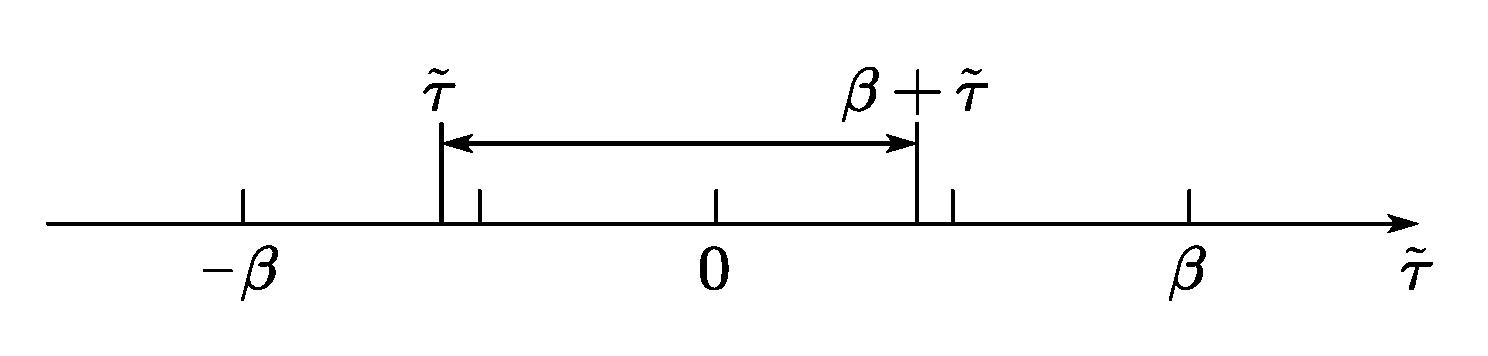
\includegraphics[width=8.5cm]{figure/period.pdf}
    \caption{松原格林函数的周期性(反周期性).}
    \label{period}
\end{figure}
\\下面来证明这一关系.
\begin{proof}
由松原格林函数的定义式:
\begin{equation}
\mathcal{G}_{\alpha \beta}\left(\vct{x}, \vct{x}^{\prime} ; \tilde{\tau}\right)=-\operatorname{Tr}\left[\e^{\beta(\Omega-\hat{K})} \hat{T}_\tau\left[\hat{\psi}^{}_{H \alpha}(\vct{x}, \tilde{\tau}) \hat{\psi}_{H\beta}^{\dagger}\left(\vct{x}^{\prime}\right)\right]\right],
\end{equation}
可以看出由于虚时编时乘积的作用, $\tilde{\tau}>0$ 和 $\tilde{\tau}<0$ 时的松原格林函数的表达式不同, 由此引入了周期性或反周期性. 下面分别讨论这两种情况下松原格林函数的表达式.

(i) $\tau>\tau^{\prime}$, 即 $\tilde{\tau}>0$:
\begin{equation}
\mathcal{G}^{(1)}_{\alpha \beta}\left(\vct{x}, \vct{x}^{\prime} ; \tilde{\tau}\right)  =-\operatorname{Tr}\left[\e^{\beta(\Omega-\hat{K})} \hat{\psi}^{}_{H \alpha}(\vct{x}, \tilde{\tau}) \hat{\psi}_{H\beta}^{\dagger}\left(\vct{x}^{\prime}\right)\right] ;
\end{equation}

(ii) $\tau<\tau^{\prime}$, 即 $\tilde{\tau}<0$:
\begin{align}
\mathcal{G}^{(2)}_{\alpha \beta}\left(\vct{x}, \vct{x}^{\prime} ; \tilde{\tau}\right) & =\mp \operatorname{Tr}\left[\e^{\beta(\Omega-\hat{K})} \hat{\psi}_{H\beta}^{\dagger}\left(\vct{x}^{\prime}\right) \hat{\psi}^{}_{H \alpha}(\vct{x}, \tilde{\tau})\right] \nonumber\\
& =\mp \operatorname{Tr}\left[\e^{\beta(\Omega-\hat{K})} \hat{\psi}_{H\beta}^{\dagger}\left(\vct{x}^{\prime}\right) \e^{\hat{K} \tilde{\tau}} \hat{\psi}^{}_\alpha(\vct{x}) \e^{-\hat{K} \tilde{\tau}}\right]\nonumber \\
& =\mp \operatorname{Tr}\left[\e^{\hat{K} \tilde{\tau}} \hat{\psi}^{}_\alpha(\vct{x}) \e^{-\hat{K} \tilde{\tau}} \e^{\beta(\Omega-\hat{K})} \hat{\psi}_{H\beta}^{\dagger}\left(\vct{x}^{\prime}\right)\right]\nonumber \\
& =\mp \operatorname{Tr}\left[\e^{\beta \Omega} \e^{\hat{K} \tilde{\tau}} \hat{\psi}^{}_\alpha(\vct{x}) \e^{-\hat{K}(\tilde{\tau}+\beta)} \hat{\psi}_{H\beta}^{\dagger}\left(\vct{x}^{\prime}\right)\right] \nonumber\\
& =\mp \operatorname{Tr}\left[\e^{\beta(\Omega-\hat{K})} \e^{\hat{K}(\tilde{\tau}+\beta)} \hat{\psi}^{}_\alpha(\vct{x}) \e^{-\hat{K}(\tilde{\tau}+\beta)} \hat{\psi}_{H\beta}^{\dagger}\left(\vct{x}^{\prime}\right)\right] \nonumber\\
& =\mp \operatorname{Tr}\left[\e^{\beta(\Omega-\hat{K})}  \hat{\psi}^{}_{H\alpha}(\vct{x},\beta+ \tilde{\tau})  \hat{\psi}_{H\beta}^{\dagger}\left(\vct{x}^{\prime}\right)\right]\nonumber \\
& =\pm \mathcal{G}^{(1)}_{\alpha \beta}\left(\vct{x}, \vct{x}^{\prime} ; \tilde{\tau}+\beta\right) .
\end{align}
这样就证明了松原格林函数的周期性(反周期性).
\end{proof}

\subsection{松原格林函数对“虚时”的傅里叶变换}
与零温格林函数的傅里叶变换不同, 有限温格林函数中的 “虚时” $\tau$ 是在 $[-\beta, \beta]$ 区间内变换, 而且具有周期性或反周期性. 零温格林函数中的时间是从 $(-\infty,+\infty)$ 区间内变换, 所以可以引入平面波表象进行连续的傅里叶变换. 而有限温格林函数需要进行分立的傅里叶变换, 引入如下在 $[-\beta, \beta]$ 区间内完备的波函数(三角函数基):
\begin{equation}
\psi_n(\tau)=\frac{1}{\sqrt{2 \beta}} \e^{-\ii \omega_n \tau}, \quad \omega_n=\frac{n \pi}{\beta}, \quad n=0, \pm 1, \pm 2, \cdots .
\end{equation}
这一组完备波函数满足如下正交关系和完备关系:
\begin{equation}
\left\{\begin{aligned}
\int_{-\beta}^\beta \psi_{n^{\prime}}^*(\tau) \psi^{}_n(\tau) \mathrm{d} \tau & =\delta_{n n^{\prime}}, \\
\sum_n \psi_n^*\left(\tau^{\prime}\right) \psi^{}_n(\tau) & =\delta\left(\tau-\tau^{\prime}\right) .
\end{aligned}\right.
\end{equation}

暂时忽略坐标和自旋, 松原格林函数的傅里叶变换(傅里叶级数展开)定义为:
\begin{equation}
\mathcal{G}(\tau)=\frac{1}{\beta} \sum_n \mathcal{G}\left(\ii \omega_n\right) \e^{-\ii \omega_n \tau},
\end{equation}
相应逆变换(傅里叶变换的分量)为:
\begin{equation}
\mathcal{G}\left(\ii \omega_n\right)=\frac{1}{2} \int_{-\beta}^\beta \mathcal{G}(\tau) \e^{\ii \omega_n \tau}\mathrm{d} \tau .
\end{equation}
进一步考虑 $\mathcal{G}(\tau)$ 的分段性质可以得到:
\begin{equation}
\mathcal{G}\left(\ii \omega_n\right)=\frac{1}{2} \int_{-\beta}^0 \mathcal{G}^{(2)}(\tau) \e^{\ii \omega_n \tau} \mathrm{d} \tau+\frac{1}{2} \int_0^\beta \mathcal{G}^{(1)}(\tau) \e^{\ii \omega_n \tau} \mathrm{d} \tau,
\end{equation}
利用(反)周期性上式第一项可以写为:
\begin{align}
\frac{1}{2} \int_{-\beta}^0 \mathcal{G}^{(2)}(\tau) \e^{\ii \omega_n \tau} \mathrm{d} \tau  =&\pm \frac{1}{2} \int_{-\beta}^0 \mathcal{G}^{(1)}(\tau+\beta) \e^{\ii \omega_n \tau} \mathrm{d} \tau \nonumber\\
\stackrel{\tau^{\prime}=\tau+\beta}{\longrightarrow} & \pm \frac{1}{2} \int_0^\beta \mathcal{G}^{(1)}\left(\tau^{\prime}\right) \e^{\ii \omega_n\left(\tau^{\prime}-\beta\right)} \mathrm{d} \tau^{\prime}\nonumber \\
=&\pm \frac{1}{2} \e^{-\ii \omega_n \beta} \int_0^\beta \mathcal{G}^{(1)}(\tau) \e^{\ii \omega_n \tau}\mathrm{d} \tau ,
\end{align}
这样我们可以只用 $\tau>0$ 时的松原格林函数 $\mathcal{G}^{(1)}(\tau)$ 表示 $\mathcal{G}\left(\ii \omega_n\right)$ :
\begin{align}
\mathcal{G}\left(\ii \omega_n\right) & =\frac{1}{2} \int_0^{\beta} \mathcal{G}^{(1)}(\tau) \e^{\ii \omega_n \tau} \mathrm{d} \tau \pm \frac{1}{2} \e^{-\ii \omega_n \beta}  \int_0^\beta \mathcal{G}^{(1)}(\tau) \e^{\ii \omega_n \tau} \mathrm{d} \tau \nonumber\\
& =\frac{1}{2}\left(1 \pm \e^{-\ii \omega_n \beta}\right) \int_0^\beta \mathcal{G}^{(1)}(\tau) \e^{\ii \omega_n \tau}\mathrm{d} \tau\nonumber\\
& =\frac{1}{2}\left(1 \pm \e^{-\ii \frac{n\pi}{\beta}\beta}\right) \int_0^\beta \mathcal{G}^{(1)}(\tau) \e^{\ii \omega_n \tau}\mathrm{d} \tau\nonumber\\
& =\frac{1}{2}\left[1 \pm(-1)^n\right] \int_0^\beta \mathcal{G}^{(1)}(\tau) \e^{\ii \omega_n \tau}\mathrm{d} \tau.
\end{align}

对于玻色子和费米子, 分别有:
\begin{itemize}
\item 玻色子: $n$ 为偶数时, $\mathcal{G}\left(\ii \omega_n\right)$ 可能不为零;
\item 费米子: $n$ 为奇数时, $\mathcal{G}\left(\ii \omega_n\right)$ 可能不为零.
\end{itemize}
故最终可以得到:
\begin{equation}
\mathcal{G}\left(\ii \omega_n\right)=\int_0^\beta   \mathcal{G}^{(1)}(\tau) \e^{\ii \omega_n \tau}\mathrm{d}\tau,
\end{equation}
由于 $\mathcal{G}(\tau)$ 在 $[0, \beta]$ 区间内就是 $\mathcal{G}^{(1)}(\tau)$, 所以上式还可以更一般地写为:
\begin{equation}
\mathcal{G}\left(\ii \omega_n\right)=\int_0^\beta   \mathcal{G}(\tau) \e^{\ii \omega_n \tau}\mathrm{d}\tau,
\end{equation}
其中
\begin{equation}
\omega_n=\left\{\begin{aligned}
&\frac{2 n \pi}{\beta} &\text{(玻色子);} \\
&\frac{(2 n+1) \pi}{\beta}& \text {(费米子),}
\end{aligned}\quad n=0, \pm 1, \pm 2, \cdots .\right.
\end{equation}

\section{自由粒子的松原格林函数}
自由粒子系统的单粒子零温格林函数在微扰计算中十分重要, 同样, 自由粒子系统的松原格林函数在微扰计算中也是十分重要, 下面计算其具体的形式.

自由粒子体系的哈密顿量可以在平面波表象下写成如下二次量子化的形式:
\begin{equation}
\hat{H}=\hat{H}_0=\sum_{k \sigma} \epsilon_k^0 \hat{C}_{k \sigma}^{\dagger} \hat{C}^{}_{k \sigma}.
\end{equation}
有限温度下, 有:
\begin{equation}
\hat{K}=\hat{K}_0=\hat{H}_0-\mu \hat{N}=\sum_{k \sigma}\left(\epsilon_k^0-\mu\right) \hat{C}_{k \sigma}^{\dagger} \hat{C}^{}_{k \sigma},
\end{equation}
薛定谔绘景下的场算符也可以用平面波展开为:
\begin{equation}
\left\{\begin{aligned}
\hat{\psi}_\alpha(\vct{x})&=\frac{1}{\sqrt{V}} \sum_k \e^{\ii \vct{k} \cdot \vct{x}} \hat{C}_{k \alpha}, \\
\hat{\psi}_\beta^{\dagger}(\vct{x})&=\frac{1}{\sqrt{V}} \sum_k \e^{-\ii \vct{k} \cdot \vct{x}} \hat{C}_{k \beta}^{\dagger},
\end{aligned}\right.
\end{equation}
而有限温度下, 海森堡绘景中的场算符可以写作:
\begin{equation}
\left\{\begin{aligned}
\hat{\psi}_{H \alpha}(\vct{x}, \tau)&=\e^{\hat{K}_0 \tau} \hat{\psi}_\alpha(\vct{x}) \e^{-\hat{K}_0 \tau}, \\
\hat{\psi}_{H \beta}^{\dagger}(\vct{x}, \tau)&=\e^{\hat{K}_0 \tau} \hat{\psi}_\beta^{\dagger}(\vct{x}) \e^{-\hat{K}_0 \tau},
\end{aligned}\right.
\end{equation}
把 $\hat{\psi}_\alpha(\vct{x})$ 和 $\hat{\psi}_\alpha^{\dagger}(\vct{x})$ 的平面波展开代入到上式, 利用算符间的对易关系得到:
\begin{align}
\hat{\psi}_{H \alpha}(\vct{x}, \tau)&=\frac{1}{\sqrt{V}} \sum_k \e^{\ii \vct{k} \cdot \vct{x}} \e^{\hat{K}_0 \tau} \hat{C}_{k \alpha} \e^{-\hat{K}_0 \tau}\nonumber\\
&=\frac{1}{\sqrt{V}} \sum_k \e^{\ii \vct{k} \cdot \vct{x}} \hat{C}_{k \alpha} \e^{-\left(\epsilon_k^0-\mu\right) \tau} \nonumber\\
&=\frac{1}{\sqrt{V}} \sum_k  \hat{C}_{k \alpha} \e^{\ii \vct{k} \cdot \vct{x}-\left(\epsilon_k^0-\mu\right) \tau};\\
\hat{\psi}_{H \beta}^{\dagger}(\vct{x}, \tau)&=\frac{1}{\sqrt{V}} \sum_k \e^{-\ii \vct{k} \cdot \vct{x}} \e^{\hat{K}_0 \tau} \hat{C}_{k \beta}^{\dagger} \e^{-\hat{K}_0 \tau}\nonumber\\
&=\frac{1}{\sqrt{V}} \sum_k \e^{-\ii \vct{k} \cdot \vct{x}} \hat{C}_{k \beta}^{\dagger} \e^{\left(\epsilon_k^0-\mu\right) \tau}\nonumber\\
&=\frac{1}{\sqrt{V}} \sum_k  \hat{C}_{k \beta}^{\dagger} \e^{-\ii \vct{k} \cdot \vct{x}+\left(\epsilon_k^0-\mu\right) \tau} .
\end{align}

由松原格林函数的定义式可以得到自由粒子体系的松原格林函数:
\begin{align}
\mathcal{G}_{\alpha \beta}^0\left(\vct{x}, \tau ; \vct{x}^{\prime}, \tau^{\prime}\right)= & -\operatorname{Tr}\left[\e^{\beta\left(\Omega_0-\hat{K}_0\right)} \hat{T}_\tau\left[\hat{\psi}^{}_{H \alpha}(\vct{x}, \tau) \hat{\psi}_{H \beta}^{\dagger}\left(\vct{x}^{\prime}, \tau^{\prime}\right)\right]\right] \nonumber\\
= & -\theta\left(\tau-\tau^{\prime}\right) \operatorname{Tr}\left[\e^{\beta\left(\Omega_0-\hat{K}_0\right)} \hat{\psi}^{}_{H \alpha}(\vct{x}, \tau) \hat{\psi}_{H \beta}^{\dagger}\left(\vct{x}^{\prime}, \tau^{\prime}\right)\right]\nonumber \\
& \mp \theta\left(\tau^{\prime}-\tau\right) \operatorname{Tr}\left[\e^{\beta\left(\Omega_0-\hat{K}_0\right)} \hat{\psi}_{H \beta}^{\dagger}\left(\vct{x}^{\prime}, \tau^{\prime}\right) \hat{\psi}^{}_{H \alpha}(\vct{x}, \tau)\right] .
\end{align}
利用有限温度下海森堡绘景中场算符的平面波展开, 我们可以分别计算上式中的两项. 首先计算第一项:
\begin{equation}
\begin{aligned}
& -\theta\left(\tau-\tau^{\prime}\right) \operatorname{Tr}\left[\e^{\beta\left(\Omega_0-\hat{K}_0\right)} \hat{\psi}^{}_{H \alpha}(\vct{x}, \tau) \hat{\psi}_{H \beta}^{\dagger}\left(\vct{x}^{\prime}, \tau^{\prime}\right)\right] \\
= & -\theta\left(\tau-\tau^{\prime}\right) \frac{1}{V} \sum_k \sum_{k^{\prime}} \e^{\ii \vct{k} \cdot \vct{x}} \e^{-\ii \vct{k}^{\prime} \cdot \vct{x}^{\prime}} \e^{-\left(\epsilon_k^0-\mu\right) \tau} \e^{\left(\epsilon_{k^{\prime}}^0-\mu\right) \tau^{\prime}} \operatorname{Tr}\left[\e^{\beta\left(\Omega_0-\hat{K}_0\right)} \hat{C}^{}_{k \alpha} \hat{C}_{k^\prime \beta}^{\dagger}\right],
\end{aligned}
\end{equation}
其中:
\begin{equation}
\operatorname{Tr}\left[\e^{\beta\left(\Omega_0-\hat{K}_0\right)} \hat{C}^{}_{k \alpha} \hat{C}_{k^\prime \beta}^{\dagger}\right]=\left\langle\hat{C}^{}_{k \alpha} \hat{C}_{k^\prime \beta}^{\dagger}\right\rangle_T=\delta_{\alpha \beta} \delta_{{k} k^{\prime}}\left\langle 1 \pm \hat{n}_k\right\rangle_0=\delta_{\alpha \beta} \delta_{{k} {k}^{\prime}}\left(1 \pm n_k^0\right),
\end{equation}
这里 $n_k^0$ 是自由粒子体系的单粒子分布函数:
\begin{equation}
n_k^0=\frac{1}{\e^{\beta\left(\epsilon_k^0-\mu\right)} \mp 1} .
\end{equation}
这样第一项可以写为:
\begin{equation}
-\theta\left(\tau-\tau^{\prime}\right) \frac{1}{V} \sum_k \e^{\ii \vct{k} \cdot\left(\vct{x}-\vct{x}^{\prime}\right)} \e^{-\left(\epsilon_k^0-\mu\right)\left(\tau-\tau^{\prime}\right)} \delta_{\alpha \beta}\left(1 \pm n_k^0\right).
\end{equation}
与第一项的计算过程完全相同, 第二项可以写为:
\begin{equation}
\mp \theta\left(\tau^{\prime}-\tau\right) \frac{1}{V} \sum_k \e^{\ii \vct{k} \cdot\left(\vct{x}-\vct{x}^{\prime}\right)} \e^{-\left(\epsilon_k^0-\mu\right)\left(\tau-\tau^{\prime}\right)} \delta_{\alpha \beta} n_k^0.
\end{equation}
故自由粒子的松原格林函数可以表示为:
\begin{align}
\mathcal{G}_{\alpha \beta}^0\left(\vct{x}, \tau ; \vct{x}^{\prime}, \tau^{\prime}\right)=& -\theta\left(\tau-\tau^{\prime}\right) \frac{1}{V} \sum_k \e^{\ii \vct{k} \cdot\left(\vct{x}-\vct{x}^{\prime}\right)} \e^{-\left(\epsilon_k^0-\mu\right)\left(\tau-\tau^{\prime}\right)} \delta_{\alpha \beta}\left(1 \pm n_k^0\right) \nonumber\\
& \mp \theta\left(\tau^{\prime}-\tau\right) \frac{1}{V} \sum_k \e^{\ii \vct{k} \cdot\left(\vct{x}-\vct{x}^{\prime}\right)} \e^{-\left(\epsilon_k^0-\mu\right)\left(\tau-\tau^{\prime}\right)} \delta_{\alpha \beta} n_k^0 .
\end{align}

考虑粒子数算符的平均值:
\begin{align}
\langle\hat{N}\rangle_T & =\mp \sum_\alpha \int \mathrm{d} \vct{x} \lim _{\substack{\vct{x}^{\prime} \rightarrow \vct{x} \\
\tau^{\prime} \rightarrow \tau^{+}}} \mathcal{G}_{\alpha \alpha}^0\left(\vct{x}, \tau ; \vct{x}^{\prime}, \tau^{\prime}\right) \nonumber\\
& =\mp \sum_\alpha \int \mathrm{d} \vct{x} \lim _{\substack{\vct{x}^{\prime} \rightarrow \vct{x} \\
\tau^{\prime} \rightarrow \tau^{+}}}\left[\mp \frac{1}{V} \sum_k \e^{\ii \vct{k} \cdot\left(\vct{x}-\vct{x}^{\prime}\right)} \e^{-\left(\epsilon_k^0-\mu\right)\left(\tau-\tau^{\prime}\right)} \delta_{\alpha \alpha } n_k^0\right] \nonumber\\
& =\sum_{ \alpha}\sum_{k} \frac{1}{V} \int \mathrm{d} \vct{x} n_k^0 \nonumber\\
& =\sum_{ \alpha}\sum_{k} n_k^0 .
\end{align}
注意这里 $\tau^{\prime} \rightarrow \tau^{+}>\tau$, 所以只需考虑第二项. 同样地, 内能的平均值可以写为:
\begin{align}
\langle E\rangle_T=&\langle\hat{H}\rangle_T=\langle\hat{H}_0\rangle_T\nonumber\\
=&\mp \frac{1}{2} \sum_\alpha \int \mathrm{d} \vct{x} \lim _{\substack{\vct{x}^{\prime} \rightarrow \vct{x} \\ \tau^{\prime} \rightarrow \tau^{+}}}\left[-\frac{\partial}{\partial \tau}-\frac{\nabla_{\vct x}^2}{2 m}+\mu\right] \mathcal{G}^0_{\alpha \alpha}\left(\vct{x}, \tau ; \vct{x}^{\prime}, \tau^{\prime}\right)\nonumber\\
=&\mp \frac{1}{2} \sum_\alpha \int \mathrm{d} \vct{x} \lim _{\substack{\vct{x}^{\prime} \rightarrow \vct{x} \\ \tau^{\prime} \rightarrow \tau^{+}}}\left[-\frac{\partial}{\partial \tau}-\frac{\nabla_{\vct x}^2}{2 m}+\mu\right]\left[\mp \frac{1}{V} \sum_k \e^{\ii \vct{k} \cdot\left(\vct{x}-\vct{x}^{\prime}\right)} \e^{-\left(\epsilon_k^0-\mu\right)\left(\tau-\tau^{\prime}\right)} n_k^0\right] \nonumber\\
=& \frac{1}{2}\frac{1}{V}\sum_\alpha\sum_k\int \mathrm{d} \vct{x}\lim _{\substack{\vct{x}^{\prime} \rightarrow \vct{x} \\ \tau^{\prime} \rightarrow \tau^{+}}} \left[\left(\epsilon_k^0-\mu\right)-\frac{(\ii \vct{k})^2}{2 m}+\mu\right]\left[\e^{\ii \vct{k} \cdot\left(\vct{x}-\vct{x}^{\prime}\right)} \e^{-\left(\epsilon_k^0-\mu\right)\left(\tau-\tau^{\prime}\right)}\right]n_k^0\nonumber\\
=& \frac{1}{2}\frac{1}{V}\sum_\alpha\sum_k\int \mathrm{d} \vct{x}\left[\left(\epsilon_k^0-\mu\right)+\epsilon_k^0+\mu\right]n_k^0\nonumber\\
=&\sum_\alpha\sum_k\epsilon_k^0 n_k^0 .
\end{align}

考虑自由粒子体系松原格林函数的傅里叶变换:
\begin{equation}
\mathcal{G}_{\alpha \beta}^0\left(\vct{x}, \tau ; \vct{x}^{\prime}, \tau^{\prime}\right)=\frac{1}{V} \sum_k  \frac{1}{\beta} \sum_n\e^{\ii \vct{k} \cdot\left(\vct{x}-\vct{x}^{\prime}\right)} \e^{-\ii \omega_n\left(\tau-\tau^{\prime}\right)} \mathcal{G}_{\alpha \beta}^0(\vct{k}, \ii \omega_n),
\end{equation}
其逆变换为:
\begin{equation}
\mathcal{G}_{\alpha \beta}^0(\vct{k}, \ii \omega_n)=\int \mathrm{d}\left(\vct{x}-\vct{x}^{\prime}\right)\int_0^\beta \mathrm{d}\left(\tau-\tau^{\prime}\right) \e^{-\ii \vct{k} \cdot\left(\vct{x}-\vct{x}^{\prime}\right)}  \e^{\ii \omega_n\left(\tau-\tau^{\prime}\right)} \mathcal{G}_{\alpha \beta}^0\left(\vct{x}, \tau ; \vct{x}^{\prime}, \tau^{\prime}\right)
\end{equation}
只需考虑 $\tau>\tau^{\prime}$ 的情况, 也就是在傅里叶变换中只需考虑前面计算得到的第一项:
\begin{align}
\mathcal{G}_{\alpha \beta}^0(\vct{k}, \ii \omega_n) =&-\frac{\delta_{\alpha \beta}}{V} \int \mathrm{d}\left(\vct{x}-\vct{x}^{\prime}\right) \e^{-\ii \vct{k} \cdot\left(\vct{x}-\vct{x}^{\prime}\right)} \int_0^\beta \mathrm{d}\left(\tau-\tau^{\prime}\right) \e^{\ii \omega_n\left(\tau-\tau^{\prime}\right)} \nonumber\\
&\sum_{k^{\prime}} \e^{\ii \vct{k}^{\prime} \cdot\left(\vct{x}-\vct{x}^{\prime}\right)} \e^{-\left(\epsilon_{k^{\prime}}^0-\mu\right)\left(\tau-\tau^{\prime}\right)}\left(1 \pm n_{k^{\prime}}^0\right) \nonumber\\
=&-\delta_{\alpha \beta} \int_0^\beta  \mathrm{d}\left(\tau-\tau^{\prime}\right)\e^{\left[\ii \omega_n-\left(\epsilon_k^0-\mu\right)\right]\left(\tau-\tau^{\prime}\right)}\left(1 \pm n_k^0\right) \nonumber\\
=&-\left.\frac{\delta_{\alpha \beta}}{\ii \omega_n-\left(\epsilon_k^0-\mu\right)} \e^{\left[\ii \omega_n-\left(\epsilon_k^0-\mu\right)\right]\left(\tau-\tau^{\prime}\right)}\right|_{\tau-\tau^{\prime}=0} ^\beta\left(1 \pm n_k^0\right) \nonumber\\
=&-\frac{\delta_{\alpha \beta}}{\ii \omega_n-\left(\epsilon_k^0-\mu\right)}\left\{\e^{\left[\ii \omega_n-\left(\epsilon_k^0-\mu\right)\right] \beta}-1\right\}\left(1 \pm n_k^0\right) .
\end{align}
分两种情况讨论:
\begin{itemize}
\item 玻色子. 此时 $\omega_n=\frac{2 n \pi}{\beta}, n=0, \pm 1, \pm 2, \cdots, \e^{\ii \omega_n \beta}=1$, 有:
\begin{equation}
\left\{\e^{\left[\ii \omega_n-\left(\epsilon_k^0-\mu\right)\right] \beta}-1\right\}\left(1+n_k^0\right)=\left[\e^{-\left(\epsilon_k^0-\mu\right) \beta}-1\right]\left[1+\frac{1}{\e^{\beta\left(\epsilon_k^0-\mu\right)}-1}\right]=-1 .
\end{equation}
\item 费米子. 此时 $\omega_n=\frac{(2 n+1) \pi}{\beta}, n=0, \pm 1, \pm 2, \cdots, \e^{\ii \omega_n \beta}=-1$, 有:
\begin{equation}
\left\{\e^{\left[\ii \omega_n-\left(\epsilon_k^0-\mu\right)\right] \beta}-1\right\}\left(1-n_k^0\right)=\left[-\e^{-\left(\epsilon_k^0-\mu\right) \beta}-1\right]\left[1-\frac{1}{\e^{\beta\left(\epsilon_k^0-\mu\right)}+1}\right]=-1 .
\end{equation}
\end{itemize}
两种情况结果相同, 可以得到一个统一的表达式:
\begin{equation}
\mathcal{G}_{\alpha \beta}^0(\vct{k}, \ii \omega_n)=\frac{\delta_{\alpha \beta}}{\ii \omega_n-\left(\epsilon_k^0-\mu\right)},
\end{equation}
这是之后费曼图展开后的基本单元.

\section{松原格林函数的 Lehmann 表示}
为了进一步考虑松原格林函数的解析性质, 我们引入松原格林函数的 Lehmann 表示. 和零温情况一样, 松原格林函数的 Lehmann 表示也是考虑均匀的系统, 即$[\hat{H}, \hat{\vct{P}}]_{-}=0$, 存在一组完备力学量组 $\{\hat{H}, \hat{N}, \hat{\vct{P}}\}$, 它们彼此对易, 存在一组共同的本征态 $\{|n\rangle\}=\left\{\left|E_n, N_n, \vct{P}_n\right\rangle\right\}$, 满足如下关系:
\begin{equation}
\hat{H}|n\rangle=E_n|n\rangle, \quad \hat{N}|n\rangle=N_n|n\rangle, \quad \hat{\vct{P}}|n\rangle=\vct{P}_n|n\rangle.
\end{equation}
在有限温情况下, 我们通常考虑 $\hat{K}=\hat{H}-\mu \hat{N}$, 用它代替 $\hat{H}$ 有:
\begin{equation}
\hat{K}|n\rangle=(\hat{H}-\mu \hat{N})|n\rangle=\left(E_n-\mu N_n\right)|n\rangle=K_n|n\rangle .
\end{equation}
和零温时计算 Lehmann 表示相同, 我们在格林函数中插入一组完备关系. 不同的是, 零温时只考虑基态平均, 但在有限温的情况下需要考虑对所有可能状态的量子统计平均. 由定义式, 有:
\begin{align}
\mathcal{G}_{\alpha \beta}\left(\vct{x}, \tau ; \vct{x}^{\prime}, \tau^{\prime}\right)= & -\left\langle\hat{T}_\tau\left[\hat{\psi}^{}_{H \alpha}(\vct{x}, \tau) \hat{\psi}_{H \beta}^{\dagger}\left(\vct{x}^{\prime}, \tau^{\prime}\right)\right]\right\rangle_T \nonumber\\
= & -\operatorname{Tr}\left[\e^{\beta(\Omega-\hat{K})} \hat{T}_\tau\left[\hat{\psi}^{}_{H \alpha}(\vct{x}, \tau) \hat{\psi}_{H \beta}^{\dagger}\left(\vct{x}^{\prime}, \tau^{\prime}\right)\right]\right]\nonumber \\
= & -\theta\left(\tau-\tau^{\prime}\right) \sum_n\left\langle n\left|\e^{\beta(\Omega-\hat{K})} \hat{\psi}^{}_{H \alpha}(\vct{x}, \tau) \hat{\psi}_{H \beta}^{\dagger}\left(\vct{x}^{\prime}, \tau^{\prime}\right)\right| n\right\rangle\nonumber \\
& \mp \theta\left(\tau^{\prime}-\tau\right) \sum_n\left\langle n\left|\e^{\beta(\Omega-\hat{K})} \hat{\psi}^{\dagger}_{H \beta}\left(\vct{x}^{\prime}, \tau^{\prime}\right) \hat{\psi}^{}_{H\alpha}(\vct{x}, \tau)\right| n\right\rangle \nonumber\\
\equiv & I_1+I_2 .
\end{align}
先考虑第一项, 有:
\begin{align}
I_1 & =-\theta\left(\tau-\tau^{\prime}\right) \sum_n\left\langle n\left|\e^{\beta(\Omega-\hat{K})} \hat{\psi}^{}_{H \alpha}(\vct{x}, \tau) \hat{\psi}_{H\beta}^{\dagger}\left(\vct{x}^{\prime}, \tau^{\prime}\right)\right| n\right\rangle \nonumber\\
& =-\theta\left(\tau-\tau^{\prime}\right) \sum_{m n}\left\langle n\left|\e^{\beta(\Omega-\hat{K})} \hat{\psi}^{}_{H \alpha}(\vct{x}, \tau)\right| m\right\rangle\left\langle m\left|\hat{\psi}_{H \beta}^{\dagger}\left(\vct{x}^{\prime}, \tau^{\prime}\right)\right| n\right\rangle \nonumber\\
& =-\theta\left(\tau-\tau^{\prime}\right) \e^{\beta \Omega} \sum_{m n} \e^{-K_n \beta}\left\langle n\left| \hat{\psi}^{}_{H \alpha}(\vct{x}, \tau)\right| m\right\rangle\left\langle m\left|\hat{\psi}_{H \beta}^{\dagger}\left(\vct{x}^{\prime}, \tau^{\prime}\right)\right| n\right\rangle ,
\end{align}
下面计算两矩阵元. 有限温度下, 海森堡绘景中的场算符可以写作:
\begin{equation}
\hat{\psi}_{H \alpha}(\vct{x}, \tau)=\e^{\hat{K} \tau} \hat{\psi}_\alpha(\vct{x}) \e^{-\hat{K} \tau}, 
\end{equation}
其中 $\hat{\psi}_\alpha(\vct{x})$ 是薛定谔绘景下的场算符, 可以用平面波展开为:
\begin{equation}
\hat{\psi}_\alpha(\vct{x})=\frac{1}{\sqrt{V}} \sum_k \e^{\ii \vct{k} \cdot \vct{x}} \hat{C}_{k \alpha}, 
\end{equation}
取 $x=0$, 有
\begin{equation}
\hat{\psi}_\alpha(0)=\frac{1}{\sqrt{V}} \sum_k  \hat{C}_{k \alpha}.
\end{equation}
由总动量算符的定义
\begin{equation}
\hat{\vct{P}}  =\sum_{k \alpha} \vct{k} \hat{C}_{k \alpha}^{\dagger} \hat{C}^{}_{k \alpha} ,
\end{equation}
可以得到
\begin{equation}
 \e^{-\ii \hat{\vct{P}} \cdot \vct{x}} \hat{C}_{k \alpha} \e^{\ii \hat{\vct{P}} \cdot \vct{x}}=\hat{C}_{k \alpha} \e^{\ii \vct{k} \cdot \vct{x}} .
\end{equation}
\begin{proof}
利用 Campbell-Baker-Hausdorff 公式:
\begin{equation}
\e^A B \e^{-A}=B+[A, B]_-+\frac{1}{2 !}[A,[A, B]_-]_-+\frac{1}{3 !}[A,[A,[A, B]_-]_-]_-+\cdots ,
\end{equation}
这里令 $A=-\ii \hat{\vct{P}} \cdot \vct{x}$, $B=\hat{C}_{k \alpha}$,
则
\begin{align}
  \e^{-\ii \hat{\vct{P}} \cdot \vct{x}} \hat{C}_{k \alpha} \e^{\ii \hat{\vct{P}} \cdot \vct{x}}&=\hat{C}_{k \alpha}+\left[-\ii \hat{\vct{P}} \cdot \vct{x}, \hat{C}_{k \alpha}\right]_-+\frac{1}{2 !}\left[-\ii \hat{\vct{P}} \cdot \vct{x} ,\left[-\ii \hat{\vct{P}} \cdot \vct{x}, \hat{C}_{k \alpha}\right]_-\right]_-+\cdots \nonumber\\
& =\hat{C}_{k \alpha}+(-\ii \vct{x})\left[\hat{\vct{P}}, \hat{C}_{k \alpha}\right]_-+\frac{1}{2 !}(-\ii \vct{x})^2\left[\hat{\vct{P}},\left[\hat{\vct{P}}, \hat{C}_{k \alpha}\right]_-\right]_-+\cdots ,
\end{align}
其中:
\begin{align}
\left[\hat{\vct{P}}, \hat{C}^{}_{k \alpha}\right]_-&=\sum_{k^{\prime} \alpha^{\prime}} \vct{k}^\prime\left[\hat{C}_{k^{\prime} \alpha^{\prime}}^{\dagger} \hat{C}^{}_{k^{\prime} \alpha^{\prime}}, \hat{C}^{}_{k \alpha}\right]_- \nonumber\\
& =\sum_{k^\prime \alpha^{\prime}} \vct{k}^{\prime}\left[\hat{C}_{k^{\prime} \alpha^{\prime}}^{\dagger}, \hat{C}^{}_{k \alpha}\right]_- \hat{C}^{}_{k^{\prime} \alpha^{\prime}} \nonumber\\
& =-\vct{k} \hat{C}_{k \alpha},
\end{align}
代回原表达式中, 有:
\begin{align}
\e^{-\ii \hat{\vct{P}} \cdot \vct{x}} \hat{C}_{k \alpha} \e^{\ii \hat{\vct{P}} \cdot \vct{x}}&=\hat{C}_{k \alpha}+(-\ii \vct{x}) \cdot(-\vct{k}) \cdot \hat{C}_{k \alpha}+\frac{1}{2 !} \cdot(-\ii \vct{x})^2 \cdot(-\vct{k})^{2} \cdot \hat{C}_{k \alpha}+\cdots \nonumber\\
& =\hat{C}_{k \alpha}\left[1+(\ii \vct{x} \cdot \vct{k})+\frac{1}{2 !}(\ii \vct{x} \cdot \vct{k})^2+\cdots\right] \nonumber\\
& =\hat{C}_{k \alpha} \e^{\ii \vct{k} \cdot \vct{x}} ,
\end{align}
即:
\begin{equation}
\e^{-\ii \hat{\vct{P}} \cdot \vct{x}} \hat{C}_{k \alpha} \e^{\ii \hat{\vct{P}} \cdot \vct{x}}=\hat{C}_{k \sigma} \e^{\ii \vct{k} \cdot \vct{x}}.
\end{equation}
\end{proof}
利用上式, 可将薛定谔绘景下的场算符表示为:
\begin{align}
\hat{\psi}_\alpha(\vct{x}) & =\frac{1}{\sqrt{V}} \sum_{k } \hat{C}_{k \alpha} \e^{\ii \vct{k} \cdot \vct{x}}\nonumber\\
&=\frac{1}{\sqrt{V}} \sum_{k} \e^{-\ii \hat{\vct{P}} \cdot \vct{x}} \hat{C}_{k \alpha} \e^{\ii \hat{\vct{P}} \cdot \vct{x}}\nonumber\\
&=\e^{-\ii \hat{\vct{P}} \cdot \vct{x}}\left(\frac{1}{\sqrt{V}} \sum_{k} \hat{C}_{k \alpha}\right) \e^{\ii \hat{\vct{P}} \cdot \vct{x}} \nonumber\\
& =\e^{-\ii \hat{\vct{P}} \cdot \vct{x}} \hat{\psi}_\alpha(0) \e^{\ii \hat{\vct{P}} \cdot \vct{x}}.
\end{align}
所以
\begin{align}
\hat{\psi}_{H \alpha}(\vct{x}, \tau)=&\e^{\hat{K} \tau} \hat{\psi}_\alpha(\vct{x}) \e^{-\hat{K} \tau}=\e^{\hat{K} \tau} \e^{-\ii \hat{\vct{P}} \cdot \vct{x}} \hat{\psi}_\alpha(0) \e^{\ii \hat{\vct{P}} \cdot \vct{x}} \e^{-\hat{K} \tau}\nonumber\\
=& \e^{-\ii \hat{\vct{P}} \cdot \vct{x}}\e^{\hat{K} \tau} \hat{\psi}_\alpha(0)\e^{-\hat{K} \tau} \e^{\ii \hat{\vct{P}} \cdot \vct{x}} ,
\end{align}
代入矩阵元中可以得到:
\begin{equation}
\left\langle n\left| \hat{\psi}_{H \alpha}(\vct{x}, \tau)\right| m\right\rangle=\left\langle n\left|\e^{-\ii \hat{\vct{P}} \cdot \vct{x}}\e^{\hat{K} \tau} \hat{\psi}_\alpha(0)\e^{-\hat{K} \tau} \e^{\ii \hat{\vct{P}} \cdot \vct{x}}\right| m\right\rangle=\e^{-\ii \vct{P}_{nm} \cdot \vct{x}}\e^{{K}_{nm} \tau}\left\langle n\left|\hat{\psi}_\alpha(0)\right| m\right\rangle,
\end{equation}
这里定义了
\begin{equation}
K_{n m}\equiv K_n-K_m, \quad \vct{P}_{n m}\equiv \vct{P}_n-\vct{P}_m .
\end{equation}
类似地, 有
\begin{equation}
\hat{\psi}^{\dagger}_{H \beta}(\vct{x}^{\prime}, \tau^{\prime})= \e^{-\ii \hat{\vct{P}} \cdot \vct{x}^{\prime}}\e^{\hat{K} \tau^{\prime}} \hat{\psi}^{\dagger}_\beta(0)\e^{-\hat{K} \tau^{\prime}} \e^{\ii \hat{\vct{P}} \cdot \vct{x}^{\prime}} ,
\end{equation}
\begin{equation}
\left\langle m\left| \hat{\psi}^{\dagger}_{H \beta}(\vct{x}^{\prime}, \tau^{\prime})\right| n\right\rangle=\e^{\ii \vct{P}_{nm} \cdot \vct{x}^{\prime}}\e^{-{K}_{nm} \tau^{\prime}}\left\langle m\left|\hat{\psi}^{\dagger}_\beta(0)\right| n\right\rangle.
\end{equation}
将计算得到的矩阵元表达式带回 $I_1$, 有:
\begin{align}
I_1 =&-\theta\left(\tau-\tau^{\prime}\right) \e^{\beta \Omega} \nonumber\\
&\times\sum_{m n} \e^{-K_n \beta}\e^{-\ii \vct{P}_{nm} \cdot \vct{x}}\e^{{K}_{nm} \tau}\left\langle n\left|\hat{\psi}^{}_\alpha(0)\right| m\right\rangle \e^{\ii \vct{P}_{nm} \cdot \vct{x}^{\prime}}\e^{-{K}_{nm} \tau^{\prime}}\left\langle m\left|\hat{\psi}_\beta^{\dagger}(0)\right| n\right\rangle \nonumber\\
=&-\theta\left(\tau-\tau^{\prime}\right) \e^{\beta \Omega} \sum_{m n} \e^{-K_n \beta}\e^{K_{n m}\left(\tau-\tau^{\prime}\right)} \e^{-\ii \vct{P}_{n m} \cdot\left(\vct{x}-\vct{x}^{\prime}\right)}\left\langle n\left|\hat{\psi}^{}_\alpha(0)\right| m\right\rangle\left\langle m\left|\hat{\psi}_\beta^{\dagger}(0)\right| n\right\rangle \nonumber\\
\xlongequal[]{\text{对调}n, m}&-\theta\left(\tau-\tau^{\prime}\right) \e^{\beta \Omega} \sum_{m n} \e^{-K_m \beta}\e^{-K_{n m}\left(\tau-\tau^{\prime}\right)} \e^{\ii \vct{P}_{n m} \cdot\left(\vct{x}-\vct{x}^{\prime}\right)}\left\langle m\left|\hat{\psi}^{}_\alpha(0)\right| n\right\rangle\left\langle n\left|\hat{\psi}_\beta^{\dagger}(0)\right| m\right\rangle .
\end{align}
注意 $I_1$ 最后表达式中暗含求和中只有 $N_n-N_m=1$ 的项不为零. 同理可以得到:
\begin{equation}
I_2=\mp \theta\left(\tau^{\prime}-\tau\right) \e^{\beta \Omega} \sum_{m n} \e^{-K_n \beta}\e^{K_{n m}\left(\tau^{\prime}-\tau\right)} \e^{-\ii \vct{P}_{n m} \cdot\left(\vct{x}^{\prime}-\vct{x}\right)}\left\langle n\left|\hat{\psi}_\beta^{\dagger}(0)\right| m\right\rangle\left\langle m\left|\hat{\psi}^{}_\alpha(0)\right| n\right\rangle ,
\end{equation}
这里也是 $N_n-N_m=1$ 时的项不为零. 这样可以得到:
\begin{align}
&\mathcal{G}_{\alpha \beta}\left(\vct{x}, \tau ; \vct{x}^{\prime}, \tau^{\prime}\right)\nonumber\\
=&  -\theta\left(\tau-\tau^{\prime}\right) \e^{\beta \Omega} \sum_{m n} \e^{-K_m \beta}\e^{-K_{n m}\left(\tau-\tau^{\prime}\right)} \e^{\ii \vct{P}_{n m} \cdot\left(\vct{x}-\vct{x}^{\prime}\right)} \left\langle m\left|\hat{\psi}^{}_\alpha(0)\right| n\right\rangle\left\langle n\left|\hat{\psi}_\beta^{\dagger}(0)\right| m\right\rangle \nonumber\\
&\mp \theta\left(\tau^{\prime}-\tau\right) \e^{\beta \Omega} \sum_{m n} \e^{-K_n \beta}\e^{K_{n m}\left(\tau^{\prime}-\tau\right)} \e^{-\ii \vct{P}_{n m} \cdot\left(\vct{x}^{\prime}-\vct{x}\right)}\left\langle n\left|\hat{\psi}_\beta^{\dagger}(0)\right| m\right\rangle\left\langle m\left|\hat{\psi}^{}_\alpha(0)\right| n\right\rangle ,
\end{align}
整体只有 $N_n-N_m=1$ 时的项不为零.

下面计算动量空间中的格林函数, 前面已经讨论过松原格林函数的傅里叶变换可以只用 $\tau>\tau^{\prime}$ 的部分表示, 有:
\begin{align}
\mathcal{G}_{\alpha \beta}\left(\vct{k}, \ii \omega_n\right)=&\int_0^\beta \mathrm{d}\left(\tau-\tau^{\prime}\right) \int \mathrm{d}\left(\vct{x}-\vct{x}^{\prime}\right)\e^{\ii \omega_n\left(\tau-\tau^{\prime}\right)}  \e^{-\ii \vct{k} \cdot\left(\vct{x}-\vct{x}^{\prime}\right)}\mathcal{G}_{\alpha \beta}\left(\vct{x}, \tau ; \vct{x}^{\prime}, \tau^{\prime}\right) \nonumber\\
=& -\int_0^\beta \mathrm{d}\left(\tau-\tau^{\prime}\right) \int \mathrm{d}\left(\vct{x}-\vct{x}^{\prime}\right) \e^{\beta \Omega} \sum_{m n} \e^{-K_m \beta}\left\langle m\left|\hat{\psi}_\alpha(0)\right| n\right\rangle\left\langle n\left|\hat{\psi}_\beta^{\dagger}(0)\right| m\right\rangle \nonumber\\
& \times\e^{-K_{n m}\left(\tau-\tau^{\prime}\right)} \e^{\ii \vct{P}_{n m} \cdot\left(\vct{x}-\vct{x}^{\prime}\right)} \e^{-\ii \vct{k} \cdot\left(\vct{x}-\vct{x}^{\prime}\right)} \e^{\ii \omega_n\left(\tau-\tau^{\prime}\right)}\nonumber \\
= & -\int_0^\beta \mathrm{d}\left(\tau-\tau^{\prime}\right) \int \mathrm{d}\left(\vct{x}-\vct{x}^{\prime}\right) \e^{\beta \Omega} \sum_{m n} \e^{-K_m \beta}\left\langle m\left|\hat{\psi}^{}_\alpha(0)\right| n\right\rangle\left\langle n\left|\hat{\psi}_\beta^{\dagger}(0)\right| m\right\rangle \nonumber\\
&  \times\e^{\left(\ii \omega_n-K_{n m}\right)\left(\tau-\tau^{\prime}\right)} \e^{-\ii\left(\vct{k}-\vct{P}_{n m}\right) \cdot\left(\vct{x}-\vct{x}^{\prime}\right)} \nonumber\\
= & -\e^{\beta \Omega} \sum_{m n} \e^{-K_m \beta}(2 \pi)^3 \delta\left(\vct{k}-\vct{P}_{n m}\right)\nonumber\\
& ~~~~~~~~~~~~~~~~~~ \times\left.\left\langle m\left|\hat{\psi}^{}_\alpha(0)\right| n\right\rangle\left\langle n\left|\hat{\psi}_\beta^{\dagger}(0)\right| m\right\rangle \frac{\e^{\left(i \omega_n-K_{n m}\right)\left(\tau-\tau^{\prime}\right)}}{\ii \omega_n-K_{n m}}\right|_{\tau-\tau^{\prime}=0} ^\beta\nonumber \\
= & -(2 \pi)^3 \e^{\beta \Omega} \sum_{m n} \e^{-{K}_m \beta} \delta\left(\vct{k}-\vct{P}_{n m}\right)\left\langle m\left|\hat{\psi}^{}_\alpha(0)\right| n\right\rangle\left\langle n\left|\hat{\psi}_\beta^{\dagger}(0)\right| m\right\rangle \frac{\e^{\left(\ii \omega_n-K_{n m}\right) \beta}-1}{\ii \omega_n-K_{n m}}\nonumber \\
= & (2 \pi)^3 \e^{\beta \Omega} \sum_{m n} \e^{-{K}_m \beta} \delta\left(\vct{k}-\vct{P}_{n m}\right)\left\langle m\left|\hat{\psi}^{}_\alpha(0)\right| n\right\rangle\left\langle n\left|\hat{\psi}_\beta^{\dagger}(0)\right| m\right\rangle \frac{1 \mp \e^{-\beta K_{n m}}}{\ii \omega_n-K_{n m}},
\end{align}
这里最后考虑了对于玻色子体系和费米子体系具体的松原频率. 可以看出相比于零温情况, 有限温度下的松原格林函数的 Lehmann 表示只包含一项, 其形式似乎更简单. 

同样地, 可以引入谱函数:
\begin{align}
A_{\alpha \beta}(\vct{k}, \omega)=(2 \pi)^3 \e^{\beta \Omega} \sum_{m n}& \e^{-{K}_m \beta}\left\langle m\left|\hat{\psi}^{}_\alpha(0)\right| n\right\rangle\left\langle n\left|\hat{\psi}_\beta^{\dagger}(0)\right| m\right\rangle\nonumber\\
& \times\left(1 \mp \e^{-\beta K_{n m}}\right) \delta\left(\vct{k}-\vct{P}_{n m}\right) \delta\left(\omega-K_{n m}\right),
\end{align}
松原格林函数可以用谱函数表示:
\begin{equation}
\mathcal{G}_{\alpha \beta}\left(\vct{k}, \ii \omega_n\right)=\int_{-\infty}^{\infty} \mathrm{d} \omega^{\prime} \frac{A_{\alpha \beta}\left(\vct{k}, \omega^{\prime}\right)}{\ii \omega_n-\omega^{\prime}} .
\end{equation}
如果考虑相互作用与自旋无关, 则有:
\begin{align}
\mathcal{G}\left(\vct{k}, \ii \omega_n\right)=&\frac{1}{2 S+1} \sum_\alpha \mathcal{G}_{\alpha \alpha}\left(\vct{k}, \ii \omega_n\right), \nonumber\\
=&\frac{(2 \pi)^3}{2 S+1}\e^{\beta \Omega}\sum_\alpha \sum_{m n} \e^{-{K}_m \beta}\delta\left(\vct{k}-\vct{P}_{n m}\right)\frac{1 \mp \e^{-\beta K_{n m}}}{\ii \omega_n-K_{n m}}\left|\left\langle m\left|\hat{\psi}(0)\right| n\right\rangle\right|^2,
\end{align}
引入谱函数:
\begin{align}
A(\vct{k}, \omega)=\frac{(2 \pi)^3}{2 S+1}\e^{\beta \Omega}  \sum_\alpha \sum_{m n} &\e^{-{K}_m \beta} \left|\left\langle m\left|\hat{\psi}(0)\right| n\right\rangle\right|^2\nonumber\\
& \times\delta\left(\vct{k}-\vct{P}_{n m}\right)\left(1 \mp \e^{-\beta K_{n m}}\right) \delta\left(\omega-K_{n m}\right),
\end{align}
则松原格林函数可以用谱函数表示为:
\begin{equation}
\mathcal{G}\left(\vct{k}, \ii \omega_n\right)=\int_{-\infty}^{\infty} \mathrm{d} \omega^{\prime} \frac{A\left(\vct{k}, \omega^{\prime}\right)}{\ii \omega_n-\omega^{\prime}} .
\end{equation}
下一节将证明 $A(\vct{k}, \omega)$ 是归一化的. 可以看到, 松原格林函数的 Lehmann 表示与粒子态密度相关.

\section{其他单粒子热力学格林函数(实时)}
引入 Lehmann 表示后可以很方便地讨论有限温度下三个热力学格林函数间的关系以及它们与松原格林函数的关系. 
\subsection{其他单粒子热力学格林函数的定义}
\begin{definition}{因果格林函数}{}
\begin{align}
\ii G_{\alpha \beta}\left(\vct{x}, t ; \vct{x}^{\prime}, t^{\prime}\right)_T &\equiv \operatorname{Tr}\left[\e^{\beta(\Omega-\hat{K})} \hat{T}_t\left[\hat{\psi}^{}_{H \alpha}(\vct{x}, t) \hat{\psi}_{H \beta}^{\dagger}\left(\vct{x}^{\prime}, t^{\prime}\right)\right]\right]\nonumber\\
&=\left\langle \hat{T}_t\left[\hat{\psi}^{}_{H \alpha}(\vct{x}, t) \hat{\psi}_{H \beta}^{\dagger}\left(\vct{x}^{\prime}, t^{\prime}\right)\right]\right\rangle_T.
\end{align}
取 $T\to 0$ 时应得到零温格林函数.
\end{definition}

\begin{definition}{推迟格林函数}{}
\begin{equation}
 G_{\alpha \beta}^R\left(\vct{x}, t ; \vct{x}^{\prime}, t^{\prime}\right) \equiv - \ii\theta\left(t-t^{\prime}\right) \operatorname{Tr}\left[\e^{\beta(\Omega-\hat{K})}\left[\hat{\psi}^{}_{H \alpha}(\vct{x}, t), \hat{\psi}_{H \beta}^{\dagger}\left(\vct{x}^{\prime}, t^{\prime}\right)\right]_{\mp}\right].
\end{equation}
\end{definition}

\begin{definition}{超前格林函数}{}
\begin{equation}
 G_{\alpha \beta}^A\left(\vct{x}, t ; \vct{x}^{\prime}, t^{\prime}\right) \equiv  \ii\theta\left(t^{\prime}-t\right) \operatorname{Tr}\left[\e^{\beta(\Omega-\hat{K})}\left[\hat{\psi}^{}_{H \alpha}(\vct{x}, t), \hat{\psi}_{H \beta}^{\dagger}\left(\vct{x}^{\prime}, t^{\prime}\right)\right]_{\mp}\right].
\end{equation}
\end{definition}

\subsection{其他单粒子热力学格林函数的 Lehmann 表示}
考虑相互作用与自旋无关, 可以得到上述三种单粒子热力学格林函数的 Lehmann 表示.
\begin{itemize}
\item 因果格林函数:
实部与虚部分别为:
\begin{equation}
\left\{\begin{aligned}
\operatorname{Re} G(\vct{k}, \omega)_T&=\mathcal{P} \int_{-\infty}^{\infty} \mathrm{d} \omega^{\prime} \frac{A\left(\vct{k}, \omega^{\prime}\right)}{\omega-\omega^{\prime}} ,\\
\operatorname{Im} G(\vct{k}, \omega)_T&=-\pi A(\vct{k}, \omega) \frac{1 \pm \e^{- \beta\omega}}{1 \mp \e^{-\beta\omega}}=-\pi A(\vct{k}, \omega) \left[\tanh\left(\frac{\beta \omega}{2}\right)\right] ^{\mp 1},
\end{aligned}\right.
\end{equation}
可得到实部与虚部间的关系为:
\begin{equation}
\operatorname{Re} G(\vct{k}, \omega)_T=-\frac{\mathcal{P}}{\pi} \int_{-\infty}^{\infty} \mathrm{d} \omega^{\prime} \frac{\operatorname{Im} G\left(\vct{k}, \omega^{\prime}\right)_T}{\omega-\omega^{\prime}} \left[\tanh \left(\frac{\beta \omega^{\prime}}{2}\right)\right]^{\pm 1} ,
\end{equation}
此即色散关系.
\item 推迟格林函数:
\begin{equation}
 G^R(\vct{k}, \omega)=\int_{-\infty}^{\infty} \mathrm{d} \omega^{\prime} \frac{A\left(\vct{k}, \omega^{\prime}\right)}{\omega-\omega^{\prime}+\ii \eta},
\end{equation}
可得实部与虚部分别为:
\begin{equation}
\left\{\begin{aligned}
\operatorname{Re} G^R(\vct{k}, \omega)&=\mathcal{P} \int_{-\infty}^{\infty} \mathrm{d} \omega^{\prime} \frac{A\left(\vct{k}, \omega^{\prime}\right)}{\omega-\omega^{\prime}},\\
\operatorname{Im} G^R(\vct{k}, \omega)&=-\pi A(\vct{k}, \omega) ,
\end{aligned}\right.
\end{equation}
实部与虚部间的关系为:
\begin{equation}
\operatorname{Re} G^R(\vct{k}, \omega)=-\frac{\mathcal{P}}{\pi} \int_{-\infty}^{\infty} \mathrm{d} \omega^{\prime} \frac{\operatorname{Im} G^R\left(\vct{k}, \omega^{\prime}\right)}{\omega-\omega^{\prime}} .
\end{equation}
\item 超前格林函数:
\begin{equation}
 G^A(\vct{k}, \omega)=\int_{-\infty}^{\infty} \mathrm{d} \omega^{\prime} \frac{A\left(\vct{k}, \omega^{\prime}\right)}{\omega-\omega^{\prime}-\ii \eta},
\end{equation}
可得实部与虚部分别为:
\begin{equation}
\left\{\begin{aligned}
\operatorname{Re} G^A(\vct{k}, \omega)&=\mathcal{P} \int_{-\infty}^{\infty} \mathrm{d} \omega^{\prime} \frac{A\left(\vct{k}, \omega^{\prime}\right)}{\omega-\omega^{\prime}},\\
\operatorname{Im} G^A(\vct{k}, \omega)&=\pi A(\vct{k}, \omega) ,
\end{aligned}\right.
\end{equation}
实部与虚部间的关系为:
\begin{equation}
\operatorname{Re} G^A(\vct{k}, \omega)=\frac{\mathcal{P}}{\pi} \int_{-\infty}^{\infty} \mathrm{d} \omega^{\prime} \frac{\operatorname{Im} G^A\left(\vct{k}, \omega^{\prime}\right)}{\omega-\omega^{\prime}} .
\end{equation}
\end{itemize}
可见, 只要知道了谱函数 $A(\vct{k}, \omega)$, 就能得到所有的格林函数: $G^A(\vct{k}, \omega)$, $G^R(\vct{k}, \omega)$, $G(\vct{k}, \omega)_T$, $\mathcal{G}\left(\vct{k}, \ii \omega_n\right)$. 

\begin{question}{}{}
证明:
\begin{equation}
 G^R(\vct{k}, \omega)=\int_{-\infty}^{\infty} \mathrm{d} \omega^{\prime} \frac{A\left(\vct{k}, \omega^{\prime}\right)}{\omega-\omega^{\prime}+\ii \eta}.
\end{equation}
\end{question}

\subsection{各种单粒子格林函数间的关系}
相互作用与自旋无关时, 不同的格林函数之间满足关系:
\begin{equation}
\left\{\begin{aligned}
G^A(\vct{k}, \omega)&=\left[G^R(\vct{k}, \omega)\right]^*,\\
\operatorname{Re} G(\vct{k}, \omega)_T&=\operatorname{Re} G^R(\vct{k}, \omega)=\operatorname{Re} G^A(\vct{k}, \omega), \\
\operatorname{Im} G(\vct{k}, \omega)_T&=\operatorname{Im} G^R(\vct{k}, \omega)\left[\tanh\left(\frac{\beta \omega}{2}\right)\right] ^{\mp 1}=-\operatorname{Im} G^A(\vct{k}, \omega) \left[\tanh\left(\frac{\beta \omega}{2}\right)\right] ^{\mp 1} .
\end{aligned}\right.
\end{equation}
可以看出松原格林函数与热力学推迟格林函数间有如下关系:
\begin{equation}
G^R(\vct{k}, \omega)=\mathcal{G}\left(\vct{k}, \ii \omega_n \rightarrow \omega+\ii \eta\right)=\int_{-\infty}^{\infty} \mathrm{d} \omega^{\prime} \frac{A\left(\vct{k}, \omega^{\prime}\right)}{\omega-\omega^{\prime}+\ii \eta},
\end{equation}
解析延拓后得到
\begin{equation}
\left\{\begin{aligned}
\mathcal{G}\left(\vct{k}, \ii \omega_n \right)&\left.=G^R(\vct{k}, \omega)\right|_{\omega\to\ii\omega_n \atop(\omega_n>0)},\\
\mathcal{G}\left(\vct{k}, \ii \omega_n \right)&\left.=G^A(\vct{k}, \omega)\right|_{\omega\to\ii\omega_n \atop(\omega_n<0)}.
\end{aligned}\right.
\end{equation}

通常我们先利用有限温度下的费曼图技术得到松原格林函数的解析结果, 进一步得到热力学推迟格林函数, 而后得到全部的热力学格林函数.

最后, 我们证明谱函数 $A(\vct{k}, \omega)$ 是归一化的.
\begin{proof}
一方面, 当相互作用与自旋无关时, 推迟格林函数可表示为:
\begin{equation}
 G^R\left(\vct{x}, t \right) = - \ii\theta(t)\sum\limits_{\alpha}\frac{1}{2S+1}\operatorname{Tr}\left[\e^{\beta(\Omega-\hat{K})}\left[\hat{\psi}^{}_{H \alpha}(\vct{x}, t), \hat{\psi}_{H \alpha}^{\dagger}\left(0,0\right)\right]_{\mp}\right],
\end{equation}
取 $t\to \eta$, 有
\begin{align}
 G^R\left(\vct{x}, \eta \right) =& - \ii\sum\limits_{\alpha}\frac{1}{2S+1}\operatorname{Tr}\left[\e^{\beta(\Omega-\hat{K})}\left[\hat{\psi}^{}_{H \alpha}(\vct{x}, 0), \hat{\psi}_{H \alpha}^{\dagger}\left(0,0\right)\right]_{\mp}\right]\nonumber\\
=&- \ii\sum\limits_{\alpha}\frac{1}{2S+1}\operatorname{Tr}\left[\e^{\beta(\Omega-\hat{K})}\right] \delta(\vct x)\nonumber\\
=&-\ii \delta(\vct x),
\end{align}
做傅里叶变换后得到:
\begin{equation}
 G^R\left(\vct{k}, \eta \right)= \int\mathrm{d}\vct{x}\e^{-\ii\vct{k}\cdot\vct{x}}G^R\left(\vct{x}, \eta \right)=-\ii.
\end{equation}

另一方面, 将推迟格林函数用谱函数表示, 有
\begin{align}
 G^R\left(\vct{k}, \eta \right) =&\frac{1}{2\pi}\int_{-\infty}^{\infty}\mathrm{d}\omega G^R\left(\vct{k}, \omega \right)\e^{-\ii\omega\eta}\nonumber\\
=&\frac{1}{2\pi}\int_{-\infty}^{\infty}\mathrm{d}\omega \left[\int_{-\infty}^{\infty} \mathrm{d} \omega^{\prime} \frac{A\left(\vct{k}, \omega^{\prime}\right)}{\omega-\omega^{\prime}+\ii \eta}\right]\e^{-\ii\omega\eta}\nonumber\\
=&\frac{1}{2\pi}\int_{-\infty}^{\infty}\mathrm{d}\omega^{\prime} A\left(\vct{k}, \omega^{\prime}\right) \int_{-\infty}^{\infty}\mathrm{d} \omega \frac{\e^{-\ii\omega\eta}}{\omega-\omega^{\prime}+\ii \eta}\nonumber\\
=&\frac{1}{2\pi}\int_{-\infty}^{\infty}\mathrm{d}\omega^{\prime}A\left(\vct{k}, \omega^{\prime}\right) (-2\pi \ii)\nonumber\\
=&-\ii  \int_{-\infty}^{\infty}\mathrm{d}\omega^{\prime} A\left(\vct{k}, \omega^{\prime}\right).
\end{align}

比较两式便可得
\begin{equation}
 \int_{-\infty}^{\infty} A\left(\vct{k}, \omega^{\prime}\right)\mathrm{d}\omega^{\prime}=1,
\end{equation}
即谱函数归一.
\end{proof}

\subsection{（补充）解析延拓与物理量的计算}
利用松原格林函数的谱表示式，可以通过解析延拓将松原格林函数和热力学格林函数联系起来。考虑推迟格林函数 $G^{\text{R}}$ 的谱表示 
\begin{equation}
    G^{\text{R}}(\vct{k},\omega)=\int_{-\infty}^{\infty}\frac{\dd\omega'}{2\pi}\frac{A(\vct{k},\omega')}{\omega-\omega'+\ii 0+}
\end{equation}
由于推迟格林函数在下半平面存在极点，只能解析延拓到上半平面，因此取 $\omega=\ii\omega_l(\omega_l>0)$ 就是松原格林函数，即 
\begin{equation}
    G(\vct{k},\ii\omega_l)=G^{\fun{R}}(\vct{k},\ii\omega_l),\quad \omega_l>0.
\end{equation}
同理，超前格林函数 $G^{\text{A}}$ 的解析延拓形式为
\begin{equation}
    G(\vct{k},\ii\omega_l)=G^{\text{A}}(\vct{k},\ii\omega_l),\quad \omega_l<0.
\end{equation}
以上两式给出了从热力学格林函数变换到松原格林函数的解析延拓关系。但是在实际物理问题的计算中，人们更常需要考虑的是，先利用松原格林函数考虑图形展开，再将结果解析延拓得到热力学格林函数，从而能够计算各种实频物理量，如电子谱函数，电导率，磁化率等等。因此，这里的要求是确定松原格林函数的解析延拓形式。因为这一方法比直接计算热力学格林函数更简单。
\section{相互作用绘景下的松原格林函数}
有限温度下相互作用绘景中的格林函数是后面微扰计算的基础, 与零温时的方法相同, 需要得到海森堡绘景下的场算符和相互作用绘景中的场算符间的关系.

\subsection{有限温相互作用绘景中的算符}
在巨正则系综中, 考虑
\begin{equation}
\hat{K}=\hat{H}-\mu\hat{N}=\hat{H}_0+\hat{H}^\prime-\mu\hat{N}\equiv\hat{K}_0+\hat{H}^\prime,
\end{equation}
由此可以定义有限温情况下相互作用绘景中算符(为方便, 暂时不考虑自旋):
\begin{equation}
\hat{A}_I(\tau) \equiv \e^{\hat{K}_0 \tau} \hat{A}_S \e^{-\hat{K}_0 \tau},
\end{equation}
其中 $\hat{A}_S$ 是薛定谔绘景中的算符, $\hat{A}_I$ 是相互作用绘景中的算符, 可以得到:
\begin{equation}
\hat{A}_S=\e^{-\hat{K}_0 \tau} \hat{A}_I(\tau) \e^{\hat{K}_0 \tau}.
\end{equation}
海森伯绘景与薛定谔绘景中的算符有如下关系:
\begin{equation}
\hat{A}_{H}(\tau)= \e^{\hat{K}\tau}\hat{A}_S\e^{-\hat{K}\tau},
\end{equation}
可得到海森伯绘景与相互作用绘景中的算符满足:
\begin{equation}\label{HI}
\hat{A}_{H}(\tau)= \e^{\hat{K}\tau}\e^{-\hat{K}_0 \tau} \hat{A}_I(\tau) \e^{\hat{K}_0 \tau}\e^{-\hat{K}\tau}.
\end{equation}

\subsection{有限温相互作用绘景中的“时间”演化算符}
类似于零温情况, 可以定义有限温相互作用绘景中的“时间”演化算符, 也就是“虚时”演化算符:
\begin{equation}
\hat{S}\left(\tau, \tau^{\prime}\right) \equiv \e^{\hat{K}_0 \tau} \e^{-\hat{K}\left(\tau-\tau^{\prime}\right)} \e^{-\hat{K}_0 \tau^{\prime}},
\end{equation}
注意这里 $\tau$ 的变化范围是 $[-\beta, \beta]$. “虚时”演化算符不是幺正算符, 有如下性质：
\begin{itemize}
\item 归一性
\begin{equation}
\hat{S}(\tau, \tau)=\mathbbm{1}.
\end{equation}
\item 传递性
\begin{equation}
\hat{S}\left(\tau_1, \tau_3\right) \hat{S}\left(\tau_3, \tau_2\right)=\hat{S}\left(\tau_1, \tau_2\right).
\end{equation}
\item 逆算符

由归一性和传递性, 有
\begin{align}
\hat{S}\left(\tau_1, \tau_3\right) \hat{S}\left(\tau_3, \tau_1\right)=\hat{S}\left(\tau_1, \tau_1\right)=\mathbbm{1},\nonumber\\
\hat{S}\left(\tau_3, \tau_1\right) \hat{S}\left(\tau_1, \tau_3\right)=\hat{S}\left(\tau_3, \tau_3\right)=\mathbbm{1}.
\end{align}
由此可以定义逆算符:
\begin{equation}
\hat{S}^{-1}\left(\tau, \tau^{\prime}\right)=\hat{S}\left(\tau^{\prime}, \tau\right).
\end{equation}
这里算符的逆是指对于任意算符 $\hat A$, 如果存在算符 $\hat B$ 满足: $\hat{A} \hat{B}=\mathbbm{1}$, $\hat{B} \hat{A}=\mathbbm{1}$, 则称 $\hat{B}$ 是 $\hat{A}$ 的逆, 记为 $\hat{A}^{-1}$.
\item 重要关系式
\begin{equation}
\hat{S}(0, \tau)=\e^{\hat{K} \tau} \e^{-\hat{K}_0 \tau},\quad \hat{S}(\tau, 0)=\e^{\hat{K}_0 \tau} \e^{-\hat{K} \tau}.
\end{equation}
这两项关系在下面计算有限温相互作用绘景中算符与海森堡绘景中算符间的关系时十分重要. 将该式代入式\eqref{HI}, 可得
\begin{align}
\hat{A}_K(\tau) & =\e^{\hat{K} \tau} \hat{A}_S \e^{-\hat{K} \tau}=\e^{\hat{K} \tau}\left[\e^{-\hat{K}_0 \tau} \hat{A}_I(\tau) \e^{\hat{K}_0 \tau}\right] \e^{-\hat{K} \tau} \nonumber\\
& =\hat{S}(0, \tau) \hat{A}_I(\tau) \hat{S}(\tau, 0).
\end{align}
考虑自旋指标, 进而得到两个绘景间场算符的关系:
\begin{equation}
\left\{\begin{aligned}
\hat{\psi}_{H \alpha}(\vct{x}, \tau)&=\hat{S}(0, \tau)\hat{\psi}_{I \alpha}(\vct{x}, \tau)\hat{S}(\tau, 0), \\
\hat{\psi}_{H \alpha}^{\dagger}(\vct{x}, \tau)&=\hat{S}(0, \tau)\hat{\psi}_{I \alpha}^{\dagger}(\vct{x}, \tau) \hat{S}(\tau, 0).
\end{aligned}\right.
\end{equation}
\end{itemize}

按零温格林函数相互作用绘景中的讨论, 为了进行微扰计算, 需要引入“虚时”演化算符 $\hat{S}(\tau, 0)$ 的积分表达式. 按“虚时”演化算符的定义, 容易得到 $\hat{S}(\tau, 0)$ 对 $\tau$ 的微分:
\begin{align}
\frac{\partial}{\partial \tau} \hat{S}(\tau, 0) & =\frac{\partial}{\partial \tau}\left(\e^{\hat{K}_0 \tau} \e^{-\hat{K} \tau}\right)\nonumber\\
&=\hat{K}_0 \e^{\hat{K}_0 \tau} \e^{-\hat{K} \tau}-\e^{\hat{K}_0 \tau} \hat{K} \e^{-\hat{K} \tau} \nonumber\\
& =\e^{\hat{K}_0 \tau}\left(\hat{K}_0-\hat{K}\right) \e^{-\hat{K} \tau}\nonumber\\
&=-\e^{\hat{K}_0 \tau} \hat{H}^{\prime} \e^{-\hat{K} \tau} \nonumber\\
& =-\e^{\hat{K}_0 \tau} \hat{H}^{\prime} \e^{-\hat{K}_0 \tau} \e^{\hat{K}_0 \tau} \e^{-\hat{K} \tau}\nonumber\\
&=-\hat{H}_I^{\prime}(\tau) \e^{\hat{K}_0 \tau} \e^{-\hat{K} \tau}\nonumber \\
& =-\hat{H}_I^{\prime}(\tau) \hat{S}(\tau, 0),
\end{align}
这里最后用到了相互作用绘景中算符的表达式. 上式两边对 $\tau$ 积分, 有
\begin{equation}
\int_0^\tau \frac{\partial}{\partial \tau^\prime}\hat{S}(\tau^\prime, 0)\mathrm{d} \tau^\prime=-\int_0^\tau \hat{H}_I^{\prime}(\tau^\prime) \hat{S}(\tau^\prime, 0)\mathrm{d} \tau^\prime,
\end{equation}
积分左侧为
\begin{equation}
\int_0^\tau \frac{\partial}{\partial \tau^\prime}\hat{S}(\tau^\prime, 0)\mathrm{d} \tau^\prime=\hat{S}(\tau, 0)-\mathbbm{1},
\end{equation}
故可得到 $\hat{S}(\tau, 0)$ 的积分表达式:
\begin{align}
\hat{S}(\tau, 0) & =\mathbbm{1}-\int_0^\tau \hat{H}_I^{\prime}(\tau^{\prime}) \hat{S}\left(\tau^{\prime}, 0\right) \mathrm{d} \tau^{\prime}\nonumber \\
& =\sum_{n=0}^{\infty} \frac{(-1)^n}{n !} \int_0^\tau \mathrm{d} \tau_1 \int_0^\tau \mathrm{d} \tau_2 \cdots \int_0^\tau \mathrm{d} \tau_n \hat{T}_\tau\left[\hat{H}_I^{\prime}\left(\tau_1\right) \hat{H}_I^{\prime}\left(\tau_2\right) \cdots \hat{H}_I^{\prime}\left(\tau_n\right)\right] \nonumber\\
& =\hat{T}_\tau \exp \left[-\int_0^\tau \mathrm{d} \tau' \hat{H}_I^{\prime}\left(\tau^{\prime}\right)\right] .
\end{align}

巨正则系综中的玻尔兹曼因子可以用“虚时”演化算符表示为:
\begin{equation}
\e^{-\beta \hat{K}}=\e^{-\beta \hat{K}_0} \hat{S}(\beta, 0).
\end{equation}
\begin{proof}
已知
\begin{equation}
\e^{-\hat{K}\tau}=\e^{-\hat{K}_0\tau}\e^{\hat{K}_0\tau}\e^{-\hat{K}\tau}=\e^{-\hat{K}_0 \tau} \hat{S}(\tau, 0),
\end{equation}
取 $\tau=\beta$, 有
\begin{equation}
\e^{-\beta \hat{K}}=\e^{-\beta \hat{K}_0} \hat{S}(\beta, 0).
\end{equation}
\end{proof}


\subsection{相互作用绘景下松原格林函数的表达式}
下面考虑利用相互作用绘景中的场算符表示有限温度下的松原格林函数. 首先, 配分函数可以表示为:
\begin{equation}
\Xi=\operatorname{Tr}\left[\e^{-\beta \hat{K}}\right]=\operatorname{Tr}\left[\e^{-\beta \hat{K}_0} \hat{S}(\beta, 0)\right]=\e^{-\beta \Omega}.
\end{equation}
利用松原格林函数的定义, 可以得到:
\begin{align}
\mathcal{G}_{\alpha \beta}\left(\vct{x}, \tau ; \vct{x}^{\prime}, \tau^{\prime}\right) \equiv & -\operatorname{Tr}\left[\e^{\beta(\Omega-\hat{K})} \hat{T}_\tau\left[\hat{\psi}^{}_{H \alpha}(\vct{x}, \tau) \hat{\psi}_{H \beta}^{\dagger}\left(\vct{x}^{\prime}, \tau^{\prime}\right)\right]\right] \nonumber\\
= & -\theta\left(\tau-\tau^{\prime}\right) \operatorname{Tr}\left[\e^{\beta(\Omega-\hat{K})} \hat{\psi}^{}_{H \alpha}(\vct{x}, \tau) \hat{\psi}_{H \beta}^{\dagger}\left(\vct{x}^{\prime}, \tau^{\prime}\right)\right] \nonumber\\
& \mp \theta\left(\tau^{\prime}-\tau\right) \operatorname{Tr}\left[\e^{\beta(\Omega-\hat{K})} \hat{\psi}_{H \beta}^{\dagger}\left(\vct{x}^{\prime}, \tau^{\prime}\right) \hat{\psi}^{}_{H \alpha}(\vct{x}, \tau)\right],
\end{align}
分别考虑 $\tau>\tau^{\prime}$ 和 $\tau<\tau^{\prime}$ 的情况.

当 $\tau>\tau^{\prime}$ 时, 只取第一项:
\begin{align}
&\mathcal{G}_{\alpha \beta}\left(\vct{x}, \tau ; \vct{x}^{\prime}, \tau^{\prime}\right) \nonumber\\
=& -\frac{1}{\e^{-\beta \Omega}} \operatorname{Tr}\left[\e^{-\beta \hat{K}} \hat{\psi}^{}_{H \alpha}(\vct{x}, \tau) \hat{\psi}_{H \beta}^{\dagger}\left(\vct{x}^{\prime}, \tau^{\prime}\right)\right]\nonumber \\
=& -\frac{\operatorname{Tr}\left[\e^{-\beta \hat{K}} \hat{\psi}^{}_{H \alpha}(\vct{x}, \tau) \hat{\psi}_{H \beta}^{\dagger}\left(\vct{x}^{\prime}, \tau^{\prime}\right)\right]}{\operatorname{Tr}\left[\e^{-\beta \hat{K}_0} \hat{S}(\beta, 0)\right]} \nonumber\\
=& -\frac{\operatorname{Tr}\left[\e^{-\beta \hat{K}_0} \hat{S}(\beta, 0) \hat{S}(0, \tau) \hat{\psi}^{}_{I \alpha}(\vct{x}, \tau) \hat{S}(\tau, 0) \hat{S}\left(0, \tau^{\prime}\right) \hat{\psi}_{I \beta}^{\dagger}\left(\vct{x}^{\prime}, \tau^{\prime}\right) \hat{S}\left(\tau^{\prime}, 0\right)\right]}{\operatorname{Tr}\left[\e^{-\beta \hat{K}_0} \hat{S}(\beta, 0)\right]} \nonumber\\
=& -\frac{\operatorname{Tr}\left[\e^{-\beta \hat{K}_0} \hat{S}(\beta, \tau) \hat{\psi}^{}_{I \alpha}(\vct{x}, \tau) \hat{S}\left(\tau, \tau^{\prime}\right) \hat{\psi}_{I \beta}^{\dagger}\left(\vct{x}^{\prime}, \tau^{\prime}\right) \hat{S}\left(\tau^{\prime}, 0\right)\right]}{\operatorname{Tr}\left[\e^{-\beta \hat{K}_0} \hat{S}(\beta, 0)\right]},
\end{align}
这里 $0<\tau, \tau^{\prime}<\beta$, 可以用“虚时”编时乘积简写为:
\begin{align}
&\mathcal{G}_{\alpha \beta}\left(\vct{x}, \tau ; \vct{x}^{\prime}, \tau^{\prime}\right)\nonumber\\
=& -\frac{\operatorname{Tr}\left[\e^{-\beta \hat{K}_0} \hat{T}_\tau\left[\hat{S}(\beta, \tau) \hat{\psi}^{}_{I \alpha}(\vct{x}, \tau) \hat{S}\left(\tau, \tau^{\prime}\right) \hat{\psi}_{I \beta}^{\dagger}\left(\vct{x}^{\prime}, \tau^{\prime}\right) \hat{S}\left(\tau^{\prime}, 0\right)\right]\right]}{\operatorname{Tr}\left[\e^{-\beta \hat{K}_0} \hat{S}(\beta, 0)\right]}\nonumber \\
=& -\frac{\operatorname{Tr}\left[\e^{-\beta \hat{K}_0} \hat{T}_\tau\left[\hat{\psi}^{}_{I \alpha}(\vct{x}, \tau) \hat{\psi}_{I \beta}^{\dagger}\left(\vct{x}^{\prime}, \tau^{\prime}\right) \hat{S}(\beta, 0)\right]\right]}{\operatorname{Tr}\left[\e^{-\beta \hat{K}_0} \hat{S}(\beta, 0)\right]} \nonumber\\
=& -\frac{\operatorname{Tr}\left[\e^{\beta\left(\Omega_0-\hat{K}_0\right)} \hat{T}_\tau\left[\hat{\psi}^{}_{I \alpha}(\vct{x}, \tau) \hat{\psi}_{I \beta}^{\dagger}\left(\vct{x}^{\prime}, \tau^{\prime}\right) \hat{S}(\beta, 0)\right]\right]}{\operatorname{Tr}\left[\e^{\beta\left(\Omega_0-\hat{K}_0\right)} \hat{S}(\beta, 0)\right]}\nonumber \\
=& -\frac{\left\langle\hat{T}_\tau\left[\hat{\psi}^{}_{I \alpha}(\vct{x}, \tau) \hat{\psi}_{I \beta}^{\dagger}\left(\vct{x}^{\prime}, \tau^{\prime}\right) \hat{S}(\beta, 0)\right]\right\rangle_0}{\langle\hat{S}(\beta, 0)\rangle_0} ,
\end{align}
由于 $\hat{S}$ 是玻色型算符, 在编时乘积内部换序不改变符号. 这里最后利用了自由粒子体系中巨正则系综下的平均值公式:
\begin{equation}
\langle\cdots\rangle_0=\operatorname{Tr}\left[\e^{\beta\left(\Omega_0-\hat{K}_0\right)} \cdots\right] .
\end{equation}

当 $\tau<\tau^{\prime}$ 时, 只取第二项:
\begin{align}
&\mathcal{G}_{\alpha \beta}\left(\vct{x}, \tau ; \vct{x}^{\prime}, \tau^{\prime}\right) \nonumber\\
=& \mp\frac{\operatorname{Tr}\left[\e^{-\beta \hat{K}_0} \hat{S}(\beta, 0) \hat{S}(0, \tau^\prime)\hat{\psi}_{I \beta}^{\dagger}\left(\vct{x}^{\prime}, \tau^{\prime}\right)  \hat{S}(\tau^{\prime}, 0) \hat{S}\left(0, \tau\right) \hat{\psi}^{}_{I \alpha}(\vct{x}, \tau) \hat{S}\left(\tau, 0\right)\right]}{\operatorname{Tr}\left[\e^{-\beta \hat{K}_0} \hat{S}(\beta, 0)\right]} \nonumber\\
=& \mp\frac{\operatorname{Tr}\left[\e^{-\beta \hat{K}_0} \hat{S}(\beta, \tau^\prime) \hat{\psi}_{I \beta}^{\dagger}\left(\vct{x}^{\prime}, \tau^{\prime}\right) \hat{S}\left(\tau^{\prime}, \tau\right)\hat{\psi}^{}_{I \alpha}(\vct{x}, \tau)  \hat{S}\left(\tau, 0\right)\right]}{\operatorname{Tr}\left[\e^{-\beta \hat{K}_0} \hat{S}(\beta, 0)\right]}\nonumber\\
=& \mp\frac{\operatorname{Tr}\left[\e^{-\beta \hat{K}_0} \hat{T}_\tau\left[\hat{S}(\beta, \tau) \hat{\psi}_{I \beta}^{\dagger}\left(\vct{x}^{\prime}, \tau^{\prime}\right) \hat{S}\left(\tau, \tau^{\prime}\right) \hat{\psi}^{}_{I \alpha}(\vct{x}, \tau)  \hat{S}\left(\tau^{\prime}, 0\right)\right]\right]}{\operatorname{Tr}\left[\e^{-\beta \hat{K}_0} \hat{S}(\beta, 0)\right]} \nonumber\\
=& \mp\frac{\operatorname{Tr}\left[\e^{-\beta \hat{K}_0} \hat{T}_\tau\left[\hat{\psi}_{I \beta}^{\dagger}\left(\vct{x}^{\prime}, \tau^{\prime}\right)\hat{\psi}^{}_{I \alpha}(\vct{x}, \tau)  \hat{S}(\beta, 0)\right]\right]}{\operatorname{Tr}\left[\e^{-\beta \hat{K}_0} \hat{S}(\beta, 0)\right]} ,
\end{align}
对于玻色子, 交换两个场算符不带来符号改变, 而对于费米子, 交换两个场算符将引入一个负号, 故:
\begin{align}
&\mathcal{G}_{\alpha \beta}\left(\vct{x}, \tau ; \vct{x}^{\prime}, \tau^{\prime}\right)\nonumber \\
=& -\frac{\operatorname{Tr}\left[\e^{-\beta\hat{K}_0} \hat{T}_\tau\left[\hat{\psi}^{}_{I \alpha}(\vct{x}, \tau) \hat{\psi}_{I \beta}^{\dagger}\left(\vct{x}^{\prime}, \tau^{\prime}\right) \hat{S}(\beta, 0)\right]\right]}{\operatorname{Tr}\left[\e^{-\beta\hat{K}_0} \hat{S}(\beta, 0)\right]}\nonumber \\
=& -\frac{\operatorname{Tr}\left[\e^{\beta\left(\Omega_0-\hat{K}_0\right)} \hat{T}_\tau\left[\hat{\psi}^{}_{I \alpha}(\vct{x}, \tau) \hat{\psi}_{I \beta}^{\dagger}\left(\vct{x}^{\prime}, \tau^{\prime}\right) \hat{S}(\beta, 0)\right]\right]}{\operatorname{Tr}\left[\e^{\beta\left(\Omega_0-\hat{K}_0\right)} \hat{S}(\beta, 0)\right]} \nonumber\\
=& -\frac{\left\langle\hat{T}_\tau\left[\hat{\psi}^{}_{I \alpha}(\vct{x}, \tau)\hat{\psi}_{I \beta}^{\dagger}\left(\vct{x}^{\prime}, \tau^{\prime}\right) \hat{S}(\beta, 0)\right]\right\rangle_0}{\langle\hat{S}(\beta, 0)\rangle_0} ,
\end{align}
与 $\tau>\tau^{\prime}$ 情况结果一样.

这样就得到了相互作用绘景中松原格林函数的表达式:
\begin{equation}
\mathcal{G}_{\alpha \beta}\left(\vct{x}, \tau ; \vct{x}^{\prime}, \tau^{\prime}\right)=\frac{-\left\langle\hat{T}_\tau\left[\hat{\psi}^{}_{I \alpha}(\vct{x}, \tau) \hat{\psi}_{I \beta}^{\dagger}\left(\vct{x}^{\prime}, \tau^{\prime}\right) \hat{S}(\beta, 0)\right]\right\rangle_0}{\langle\hat{S}(\beta, 0)\rangle_0},
\end{equation}
其中
\begin{equation}
\hat{\psi}_{I\alpha}(\vct{x}, \tau)=\e^{\hat{K}_0 \tau} \hat{\psi}_\alpha(\vct{x}) \e^{-\hat{K}_0 \tau},
\end{equation}
\begin{equation}
\hat{S}(\beta, 0) =\hat{T}_\tau \exp \left[-\int_0^\beta \mathrm{d} \tau' \hat{H}_I^{\prime}\left(\tau^{\prime}\right)\right].
\end{equation}
注意这里的均值是自由粒子体系中巨正则系综下的平均值. 特别地, 在自由粒子体系中 $S(\hat{\beta}, 0)=\e^{\hat{K}_0 \tau} \e^{-\hat{K}_0 \tau}=1$, 所以自由粒子体系的松原格林函数可以写为:
\begin{equation}
\mathcal{G}_{\alpha \beta}^0\left(\vct{x}, \tau ; \vct{x}^{\prime}, \tau^{\prime}\right)=-\left\langle\hat{T}_\tau\left[\hat{\psi}^{}_{I \alpha}(\vct{x}, \tau) \hat{\psi}_{I \beta}^{\dagger}\left(\vct{x}^{\prime}, \tau^{\prime}\right)\right]\right\rangle_0.
\end{equation}

同零温时的情况一样, 将格林函数在相互作用绘景中表示出来后, 我们要引入 Wick 定理进行进一步的计算.


\section{Wick 定理}
考虑有限温度下相互作用绘景中的场算符 $A$, $B$, 可以定义这两个场算符间的收缩为:
\begin{equation}
\contraction{}{A}{}{B}{A B} \equiv\left\langle\hat{T}_\tau[A B]\right\rangle_0=\operatorname{Tr}\left[\e^{\beta\left(\Omega_0-\hat{K}_0\right)} \hat{T}_\tau[A B]\right] .
\end{equation}
注意这里不同于零温的情况, 收缩是用自由粒子体系中的统计平均定义的, 没有引入正规乘积. 
\begin{example}
自由粒子体系中令 $A=\hat{\psi}_{I \alpha}(\vct{x}, \tau), B=\hat{\psi}_{I \beta}^{\dagger}\left(\vct{x}^{\prime}, \tau^{\prime}\right)$ 时,
\begin{equation}
\contraction{}{A}{}{B}{A B}=\left\langle\hat{T}_\tau\left[\hat{\psi}^{}_{I \alpha}(\vct{x}, \tau) \hat{\psi}_{I \beta}^{\dagger}\left(\vct{x}^{\prime}, \tau^{\prime}\right)\right]\right\rangle_0=-\mathcal{G}_{\alpha \beta}^0\left(\vct{x}, \tau ; \vct{x}^{\prime}, \tau^{\prime}\right) .
\end{equation}
这一公式是后面总结费曼图规则的基础. 注意到, 此时
\begin{equation}
\contraction{}{B}{}{A}{BA}=\pm \contraction{}{A}{}{B}{A B}.
\end{equation}
\end{example}
\begin{theorem}{有限温度下的 Wick 定理}{}
偶数个相互作用绘景下场算符“虚时”编时乘积的统计平均值(自由粒子情况下)可以表示成如下形式:
\begin{align}
& \left\langle\hat{T}_\tau[A B C D\cdots X Y]\right\rangle_0\nonumber \\
= &  \sum(\pm 1)^P \contraction{}{A}{}{B}{A B} \contraction{}{C}{}{D}{CD}\cdots \contraction{}{X}{}{Y}{XY}\nonumber\\
= &\sum(\pm 1)^P\left\langle\hat{T}_\tau[A B]\right\rangle_0\left\langle\hat{T}_\tau[C D]\right\rangle_0 \cdots\left\langle\hat{T}_\tau[X Y]\right\rangle_0 ,
\end{align}
这里求和包括所有可能的收缩, $P$ 是收缩过程中算符交换的次数.
\end{theorem}

\begin{example}
计算 $\left\langle\hat{T}_\tau[A B C D]\right\rangle_0$:
\begin{align}
\left\langle\hat{T}_\tau[A B C D]\right\rangle_0=&\contraction{}{A}{}{B}{A B} \contraction{}{C}{}{D}{CD} \pm \contraction{}{A}{}{C}{A C} \contraction{}{B}{}{D}{BD} +\contraction{}{A}{}{D}{AD} \contraction{}{B}{}{C}{BC}\nonumber\\
=&\left\langle\hat{T}_\tau[A B]\right\rangle_0\left\langle\hat{T}_\tau[C D]\right\rangle_0\pm\left\langle\hat{T}_\tau[A C]\right\rangle_0\left\langle\hat{T}_\tau[B D]\right\rangle_0+\left\langle\hat{T}_\tau[A D]\right\rangle_0\left\langle\hat{T}_\tau[BC]\right\rangle_0.
\end{align}
\end{example}

下面我们以四个场算符的情况为例来证明有限温度下的 Wick 定理, 这一方法可以推广到更多偶数个算符的情况. 
\begin{proof}
假设 $\tau_A>\tau_B>\tau_C>\tau_D$, 如果实际四个算符不满足这一条件, 总是可以经过有限次调换使其满足这一要求, 结果最多相差一个负号. 场算符的坐标并不影响收缩的结果, 以下为方便讨论暂时不考虑坐标, 这样只需证明:
\begin{equation}
\left\langle A B C D\right\rangle_0=\langle A B\rangle_0\langle C D\rangle_0 \pm\langle A C\rangle_0\langle B D\rangle_0+\langle A D\rangle_0\langle B C\rangle_0.
\end{equation}
这一式的证明可以考虑场算符总能用产生(消灭)算符展开为:
\begin{equation}
A(\vct{x}, \tau)=\sum_i \varphi_i(\vct{x}, \tau) \hat{\alpha}_i ,
\end{equation}
例如:
\begin{align}
\hat{\psi}_{I \alpha}(\vct{x}, \tau)&=\frac{1}{\sqrt{V}} \sum_k  \hat{C}_{k \alpha} \e^{\ii \vct{k} \cdot \vct{x}-\left(\epsilon_k^0-\mu\right) \tau};\nonumber\\
\hat{\psi}_{I \beta}^{\dagger}(\vct{x}, \tau)&=\frac{1}{\sqrt{V}} \sum_k  \hat{C}_{k \beta}^{\dagger} \e^{-\ii \vct{k} \cdot \vct{x}+\left(\epsilon_k^0-\mu\right) \tau} .
\end{align}
这样对场算符的平均可以写为对产生(消灭)算符的平均, 而产生和消灭算符的平均容易计算. 四个场算符的统计平均可以写为:
\begin{align}
& \left\langle A\left(\vct{x}_A, \tau_A\right) B\left(\vct{x}_B \tau_B\right) C\left(\vct{x}_C \tau_C\right) D\left(\vct{x}_D \tau_D\right)\right\rangle_0 \nonumber\\
= & \sum_a \sum_b \sum_c \sum_d \varphi_a\left(\vct{x}_A, \tau_A\right) \varphi_b\left(\vct{x}_B, \tau_B\right) \varphi_c\left(\vct{x}_C, \tau_C\right) \varphi_d\left(\vct{x}_D, \tau_D\right)\left\langle\hat{\alpha}_a \hat{\alpha}_b \hat{\alpha}_c \hat{\alpha}_d\right\rangle_0,
\end{align}
这样就只需要证明:
\begin{equation}
\left\langle\hat{\alpha}_a \hat{\alpha}_b \hat{\alpha}_c \hat{\alpha}_d\right\rangle_0=\left\langle\hat{\alpha}_a \hat{\alpha}_b\right\rangle_0\left\langle\hat{\alpha}_c \hat{\alpha}_d\right\rangle_0 \pm\left\langle\hat{\alpha}_a \hat{\alpha}_c\right\rangle_0\left\langle\hat{\alpha}_b \hat{\alpha}_d\right\rangle_0+\left\langle\hat{\alpha}_a \hat{\alpha}_d\right\rangle_0\left\langle\hat{\alpha}_b \hat{\alpha}_c\right\rangle_0 .
\end{equation}

从左边直接计算, 为了得到两两收缩的形式我们利用算符的(反)对易关系, 进行如下分解:
\begin{align}
\left\langle\hat{\alpha}_a \hat{\alpha}_b \hat{\alpha}_c \hat{\alpha}_d\right\rangle_0 & =\left\langle\left(\left[\hat{\alpha}_a, \hat{\alpha}_b\right]_{\mp} \pm \hat{\alpha}_b \hat{\alpha}_a\right) \hat{\alpha}_c \hat{\alpha}_d\right\rangle_0 \nonumber\\
& =\left[\hat{\alpha}_a, \hat{\alpha}_b\right]_{\mp}\left\langle\hat{\alpha}_c \hat{\alpha}_d\right\rangle_0 \pm\left\langle\hat{\alpha}_b \hat{\alpha}_a \hat{\alpha}_c \hat{\alpha}_d\right\rangle_0 \nonumber\\
& =\left[\hat{\alpha}_a, \hat{\alpha}_b\right]_{\mp}\left\langle\hat{\alpha}_c \hat{\alpha}_d\right\rangle_0 \pm\left\langle\hat{\alpha}_b\left(\left[\hat{\alpha}_a ,\hat{\alpha}_c\right]_{\mp} \pm \hat{\alpha}_c \hat{\alpha}_a\right) \hat{\alpha}_d\right\rangle_0 \nonumber\\
& =\left[\hat{\alpha}_a, \hat{\alpha}_b\right]_{\mp}\left\langle\hat{\alpha}_c \hat{\alpha}_d\right\rangle_0 \pm\left[\hat{\alpha}_a, \hat{\alpha}_c\right]_{\mp}\left\langle\hat{\alpha}_b \hat{\alpha}_d\right\rangle_0+\left\langle\hat{\alpha}_b \hat{\alpha}_c \hat{\alpha}_a \hat{\alpha}_d\right\rangle_0\nonumber \\
& =\left[\hat{\alpha}_a, \hat{\alpha}_b\right]_{\mp}\left\langle\hat{\alpha}_c \hat{\alpha}_d\right\rangle_0 \pm\left[\hat{\alpha}_a, \hat{\alpha}_c\right]_{\mp}\left\langle\hat{\alpha}_b \hat{\alpha}_d\right\rangle_0+\left\langle\hat{\alpha}_b \hat{\alpha}_c\left(\left[\hat{\alpha}_a, \hat{\alpha}_d\right]_{\mp} \pm \hat{\alpha}_d \hat{\alpha}_a\right)\right\rangle_0 \nonumber\\
& =\left[\hat{\alpha}_a, \hat{\alpha}_b\right]_{\mp}\left\langle\hat{\alpha}_c \hat{\alpha}_d\right\rangle_0 \pm\left[\hat{\alpha}_a, \hat{\alpha}_c\right]_{\mp}\left\langle\hat{\alpha}_b \hat{\alpha}_d\right\rangle_0+\left[\hat{\alpha}_a, \hat{\alpha}_d\right]_{\mp}\left\langle\hat{\alpha}_b \hat{\alpha}_c\right\rangle_0 \pm\left\langle\hat{\alpha}_b \hat{\alpha}_c \hat{\alpha}_d \hat{\alpha}_a\right\rangle_0,
\end{align}
上式右边最后一项移到左边得到:
\begin{equation}\label{cs}
\left\langle\hat{\alpha}_a \hat{\alpha}_b \hat{\alpha}_c \hat{\alpha}_d\right\rangle_0 \mp\left\langle\hat{\alpha}_b \hat{\alpha}_c \hat{\alpha}_d \hat{\alpha}_a\right\rangle_0=\left[\hat{\alpha}_a, \hat{\alpha}_b\right]_{\mp}\left\langle\hat{\alpha}_c \hat{\alpha}_d\right\rangle_0 \pm\left[\hat{\alpha}_a, \hat{\alpha}_c\right]_{\mp}\left\langle\hat{\alpha}_b \hat{\alpha}_d\right\rangle_0+\left[\hat{\alpha}_a, \hat{\alpha}_d\right]_{\mp}\left\langle\hat{\alpha}_b \hat{\alpha}_c\right\rangle_0.
\end{equation}
利用统计平均的定义式和求迹的轮换不变性可以得到上式左边为:
\begin{align}
& \operatorname{Tr}\left[\e^{\beta\left(\Omega_0-\hat{K}_0\right)} \hat{\alpha}_a \hat{\alpha}_b \hat{\alpha}_c \hat{\alpha}_d\right] \mp \operatorname{Tr}\left[\e^{\beta\left(\Omega_0-\hat{K}_0\right)} \hat{\alpha}_b \hat{\alpha}_c \hat{\alpha}_d \hat{\alpha}_a\right] \nonumber\\
= & \e^{\beta \Omega_0} \operatorname{Tr}\left[\e^{-\beta \hat{K}_0} \hat{\alpha}_a \hat{\alpha}_b \hat{\alpha}_c \hat{\alpha}_d\right] \mp \e^{\beta \Omega_0} \operatorname{Tr}\left[\hat{\alpha}_a \e^{-\beta \hat{K}_0} \hat{\alpha}_b \hat{\alpha}_c \hat{\alpha}_d\right] \nonumber\\
= & \e^{\beta \Omega_0} \operatorname{Tr}\left[\e^{-\beta \hat{K}_0} \hat{\alpha}_a \hat{\alpha}_b \hat{\alpha}_c \hat{\alpha}_d\right] \mp \e^{\beta \Omega_0} \operatorname{Tr}\left[\e^{-\beta \hat{K}_0} \e^{\beta \hat{K}_0} \hat{\alpha}_a \e^{-\beta \hat{K}_0} \hat{\alpha}_b \hat{\alpha}_c \hat{\alpha}_d\right]\nonumber \\
= & \e^{\beta \Omega_0} \operatorname{Tr}\left[\e^{-\beta \hat{K}_0} \hat{\alpha}_a \hat{\alpha}_b \hat{\alpha}_c \hat{\alpha}_d\right] \mp \e^{\beta \Omega_0} \operatorname{Tr}\left[\e^{-\beta \hat{K}_0} \e^{\lambda_a \beta\left(\varepsilon_a^0-\mu\right)} \hat{\alpha}_a \hat{\alpha}_b \hat{\alpha}_c \hat{\alpha}_d\right] \nonumber\\
= & \left[1 \mp \e^{\lambda_a \beta\left(\varepsilon_a^0-\mu\right)}\right] \operatorname{Tr}\left[\e^{\beta\left(\Omega_0-\hat{K}_0\right)} \hat{\alpha}_a \hat{\alpha}_b \hat{\alpha}_c \hat{\alpha}_d\right]\nonumber \\
= & \left[1 \mp \e^{\lambda_a \beta\left(\varepsilon_a^0-\mu\right)}\right]\left\langle\hat{\alpha}_a \hat{\alpha}_b \hat{\alpha}_c \hat{\alpha}_d\right\rangle_0,
\end{align}
其中, $\lambda_a$ 为:
\begin{equation}
\lambda_a= \begin{cases}-1, & \hat{\alpha}_a \text {为消灭算符,} \\ +1, & \hat{\alpha}_a \text {为产生算符.}\end{cases}
\end{equation}
这里用到了关系式
\begin{equation}
\e^{\beta \hat{K}_0} \hat{\alpha}_a \e^{-\beta \hat{K}_0}=\e^{\lambda_a \beta\left(\varepsilon_a^0-\mu\right)}\hat{\alpha}_a,
\end{equation}
可以由 Baker-Hausdorff 公式及算符间的对易关系得到. 

把上面结果代回式\eqref{cs}, 并把前面的常数因子移到右边, 可以得到:
\begin{equation}
\left\langle\hat{\alpha}_a \hat{\alpha}_b \hat{\alpha}_c \hat{\alpha}_d\right\rangle_0=\frac{\left[\hat{\alpha}_a, \hat{\alpha}_b\right]_{\mp}\left\langle\hat{\alpha}_c \hat{\alpha}_d\right\rangle_0}{1 \mp \e^{\lambda_a \beta\left(\varepsilon_a^0-\mu\right)}} \pm \frac{\left[\hat{\alpha}_a, \hat{\alpha}_c\right]_{\mp}\left\langle\hat{\alpha}_b \hat{\alpha}_d\right\rangle_0}{1 \mp \e^{\lambda_a \beta\left(\varepsilon_a^0-\mu\right)}}+\frac{\left[\hat{\alpha}_a, \hat{\alpha}_d\right]_{\mp}\left\langle\hat{\alpha}_b \hat{\alpha}_c\right\rangle_0}{1 \mp \e^{\lambda_a \beta\left(\varepsilon_a^0-\mu\right)}} .
\end{equation}
这和最终要证明的结果已经十分相近了, 进一步的计算只需考虑上式右边的某一项. 以第一项为例, 只需要证明:
\begin{equation}\label{fin}
\frac{\left[\hat{\alpha}_a, \hat{\alpha}_b\right]_{\mp}}{1 \mp \e^{\lambda_a \beta\left(\varepsilon_a^0-\mu\right)}}=\left\langle\hat{\alpha}_a \hat{\alpha}_b\right\rangle_0,
\end{equation}
其它项显然与上式有相同的关系. 上式的证明有两种方法:
\begin{itemize}
\item \textbf{方法一:}
\end{itemize}
\begin{align}
{\left[\hat{\alpha}_a, \hat{\alpha}_b\right]_{\mp} } & =\left\langle\left[\hat{\alpha}_a, \hat{\alpha}_b\right]_{\mp}\right\rangle_0 \nonumber\\
& =\left\langle\left(\hat{\alpha}_a \hat{\alpha}_b \mp \hat{\alpha}_b \hat{\alpha}_a\right)\right\rangle_0\nonumber \\
& =\operatorname{Tr}\left[\e^{\beta\left(\Omega_0-\hat{K}_0\right)} \hat{\alpha}_a \hat{\alpha}_b\right] \mp \operatorname{Tr}\left[\e^{\beta\left(\Omega_0-\hat{K}_0\right)} \hat{\alpha}_b \hat{\alpha}_a\right] \nonumber\\
& =\e^{\beta \Omega_0} \operatorname{Tr}\left[\e^{-\beta \hat{K}_0} \hat{\alpha}_a \hat{\alpha}_b\right] \mp \e^{\beta \Omega_0} \operatorname{Tr}\left[\hat{\alpha}_a \e^{-\beta \hat{K}_0} \hat{\alpha}_b\right]\nonumber \\
& =\e^{\beta \Omega_0} \operatorname{Tr}\left[\e^{-\beta \hat{K}_0} \hat{\alpha}_a \hat{\alpha}_b\right] \mp \e^{\beta \Omega_0} \operatorname{Tr}\left[\e^{-\beta \hat{K}_0} \e^{\beta \hat{K}_0} \hat{\alpha}_a \e^{-\beta \hat{K}_0} \hat{\alpha}_b\right] \nonumber\\
& =\e^{\beta \Omega_0} \operatorname{Tr}\left[\e^{-\beta \hat{K}_0} \hat{\alpha}_a \hat{\alpha}_b\right] \mp \e^{\beta \Omega_0} \operatorname{Tr}\left[\e^{-\beta \hat{K}_0} \e^{\lambda_a \beta\left(\varepsilon_a^0-\mu\right)} \hat{\alpha}_a \hat{\alpha}_b\right] \nonumber\\
& =\left(1 \mp \e^{\lambda_a \beta\left(\varepsilon_a^0-\mu\right)}\right) \operatorname{Tr}\left[\e^{\beta\left(\Omega_0-\hat{K}_0\right)} \hat{\alpha}_a \hat{\alpha}_b\right] \nonumber\\
& =\left(1 \mp \e^{\lambda_a \beta\left(\varepsilon_a^0-\mu\right)}\right)\left\langle\hat{\alpha}_a \hat{\alpha}_b\right\rangle_0.
\end{align}
\begin{itemize}
\item \textbf{方法二: 穷举法}
\begin{itemize}

\item $\hat{\alpha}_a$ 和 $\hat{\alpha}_b$ 均为产生或均为消灭算符时, 式\eqref{fin}两边都为零, 等式显然成立.\\
\item $\hat{\alpha}_a$ 和 $\hat{\alpha}_b$ 中一个是产生算符另一个是消灭算符, 但 $a \neq b$ 时, 式\eqref{fin}两边也都为零, 等式显然成立.\\
\item $\hat{\alpha}_a$ 是消灭算符 $\hat{C}_\alpha$, $\hat{\alpha}_b$ 是产生算符 $\hat{C}_\alpha^{\dagger}$, 此时 $\lambda_a=-1$. 分别计算式\eqref{fin}左右两边得到:
\begin{align}
\text {左边} & =\frac{\left[\hat{C}^{}_\alpha, \hat{C}_\alpha^{\dagger}\right]_{\mp}}{1 \mp \e^{-\beta\left(\varepsilon_a^0-\mu\right)}}=\frac{1}{1 \mp \e^{-\beta\left(\varepsilon_a^0-\mu\right)}}= \frac{\e^{\beta\left(\varepsilon_a^0-\mu\right)}}{\e^{\beta\left(\varepsilon_a^0-\mu\right)} \mp 1} \nonumber\\
& =\frac{\e^{\beta\left(\varepsilon_a^0-\mu\right)} \mp 1 \pm 1}{\e^{\beta\left(\varepsilon_a^0-\mu\right)} \mp 1}=1 \pm \frac{1}{\e^{\beta\left(\varepsilon_a^0-\mu\right)} \mp 1}=1 \pm n_\alpha^0 ,\\
\text {右边}&=\left\langle\hat{C}^{}_\alpha \hat{C}_\alpha^{\dagger}\right\rangle_0=\left\langle 1 \pm \hat{C}_\alpha^{\dagger} \hat{C}^{}_\alpha\right\rangle_0=1 \pm n_\alpha^0=\text {左边},
\end{align}
即式\eqref{fin}成立.\\
\item $\hat{\alpha}_a$ 是产生算符 $\hat{C}_\alpha^{\dagger}$, $\hat{\alpha}_b$ 是消灭算符 $\hat{C}_\alpha$, 此时 $\lambda_a=1$. 同样分别计算式\eqref{fin}左右两边得到:
\begin{align}
\text {左边}&=\frac{\left[\hat{C}_\alpha^{\dagger}, \hat{C}^{}_\alpha\right]_{\mp}}{1 \mp \e^{\beta\left(\varepsilon_a^0-\mu\right)}}=\frac{-1}{1 \mp \e^{\beta\left(\varepsilon_a^0-\mu\right)}}=n_\alpha^0 , \\
\text {右边}&=\left\langle\hat{C}_\alpha^{\dagger} \hat{C}^{}_\alpha\right\rangle_0=n_\alpha^0=\text {左边},
\end{align}
即\eqref{fin}成立.
\end{itemize}
\end{itemize}

综上所述, 式\eqref{fin}成立, 从而四个算符情况下的 Wick 定理成立. 对于更多偶数个场算符的 Wick 定理证明方法是类似的.
\end{proof}

按有限温度下收缩的定义, 考虑相互作用绘景中场算符, 有:
\begin{align}
\contraction{}{\hat{\psi}}{^{}_{I \alpha}(\vct{x}, \tau)}{\hat{\psi}}\hat{\psi}^{}_{I \alpha}(\vct{x}, \tau) \hat{\psi}_{I \beta}^{\dagger}\left(\vct{x}^{\prime}, \tau^{\prime}\right)&=\left\langle\hat{T}_\tau\left[\hat{\psi}^{}_{I \alpha}(\vct{x}, \tau) \hat{\psi}^{\dagger}_{I \beta}\left(\vct{x}^{\prime}, \tau^{\prime}\right)\right]\right\rangle_0=-\mathcal{G}_{\alpha \beta}^0\left(\vct{x}, \tau ; \vct{x}^{\prime}, \tau^{\prime}\right),\nonumber \\
\contraction{}{\hat{\psi}}{_{I \alpha}(\vct{x}, \tau)}{\hat{\psi}}\hat{\psi}_{I \alpha}(\vct{x}, \tau) \hat{\psi}_{I \beta}\left(\vct{x}^{\prime}, \tau^{\prime}\right)&=\left\langle\hat{T}_\tau\left[\hat{\psi}_{I \alpha}(\vct{x}, \tau) \hat{\psi}_{I \beta}\left(\vct{x}^{\prime}, \tau^{\prime}\right)\right]\right\rangle_0=0, \nonumber\\
\contraction{}{\hat{\psi}}{_{I \alpha}^{\dagger}(\vct{x}, \tau)}{\hat{\psi}}\hat{\psi}_{I \alpha}^{\dagger}(\vct{x}, \tau) \hat{\psi}_{I \beta}^{\dagger}\left(\vct{x}^{\prime}, \tau^{\prime}\right)&=\left\langle\hat{T}_\tau\left[\hat{\psi}^{\dagger}_{I \alpha}(\vct{x}, \tau) \hat{\psi}^{\dagger}_{I \beta}\left(\vct{x}^{\prime}, \tau^{\prime}\right)\right]\right\rangle_0=0,
\end{align}
故在微扰计算中利用 Wick 定理时, 只需要考虑产生和消灭算符间的收缩. 

\begin{example}计算下面四个费米子算符的统计平均(暂不考虑自旋):
\begin{align}
& \left\langle\hat{T}_\tau\left[\hat{\psi}_I^{\dagger}\left(\vct{x}_1, \tau_1\right) \hat{\psi}_I^{\dagger}\left(\vct{x}_2, \tau_2\right) \hat{\psi}^{}_I\left(\vct{x}_3, \tau_3\right) \hat{\psi}^{}_I\left(\vct{x}_4, \tau_4\right)\right]\right\rangle_0 \nonumber\\
= &
\contraction[0.5ex]{}{\hat{\psi}}{_I^{\dagger}\left(\vct{x}_1, \tau_1\right) \hat{\psi}_I^{\dagger}\left(\vct{x}_2, \tau_2\right)}{\hat{\psi}_I}
\contraction[1ex]{\hat{\psi}_I^{\dagger}\left(\vct{x}_1, \tau_1\right)}{\hat{\psi}}{_I^{\dagger}\left(\vct{x}_2, \tau_2\right) \hat{\psi}^{}_I\left(\vct{x}_3, \tau_3\right)}{\hat{\psi}}
\hat{\psi}_I^{\dagger}\left(\vct{x}_1, \tau_1\right) \hat{\psi}_I^{\dagger}\left(\vct{x}_2, \tau_2\right) \hat{\psi}^{}_I\left(\vct{x}_3, \tau_3\right) \hat{\psi}^{}_I\left(\vct{x}_4, \tau_4\right)\nonumber\\
&+
\contraction[0.5ex]{}{\hat{\psi}}{_I^{\dagger}\left(\vct{x}_1, \tau_1\right) \hat{\psi}_I^{\dagger}\left(\vct{x}_2, \tau_2\right) \hat{\psi}^{}_I\left(\vct{x}_3, \tau_3\right)}{\hat{\psi}}
\contraction[1ex]{\hat{\psi}_I^{\dagger}\left(\vct{x}_1, \tau_1\right) }{\hat{\psi}}{_I^{\dagger}\left(\vct{x}_2, \tau_2\right)}{\hat{\psi}}
\hat{\psi}_I^{\dagger}\left(\vct{x}_1, \tau_1\right) \hat{\psi}_I^{\dagger}\left(\vct{x}_2, \tau_2\right) \hat{\psi}^{}_I\left(\vct{x}_3, \tau_3\right) \hat{\psi}^{}_I\left(\vct{x}_4, \tau_4\right) \nonumber\\
= & -
\contraction{}{\hat{\psi}}{^{}_I\left(\vct{x}_3, \tau_3\right)}{\hat{\psi}}
\contraction{\hat{\psi}^{}_I\left(\vct{x}_3, \tau_3\right) \hat{\psi}_I^{\dagger}\left(\vct{x}_1, \tau_1\right)}{\hat{\psi}}{^{}_I\left(\vct{x}_4, \tau_4\right) }{\hat{\psi}}
\hat{\psi}^{}_I\left(\vct{x}_3, \tau_3\right) \hat{\psi}_I^{\dagger}\left(\vct{x}_1, \tau_1\right) \hat{\psi}^{}_I\left(\vct{x}_4, \tau_4\right) \hat{\psi}_I^{\dagger}\left(\vct{x}_2, \tau_2\right)\nonumber\\
&+
\contraction{}{\hat{\psi}}{^{}_I\left(\vct{x}_4, \tau_4\right)}{\hat{\psi}}
\contraction{\hat{\psi}^{}_I\left(\vct{x}_4, \tau_4\right) \hat{\psi}_I^{\dagger}\left(\vct{x}_1, \tau_1\right)}{\hat{\psi}}{^{}_I\left(\vct{x}_3, \tau_3\right) }{\hat{\psi}}
\hat{\psi}^{}_I\left(\vct{x}_4, \tau_4\right) \hat{\psi}_I^{\dagger}\left(\vct{x}_1, \tau_1\right) \hat{\psi}^{}_I\left(\vct{x}_3, \tau_3\right) \hat{\psi}_I^{\dagger}\left(\vct{x}_2, \tau_2\right) \nonumber\\
=&-\left\langle\hat{T}_\tau\left[\hat{\psi}^{}_{I}(\vct{x}_3, \tau_3) \hat{\psi}^{\dagger}_{I}\left(\vct{x}_1, \tau_1 \right)\right]\right\rangle_0 \left\langle\hat{T}_\tau\left[\hat{\psi}^{}_{I}(\vct{x}_4, \tau_4) \hat{\psi}^{\dagger}_{I}\left(\vct{x}_2, \tau_2 \right)\right]\right\rangle_0\nonumber\\
&+\left\langle\hat{T}_\tau\left[\hat{\psi}^{}_{I}(\vct{x}_4, \tau_4) \hat{\psi}^{\dagger}_{I}\left(\vct{x}_1, \tau_1 \right)\right]\right\rangle_0 \left\langle\hat{T}_\tau\left[\hat{\psi}^{}_{I}(\vct{x}_3, \tau_3) \hat{\psi}^{\dagger}_{I}\left(\vct{x}_2, \tau_2 \right)\right]\right\rangle_0\nonumber\\
= & -\mathcal{G}^0\left(\vct{x}_3, \tau_3 ; \vct{x}_1, \tau_1\right) \mathcal{G}^0\left(\vct{x}_4, \tau_4 ; \vct{x}_2, \tau_2\right)+\mathcal{G}^0\left(\vct{x}_4, \tau_4 ; \vct{x}_1, \tau_1\right) \mathcal{G}^0\left(\vct{x}_3, \tau_3 ; \vct{x}_2, \tau_2\right) .
\end{align}
\end{example}
下面利用 Wick 定理展开相互作用绘景中的松原格林函数:
\begin{equation}
\mathcal{G}_{\alpha \beta}\left(\vct{x}, \tau ; \vct{x}^{\prime}, \tau^{\prime}\right)=-\frac{\left\langle\hat{T}_\tau\left[\hat{\psi}^{}_{I \alpha}(\vct{x}, \tau) \hat{\psi}_{I \beta}^{\dagger}\left(\vct{x}^{\prime}, \tau^{\prime}\right) \hat{S}(\beta, 0)\right]\right\rangle_0}{\langle\hat{S}(\beta, 0)\rangle_0}, 
\end{equation}
其中
\begin{equation}
\hat{S}(\beta, 0)=\hat{T}_\tau \exp \left[-\int_0^\beta \mathrm{d} \tau^{\prime} \hat{H}_I^{\prime}\left(\tau^{\prime}\right)\right].
\end{equation}
特别地, 对于两体相互作用, 有:
\begin{equation}
\hat{H}_I^{\prime}\left(\tau_1\right)=\frac{1}{2} \sum\limits_{\alpha\beta}\iint \mathrm{d} \vct{x}_1 \mathrm{d} \vct{x}_2 \hat{\psi}_{I \alpha}^{\dagger}\left(\vct{x}_1, \tau_1\right) \hat{\psi}_{I \beta}^{\dagger}\left(\vct{x}_2, \tau_2\right) V\left(\vct{x}_1- \vct{x}_2\right) \hat{\psi}^{}_{I \beta}\left(\vct{x}_2, \tau_2\right) \hat{\psi}^{}_{I \alpha}\left(\vct{x}_1, \tau_1\right) ,
\end{equation}
定义如下四维势:
\begin{equation}
U\left(\vct{x}_1-\vct{x}_2, \tau_1-\tau_2 \right) \equiv V\left(\vct{x}_1-\vct{x}_2\right) \delta\left(\tau_1-\tau_2\right),
\end{equation}
有
\begin{equation}
\int_0^\beta  \mathrm{d} \tau_2 U\left(\vct{x}_1-\vct{x}_2, \tau_1-\tau_2 \right)=\int_0^\beta  \mathrm{d} \tau_2 V\left(\vct{x}_1-\vct{x}_2\right) \delta\left(\tau_1-\tau_2\right)=V\left(\vct{x}_1-\vct{x}_2\right),
\end{equation}
则两体相互作用可以写作:
\begin{align}
 \hat{H}_I^{\prime}\left(\tau_1\right) =\frac{1}{2} \sum\limits_{\alpha\beta}\int_0^\beta  \mathrm{d} \tau_2\iint \mathrm{d} \vct{x}_1 \mathrm{d} \vct{x}_2 &\hat{\psi}_{I \alpha}^{\dagger}\left(\vct{x}_1, \tau_1\right) \hat{\psi}_{I \beta}^{\dagger}\left(\vct{x}_2, \tau_2\right)\nonumber\\
& \times U\left(\vct{x}_1-\vct{x}_2, \tau_1-\tau_2 \right) \hat{\psi}^{}_{I \beta}\left(\vct{x}_2, \tau_2\right) \hat{\psi}^{}_{I \alpha}\left(\vct{x}_1, \tau_1\right) .
\end{align}
为方便, 引入四维坐标 $x=\{\vct{x}, \tau\}$, 这样“虚时”演化算符中对相互作用的“虚时”积分可以写为:
\begin{equation}
\int_0^\beta \hat{H}_I^{\prime}\left(\tau_1\right) \mathrm{d} \tau_1=\frac{1}{2} \sum\limits_{\alpha\beta}\iint \mathrm{d} x_1 \mathrm{d} x_2 \hat{\psi}_{I \alpha}^{\dagger}\left(x_1\right) \hat{\psi}_{I \beta}^{\dagger}\left(x_2\right) U\left(x_1-x_2\right) \hat{\psi}^{}_{I \beta}\left(x_2\right) \hat{\psi}^{}_{I \alpha}\left(x_1\right).
\end{equation}
在相互作用小到可以看成微扰时, 能够对“虚时”演化算符进行级数展开, 和零温时一样可以引入相应的费曼图技术进行计算. 与零温时的分析相同, 可以得到:
\begin{align}
\mathcal{G}\text{中分子}&= \text{所有相连图之和} \times \text{所有真空图之和},\nonumber\\
\mathcal{G}\text{中分母}&= \text{所有真空图之和},
\end{align}
故用费曼图技术时同样只用考虑相连图, 即:
\begin{equation}
\mathcal{G}_{\alpha \beta}\left(\vct{x}, \tau ; \vct{x}^{\prime}, \tau^{\prime}\right)=-\left\langle\hat{T}_\tau\left[\hat{\psi}_{I \alpha}(\vct{x}, \tau) \hat{\psi}_{I \beta}^{\dagger}\left(\vct{x}^{\prime}, \tau^{\prime}\right)\right]\right\rangle_{0\mathrm{C}},
\end{equation}
这里C表示所有相连的图. 进一步, 可以按零温时的方法得到有限温度下的费曼图规则.

\section{松原格林函数的坐标空间费曼图规则}
按照 Wick 定理给出的结果, 在相互作用很小的情况下, 可以对"虚时"演化算符进行级数展开. 和零温格林函数类似, 我们也可以引入费曼图技术来计算这种格林函数. 费曼图规则如下.

(i) 画出有 $n$ 条相互作用线(点线)和 $2n+1$ 条粒子线(实线)的所有拓扑不等价相连图. 实线对应 $\mathcal{G}_{\alpha\beta}^0$,
$$
\begin{gathered}
    \begin{tikzpicture}
        \begin{feynhand}
            \vertex (a) at (0,0){$\vct x\alpha$}; \vertex (b) at (3,0){$\vct x' \beta$};
            \propagator[antfer] (a) to (b);
        \end{feynhand}
    \end{tikzpicture}\\
    \mathcal{G}_{\alpha\beta}^{0}({x}-{x}'),
\end{gathered}
$$
其中, 格林函数的具体表达式为 
 \begin{align}
        \mathcal{G}_{\alpha\beta}^{0}(x-x')=&-\theta(\tau-\tau')\frac{1}{V}\sum_k\e^{\ii\vct{k}\cdot(\vct{x}-\vct{x}')-(\epsilon_k^0-\mu)(\tau-\tau')}(1\pm n_k^{0})\delta_{\alpha\beta}\nonumber\\
        &\mp \theta(\tau'-\tau)\frac{1}{V}\sum_k\e^{\ii\vct{k}\cdot (\vct{x}-\vct{x}')-(\epsilon _k^0-\mu)(\tau-\tau')}n_k^{0}\delta_{\alpha\beta}.
    \end{align}
点线对应相互作用 $U$:
$$
\begin{gathered}
    \begin{tikzpicture}
        \begin{feynhand}
            \vertex (a) at (0,0){$x$}; \vertex (b) at (3,0){$x'$};
            \propagator[antsca] (a) to (b);
        \end{feynhand}
    \end{tikzpicture}\\
    U(x-x')=V\left(\vct x-\vct x'\right) \delta\left(\tau-\tau'\right).
\end{gathered}
$$

(ii) 对所有内部变量积分, 对所有内部自旋变量求和.

(iii) 所得结果前乘因子 $(-1)^n(-1)^F$, 其中 $F$ 为闭合费米环数目.

(iv) $\mathcal{G}^{0}$ 的两个时间变量相等时, 解释为:
\begin{equation}
  \mathcal{G}_{\alpha\beta}^0(\boldsymbol{x},\tau;\boldsymbol{x}',\tau)=\mathcal{G}_{\alpha\beta}^0(\boldsymbol{x},\boldsymbol{x}';\tau-\tau)\equiv \mathcal{G}_{\alpha\beta}^0(\boldsymbol{x},\boldsymbol{x}';-\eta),\quad \eta=0^+.
\end{equation}

利用以上规则, 同样可以引入\textbf{自能图} $\singleselfenergy$, 定义为:
\begin{equation}
    \feyndiagram{
        \vertex (a) at (0,0);
        \vertex (b) at (1.5,0);
        \propag[doublefermion] (b) to (a);
        \vertex (c) at (0.75,0.4){$\mathcal{G}_{\alpha\beta}(x,x')$};
    }
    =
    \feyndiagram{
            \vertex (a) at (0,0);
            \vertex (b) at (1.5,0);
            \propag[fer] (b) to (a);
            % \vertex (c) at (0.75,0.4){$G_0$};
    }
    +
    \feyndiagram{
            \vertex (a) at (0,0);
            \vertex (c) at (3,0);
            \selfsigma{b}{1.5,0};
            % \vertex[ringblob] (b) at (1.5,0){\selfenergy};
            \propag[fer] (b) to (a);
            \propag[fer] (c) to (b);
            \vertex (f) at (1.5, 0.7){$\Sigma$};
    },
\end{equation}
类似地, 可以定义\textbf{正规自能图} $\singlenormalselfenergy$, 记为 $\Sigma^*$, 定义式为 
 \begin{align}
        \singleselfenergy=&\;\singlenormalselfenergy+
        \feyndiagram{
            \selfnormalsigma{a}{-0.7,0};
            \selfnormalsigma{b}{0.7,0};
            \propag[fer](b) to (a);
        }
        +
        \feyndiagram{
            \selfnormalsigma{a}{-0.7,0};
            \selfnormalsigma{b}{0.7,0};
            \selfnormalsigma{c}{2.1,0};
            \propag[fer](b) to (a);
            \propag[fer](c) to (b);
        }
        +\cdots\nonumber\\    
        =&\;\singlenormalselfenergy 
        +
        \feyndiagram{
            \selfnormalsigma{a}{-0.7,0};
            \selfsigma{b}{0.7,0};
            \propag[fermion](b)to(a);
        },
    \end{align}
正规自能图的展开式(展开到一阶和二阶)为 
 \begin{align}
        \singlenormalselfenergy=\;&\feyndiagram{
            \vertex (a) at (0,-0.5);
            \vertex (b) at (0,0);
            \vertex (c) at (0,0.5);
            \propag [sca] (a) to (b);
            \propag[plain](b) to[half right, looseness=2] (c);
            \propag[plain](c) to[half right, looseness=2] (b);
        }
        +
        \feyndiagram{
            \vertex (a) at (-0.5,0);
            \vertex (b) at (0.5,0);
            \propag[plain](a) to (b);
            \propag [sca] (a) to [half left, looseness=2] (b);
        }
       \nonumber \\
        &+
        \begin{tikzpicture}[baseline=(g.center)]
            \begin{feynhand}
                % \vertex (a) at (-0.5,0);
                \vertex (b) at (0,0);
                % \vertex (c) at (0.5,0);
                % \propag[plain](a) to (c);
                \vertex (d) at (0,0.34);
                \propag[sca] (b) to (d);
                \vertex (e) at (-0.3,0.6);
                \vertex (f) at (0.3,0.6);
                \propag[plain](f) to [half right, looseness=1.5] (e);
                \propag[plain](e) to [half right, looseness=1.5] (f);
                \vertex (g) at (0,0.86);
                \vertex (h) at (0,1.1);
                \vertex (i) at (-0.3,1.36);
                \vertex (j) at (0.3,1.36);
                \propag[sca] (g) to (h);
                \propag[plain](j) to [half right, looseness=1.5] (i);
                \propag[plain](i) to [half right, looseness=1.5] (j);
            \end{feynhand}
        \end{tikzpicture}
        +
        \begin{tikzpicture}[baseline=(a.center)]
            \begin{feynhand}
                \vertex (a) at (-0.5,0);
                    \vertex (b) at (0,0);
                    \vertex (c) at (0.5,0);
                    \propag[sca] (a) to [half right, looseness=2] (c);
                    \vertex (d) at (0,0.34);
                    \propag[sca] (b) to (d);
                    \vertex (e) at (-0.3,0.6);
                    \vertex (f) at (0.3,0.6);
                    \propag[plain](f) to [half right, looseness=1.5] (e);
                    \propag[plain](e) to [half right, looseness=1.5] (f);
                    % \vertex (g) at (-1,0);
                    % \vertex (h) at (1,0);
                    \propag[plain](a) to (c);
                \end{feynhand}
            \end{tikzpicture}
        +
        \begin{tikzpicture}[baseline=(d.center)]
            \begin{feynhand}
                % \vertex (a) at (-0.5,0);
                    \vertex (b) at (0,0);
                    % \vertex (c) at (0.5,0);
                    \vertex (d) at (0,0.34);
                    \propag[sca] (b) to (d);
                    \vertex (e) at (-0.4,0.7);
                    \vertex (f) at (0.4,0.7);
                    \propag[plain](f) to [half right, looseness=1.6] (e);
                    \propag[plain](e) to [half right, looseness=1.6] (f);
                    \propag[sca] (e) to (f);
                    % \vertex (g) at (-1,0);
                    % \vertex (h) at (1,0);
                    % \propag[plain](g) to (h);
            \end{feynhand}
        \end{tikzpicture}
        +
        \begin{tikzpicture}[baseline=(d.center)]
            \begin{feynhand}
                \vertex (a) at (-0.4,0);
                    \vertex (b) at (0,0);
                    \vertex (c) at (0.4,0);
                    \vertex (d) at (0,0.34);
                    % \propag[sca] (b) to (d);
                    \vertex (e) at (-0.4,0.7);
                    \vertex (f) at (0.4,0.7);
                    \propag[plain](f) to [half right, looseness=1.6] (e);
                    \propag[plain](e) to [half right, looseness=1.6] (f);
                    \propag[sca] (c) to (f);
                    \propag[sca] (a) to (e);
                    % \vertex (g) at (-1,0);
                    % \vertex (h) at (1,0);
                    \propag[plain](a) to (c);
            \end{feynhand}
        \end{tikzpicture}
        +
            \begin{tikzpicture}[baseline=(l.center)]
                \begin{feynhand}
                    \vertex (l) at (0, 0.34);
                    \vertex (a) at (-0.3,0);
                    \vertex (b) at (0.3,0);
                    \propag[sca] (b) to [half right, looseness=1.6] (a);
                    \vertex (c) at (-0.7,0);
                    \vertex (d) at (0.7,0);
                    \propag[sca] (d) to [half right, looseness=2] (c);
                    % \vertex (e) at (-1,0);
                    % \vertex (f) at (1,0);
                    \propag[plain](c) to (d);
                \end{feynhand}
            \end{tikzpicture}
        +
        \begin{tikzpicture}[baseline=(a.center)]
        \begin{feynhand}
            \vertex (a) at (-0.3,0);
            \vertex (b) at (0.3,0);
            \vertex (c) at (-0.7,0);
            \vertex (d) at (0.7,0);
            \propag[sca] (d) to [half right, looseness=2] (a);
            \propag[sca] (b) to [half left, looseness=2] (c);
            % \vertex (e) at (-1,0);
            % \vertex (f) at (1,0);
            \propag[plain](c) to (d);
        \end{feynhand}
        \end{tikzpicture}\nonumber\\
        &+\cdots.
    \end{align}
利用以上定义的正规自能图, 可以写出松原格林函数的 Dyson 方程为
\begin{equation}
    \feyndiagram{
        \propag[doublefermion](0.8,0)to(-0.8,0);
    }
    =\;
    \feyndiagram{
        \propag[fermion](0.8,0)to(-0.8,0);
    }
    +
    \feyndiagram{
        \selfnormalsigma{a}{0,0};
        \propag[fer](a)to(-1,0);
        \propag[doublefermion](1,0)to(a);
    }.
\end{equation}
\section{松原格林函数的动量空间费曼图规则}
考虑松原格林函数的傅里叶变换:
\begin{equation}
    \left\{
        \begin{aligned}
            &\mathcal{G}_{\alpha\beta}(\vct{x},\tau;\vct{x}',\tau')=\frac{1}{\beta}\sum_n\int\frac{\dd\vct{k}}{(2\pi)^3}\mathcal{G}_{\alpha\beta}(\vct{k},\ii\omega_n)\e^{\ii\vct{k}\cdot (\vct{x}-\vct{x}')-\ii\omega_n(\tau-\tau')},\\
            &\mathcal{G}_{\alpha\beta}(\vct{k},\ii\omega_n)=\int_0^\beta\dd(\tau-\tau')\int\dd(\vct{x}-\vct{x}')\mathcal{G}_{\alpha\beta}(\vct{x},\tau;\vct{x}',\tau')\e^{-\ii\vct{k}\cdot (\vct{x}-\vct{x}')+\ii\omega_n(\tau-\tau')},
        \end{aligned}
    \right.
\end{equation}
相互作用变换到动量空间下为 
\begin{equation}
    U(\vct{k},\ii\omega_n)=V(\vct{k}).
\end{equation}
此外, 考虑两个常用关系式 
\begin{equation}
    \left\{
        \begin{aligned}
            &\frac{1}{\beta}\sum_n\e^{-\ii\omega_n\tau}=\delta(\tau),\\
            &\frac{1}{\beta}\int_0^\beta\dd\tau\e^{-\ii(\omega_n-\omega_m)\tau}=\delta_{nm},
        \end{aligned}
    \right.
\end{equation}
利用以上关系式, 我们可以写出动量空间下的松原格林函数费曼图规则($n$ 阶).

(i) 画出有 $n$ 条相互作用线和 $2n+1$ 条粒子线的所有拓扑不等价费曼图, 即 
$$
    \feyndiagram{
        \vertex(a)at(-1.4,0){$\alpha$};
        \vertex(b)at(1.4,0){$\beta$};
        \propag[fer](1.2,0)to(-1.2,0);
        \vertex(c)at(0,0.4){$\mathcal{G}_{\alpha\beta}^{0}(\vct{k},\ii\omega_n)$};
        \vertex(d)at(0,-0.4){$\vct{k},\ii\omega_n$};
    },
    \qquad 
    \feyndiagram{
        \propag[chasca](1.2,0)to(-1.2,0);
        \vertex(a)at(0,0.4){$U(\vct{k},\ii\omega_n)=V(\vct{k})$};
        \vertex(b)at(0,-0.4){$\vct{k},\ii\omega_n$};
    }.
$$

(ii) 在每一个顶点保持动量和频率守恒.

(iii) 所得结果前乘因子 $\displaystyle \ls \frac{-1}{(2\pi)^3\beta} \rs^n (-1)^F$, 其中 $F$ 为闭合费米环数目.

(iv) 形成费米闭合环的 $\mathcal{G}_{\alpha\beta}^{0}(\vct{k}')$ 以及两端与同一个相互作用线相连接的 $\mathcal{G}^{0}(\vct{k}')$ 要对应 $\mathcal{G}^{0}(\vct{k}')\e^{\ii\omega_n'\eta}\; (\eta=0^+)$.

\begin{example}{}{}
    $$
    \begin{tikzpicture}
        \begin{feynhand}
        \vertex (a) at (0,0); \vertex (b) at (6,0);\vertex (c) at (3,0);\vertex (d) at (3,1);
        \vertex (g) at (3,1.4){$\sigma_2$};\vertex (h) at (3,-0.3){$\sigma_1$};\vertex (i) at (0,-0.3){$\alpha$}; \vertex (j) at (6,-0.3){$\beta$};
        \vertex (k) at (1.5,-0.3){$\vct{k},\ii\omega_n$};
        \vertex (l) at (4.5,-0.3){$\vct{k},\ii\omega_n$};
        \vertex (m) at (2.5,0.5){$U(0)$};
        \vertex (n) at (3,2.4){$\vct{k}',\ii\omega_n'$};
        \vertex (e) at (2,2);\vertex (f) at (4,2);
        \propagator[antfer] (a) to (c);
        \propagator[antfer] (c) to (b);
        \propagator[chasca] (c) to (d);
        %\propagator[plain] (e) to [quarter right] (d);
        %\propagator[plain] (d) to [quarter right] (f);
        \propag[fer] (f) to [half right, looseness=1.6] (e);
        \propagator[plain] (e) to [half right, looseness=1.6] (f);
        \end{feynhand}
        \end{tikzpicture}
    $$
    对应的表达式是
    \begin{equation}
        \mathcal{G}_{\alpha\beta}^{(a)}(\vct{k},\ii\omega_n)=\frac{1}{(2\pi)^3\beta}\sum_{\sigma_1\sigma_2} \sum_{\omega_n'}\int \dd \vct{k}' \mathcal{G}_{\alpha\sigma_1}^{0}(\vct{k},\ii\omega_n)\mathcal{G}_{\sigma_1\beta}^{0}(\vct{k},\ii\omega_n)\mathcal{G}_{\sigma_2\sigma_2}^{0}(\vct{k}',\ii\omega_n')V(0)\e^{\ii\omega_n'\eta}.
    \end{equation}
\end{example}
\begin{example}
    $$
    \begin{tikzpicture}
        \begin{feynhand}
        \vertex (a) at (0,0); \vertex (b) at (6,0);\vertex (c) at (2,0);\vertex (d) at (4,0);
        \vertex (g) at (2,-0.3){$\sigma_2$};\vertex (h) at (4,-0.3){$\sigma_1$};\vertex (i) at (0,-0.3){$\alpha$}; \vertex (j) at (6,-0.3){$\beta$};
        \vertex (k) at (1,-0.3){$\vct{k},\ii\omega_n$};
        \vertex (l) at (3,-0.3){$\vct{k}',\ii\omega_n'$};
        \vertex (m) at (5,-0.3){$\vct{k},\ii\omega_n$};
        \vertex (n) at (3,1.5){$\vct{k-k}',\ii(\omega_n-\omega_n')$};
        \propagator[antfer] (a) to (c);
        \propagator[antfer] (c) to (d);
        \propagator[antfer] (d) to (b);
        \propag[antsca] (c) to [half left, looseness=2] (d);
        \end{feynhand}
        \end{tikzpicture}
    $$
    对应的表达式是 
    \begin{equation}
        \mathcal{G}_{\alpha\beta}^{(b)}(\vct{k},\ii\omega_n)=\frac{-1}{(2\pi)^3\beta}\sum_{\sigma_1\sigma_2}\sum_{\omega_n'}\int\dd\vct{k}'\mathcal{G}_{\alpha\sigma_2}^{0}(\vct{k},\ii\omega_n)\mathcal{G}_{\sigma_2\sigma_1}^{0}(\vct{k}',\ii\omega_n')\mathcal{G}_{\sigma_1\beta}^{0}(\vct{k},\ii\omega_n)V(\vct{k}-\vct{k}')\e^{\ii\omega_n'\eta}.
    \end{equation}
\end{example}
同样地, 动量空间松原格林函数的 Dyson 方程是 
\begin{equation}
    \feyndiagram{
        \propag[doublefermion](1,0)to(-1,0);
    }
    =
    \feyndiagram{
        \propag[fer](1,0)to(-1,0);
    }
    +
    \feyndiagram{
        \selfnormalsigma{a}{0,0};
        \propag[fer](a)to(-1,0);
        \propag[doublefermion](1,0)to(a);
    },
\end{equation}
假设相互作用与自旋无关, 那么可以用正规自能把动量空间的松原格林函数表达出来, 有
\begin{equation}
    \mathcal{G}(\vct{k},\ii\omega_n)=\frac{1}{\ii\omega_n-(\epsilon_k^0-\mu)-\Sigma^*(\vct{k},\ii\omega_n)},
\end{equation}
这样, 问题就转化成了计算正规自能. 下面, 与上一章类似, 可以引入\textbf{正规自能骨架图}来明确一些近似方法:
\begin{equation}
    \singlenormalselfenergy=
    \begin{tikzpicture}
        \begin{feynhand}
            \propag[sca] (0,-0.8) to (0,0);
            \propag[doublefermion](0.5,0.5) to [half right, looseness=1.8](-0.5,0.5);
            \propag[double distance=2pt, line width=1pt](-0.5,0.5) to [half right, looseness=1.8](0.5,0.5);
        \end{feynhand}
    \end{tikzpicture}
    +
    \begin{tikzpicture}
        \begin{feynhand}
            \propag[double distance=2pt,line width=1pt] (-1,0) to (1,0);
            \propag[double distance=2pt, line width=1pt, dashed] (-1,0) to [half left, looseness=1.8] (1,0);
        \end{feynhand}
        \draw[fill=gray] (-0.5,0) -- (-0.5,0.87) arc (120:180:1) -- (-0.5,0);
    \end{tikzpicture}.
\end{equation}
同样地, 可以引入\textbf{极化图} $\Pi$, 表示为 $\singlepolar$, 以及\textbf{正规极化图} $\Pi^*$, 表示为 $\singlenormalpolar$. 于是有效相互作用 $\tilde{U}$ 可以表示为 
\begin{align}
        \feyndiagram{\propag[doublefermion, dashed] (1,0) to (-1,0);}=\;&
        \feyndiagram{\propag[chasca] (1,0) to (-1,0);}+
        \feyndiagram{
            \polar{a}{0,0};
            \propag[chasca](a) to (-1.5,0);
            \propag[chasca] (1.5,0) to (a);
        }\nonumber\\
        =\;&
        \feyndiagram{\propag[chasca] (1,0) to (-1,0);}+
        \feyndiagram{
            \normalpolar{a}{0,0};
            \propag[chasca](a) to (-1.5,0);
            \propag[chasca] (1.5,0) to (a);
        }+
        \feyndiagram{
            \normalpolar{a}{0,0};
            \normalpolar{b}{1.5,0};
            \propag[chasca](a) to (-1.5,0);
            \propag[chasca] (b) to (a);
            \propag[chasca] (3,0) to (b);
        }\nonumber\\
        &+
        \feyndiagram{
            \normalpolar{a}{0,0};
            \normalpolar{b}{1.5,0};
            \propag[chasca](a) to (-1.5,0);
            \propag[chasca] (b) to (a);
            \normalpolar{c}{3,0};
            \propag[chasca] (c) to (b);
            \propag[chasca] (4.5,0) to (c);
        }
        +\cdots\nonumber\\
        =\;&
        \feyndiagram{\propag[chasca] (1,0) to (-1,0);}
        +
        \feyndiagram{
            \normalpolar{a}{0,0};
            \propag[chasca](a) to (-1.5,0);
            \propag[doublefermion, dashed] (1.5,0) to (a);
        },
    \end{align}
从中可以解出
\begin{equation}
    \tilde{U}(k)=\frac{V(k)}{1-V(\vct{k})\Pi^*(k)}.
\end{equation}

在频率表象下, 热力学量的平均值很容易计算出来, 在此给出结论:
\begin{equation}
    \langle \hat{N} \rangle_T=\mp(2S+1)V\frac{1}{\beta}\sum_{\omega_n}\int\frac{\dd \vct{k}}{(2\pi)^3}\mathcal{G}(\vct{k},\ii\omega_n)\e^{\ii\omega_n\eta},
\end{equation}
\begin{equation}
    \lag \hat{H} \rag_T=\mp \frac{V}{2}(2S+1)\frac{1}{\beta}\sum_{\omega_n}\int\frac{\dd\vct{k}}{(2\pi)^3}\lmi 2\epsilon_k^0+\Sigma^*(\vct{k},\ii\omega_n) \rmi\mathcal{G}(\vct{k},\ii\omega_n)\e^{\ii\omega_n\eta},
\end{equation}
\begin{equation}
    \Omega=\Omega_0\mp \frac{V}{2}(2S+1)\int_0^1\frac{\dd\lambda}{\lambda}\frac{1}{\beta}\sum_{\omega_n}\int\frac{\dd\vct{k}}{(2\pi)^3}\Sigma^*(\vct{k},\ii\omega_n;\lambda)_\lambda\mathcal{G}(\vct{k},\ii\omega_n;\lambda)_\lambda\e^{\ii\omega_n\eta}.
\end{equation}
介绍完频率求和后, 我们将以热力学势为例进行具体计算.
\section{松原格林函数的频率求和方法}
在热力学量的计算中, 总会有形如 $\displaystyle \sum_{\omega_n}f(\ii\omega_n)$ 的级数求和, 下面分别就玻色子系统和费米子系统两种情况计算一般形式的松原频率求和.

(a) 玻色子系统
\begin{equation}
    \omega_n=\frac{2n\pi}{\beta},\quad n=0,\pm 1,\pm 2,\cdots,
\end{equation}
需要计算的级数的一般形式为
\begin{equation}
    S=\frac{1}{\beta}\sum_{\omega_n}f(\ii\omega_n).
\end{equation}
考虑一个围道积分 
\begin{equation}
    I=\lim_{R\to \infty}\ointctrclockwise \dd zf(z)n_{\fun{B}}^{0}(z),\quad n_{\fun{B}}^{0}(z)=\frac{1}{\e^{\beta z}-1},
\end{equation}
假设有 
\begin{equation}
    \lim_{|z|\to \infty}z f(z)n_{\fun{B}}^{0}(z)=0,
\end{equation}
那么根据复变函数的 Jordan 引理, 应有 $I=0$. 也就是 $f(z)n_{\fun{B}}^{0}(z)$ 的留数应为零.

$f(z)$ 的极点是 $\{ z_1,z_2,\cdots,z_m \}$. 当 $z=\ii\omega_n$ 时, 有 
\begin{equation}
    n_{\fun{B}}^{0}(\ii\omega_n)=\frac{1}{\e^{\ii\omega_n\beta}-1}=\frac{1}{\e^{\ii\frac{2n\pi}{\beta}\beta}-1}=\infty,
\end{equation}
于是 $n_{\fun{B}}^{0}(z)$ 有无穷多个极点. 下面利用洛必达法则, 验证它们都是一阶极点:
\begin{equation}
    \lim_{z\to \ii\omega_n}\frac{z-\ii\omega_n}{\e^{\beta z}-1}=\frac{1}{\beta\e^{\ii\beta \omega_n}}=\frac{1}{\beta}=\text{常数}.
\end{equation}
假设 $f(z)$ 和 $n_{\fun{B}}^{0}(z)$ 的留数不重合, 于是有 $f(z)$ 上的 $m$ 阶极点留数的计算公式 
\begin{equation}
    \fun{Res}\lmi f(z) \rmi_m=\frac{1}{(m-1)!}\frac{\dd^{m-1}}{\dd z^{m-1}}\lb (z-b)^mf(z) \rb_{z=b},
\end{equation}
即有 
 \begin{align}
        I=&2\pi\ii\fun{Res}\lmi f(z)n_{\fun{B}}^{0}(z) \rmi\nonumber\\
        =&2\pi \ii \lmi \sum_{z=z_1}^{z_m} [\fun{Res} f(z)  n_{\fun{B}}^{0}(z)] + \sum_{\omega_n}\frac{1}{\beta}f(\ii\omega_n) \rmi\nonumber\\
        =&0,
    \end{align}
于是得到频率求和公式 
\begin{equation}
    \frac{1}{\beta}\sum_{\omega_n}f(\ii\omega_n)=-\sum_{z=z_1}^{z_m}[\fun{Res} f(z) n_{\fun{B}}^{0}(z)].
\end{equation}

(b) 费米子系统 
\begin{equation}
    \omega_n=\frac{(2n+1)\pi}{\beta},\quad n=0,\pm1,\pm2,\cdots,
\end{equation}
需要计算的级数 
\begin{equation}
    S=\frac{1}{\beta}\sum_{\omega_n}f(\ii\omega_n).
\end{equation}
同样考虑围道积分
\begin{equation}
    I=\lim_{R\to \infty}\ointctrclockwise\dd zf(z)n_{\fun{F}}^{0}(z),\quad n_{\fun{F}}^{0}(z)=\frac{1}{\e^{\beta z}+1},
\end{equation}
假设有 
\begin{equation}
    \lim_{|z|\to \infty}z f(z)n_{\fun{F}}^{0}(z)=0,
\end{equation}
与玻色子情况相同, 此时应有 $I=0$. $f(z)$ 的极点设为 $\{ z_1,z_2,\cdots,z_m \}$, $n_{\fun{F}}^{0}(z)$ 在虚轴上有无穷多极点, 留数值为 $-1/\beta$. 于是有 
 \begin{align}
        I=&2\pi \ii\fun{Res}\lmi f(z)n_{\fun{F}}^{0}(z) \rmi\nonumber\\
        =&2\pi\ii \lmi \sum_{z=z_1}^{z_m} \fun{Res}[f(z)n_{\fun{F}}^{0}(z)]-\frac{1}{\beta}\sum_{\omega_n}f(\ii\omega_n) \rmi\nonumber\\
        =&0,
    \end{align}
于是得到费米子的频率求和公式 
\begin{equation}
    \frac{1}{\beta}\sum_{\omega_n}f(\ii\omega_n)=\sum_{z=z_1}^{z_m}\fun{Res}[f(z)n_{\fun{F}}^{0}(z)].
\end{equation}
\begin{example}{}{有限温度下的 Lindhard 方程(费米子情况)}

    需要计算的圈图是 
$$
        \feyndiagram{
            \propag[sca](-2,0)to(-1,0);
            \propag[fer](-1,0)to[half left, looseness=1.5](1,0);
            \propag[fer](1,0)to[half left, looseness=1.5](-1,0);
            \propag[sca](1,0)to(2,0);
            \vertex(a)at(-1.5,0.3){$\vct{q},\ii\nu_m$};
            \vertex(b)at(1.5,0.3){$\vct{q},\ii\nu_m$};
            \vertex(c)at(0,1.3){$\vct{p}+\vct{q},\ii\omega_n+\ii\nu_m$};
            \vertex(d)at(0,-1.3){$\vct{p},\ii\omega_n$};
        },
$$
    即需要计算松原级数
   \begin{align}
            I=&\frac{1}{\beta}\sum_p\sum_{\omega_n}\mathcal{G}^{0}(\vct{p},\ii\omega_n)\mathcal{G}^{0}(\vct{p}+\vct{q},\ii\omega_n+\ii\nu_m)\nonumber\\
            =&\sum_{p}\frac{1}{\beta}\sum_{\omega_n}\frac{1}{\ii\omega_n-(\epsilon_p^0-\mu)}\cdot\frac{1}{\ii\omega_n+\ii\nu_m-(\epsilon_{p+q}^0-\mu)}.
        \end{align}
    由于两个格林函数都是费米型, 即 $\ii\omega_n$ 和 $\ii\omega_n+\ii\nu_m$ 是费米型, 于是 $\nu_m$ 应为玻色型, 即 
    \begin{equation}
        \left\{
            \begin{aligned}
                \omega_n&=\frac{(2n+1)\pi}{\beta},\\
                \nu_m&=\frac{2m\pi}{\beta}.
            \end{aligned}
        \right.
    \end{equation}
    令: 
    \begin{equation}
        f(z)=\frac{1}{z-(\epsilon_p^0-\mu)}\cdot\frac{1}{z+\ii\nu_m-(\epsilon_{p+q}^0-\mu)},
    \end{equation}
    上式有两个极点:
    \begin{equation}
        z_1=\epsilon_p^0-\mu,\quad z_2=\epsilon_{p+q}^0-\mu-\ii\nu_m. 
    \end{equation}
    于是由留数定理, 有
     \begin{align}
            I=& \sum_{p}\lmi \frac{n_{\fun{F}}^{0}(\epsilon_p^0-\mu)}{(\epsilon_p^0-\mu)+\ii\nu_m-(\epsilon_{p+q}^0-\mu)}+\frac{n_{\fun{F}}^{0}(-\ii\nu_m+\epsilon_{p+q}^0-\mu)}{-\ii\nu_m+(\epsilon_{p+q}^0-\mu)-(\epsilon_p^0-\mu)}\rmi \nonumber\\
            =&\sum_p \lmi \frac{n_{\fun{F}}^{0}(\epsilon_p^0-\mu)}{\ii\nu_m+\epsilon_p^0-\epsilon_{p+q}^0}+\frac{n_{\fun{F}}^{0}(-\ii\nu_m+\epsilon_{p+q}^0-\mu)}{-\ii\nu_m+\epsilon_{p+q}^0-\epsilon_p^0}\rmi,
        \end{align}
    其中有 
    \begin{align}
            n_{\fun{F}}^{0}(-\ii\nu_m+\epsilon_{p+q}^0-\mu)=&\frac{1}{\e^{\beta (-\ii\nu_m+\epsilon_{p+q}^0-\mu)}+1}\nonumber\\
            =&\frac{1}{\e^{-\ii\beta\nu_m}\e^{\beta(\epsilon_{p+q}^0-\mu)}+1}\nonumber\\
            =&n_{\fun{F}}^{0}(\epsilon_{p+q}^0-\mu),
        \end{align}
    最终得到 
    \begin{equation}
        I=\sum_p\frac{[n_{\fun{F}}^{0}(\epsilon_p^0-\mu)-n_{\fun{F}}^{0}(\epsilon_{p+q}^0-\mu)]}{\ii\nu_m+\epsilon_p^0-\epsilon_{p+q}^0}.
    \end{equation}
\end{example}
\begin{question}{}{}
    完成下列三个费曼图的内部频率和自旋求和.
    $$
        \feyndiagram{
            \propag[fer](-0.7,0)to(-1.5,0);
            \propag[fer](0.7,0)to(-0.7,0);
            \propag[fer](1.5,0)to(0.7,0);
            \propag[sca](-0.7,0)to(-0.7,1);
            \propag[sca](0.7,0)to(0.7,1);
            \propag[plain](-0.7,1)to[half left, looseness=1.5](0.7,1);
            \propag[fer](0.7,1)to[half left, looseness=1.5](-0.7,1);
            \vertex(a)at(0,-0.5){(a)};
        }        
        \qquad
        \feyndiagram{
            \propag[fer](-1.5,0)to(-2,0);
            \propag[fer](-0.7,0)to(-1.5,0);
            \propag[fer](0.7,0)to(-0.7,0);
            \propag[fer](1.5,0)to(0.7,0);
            \propag[fer](2,0)to(1.5,0);
            \propag[sca](-1.5,0)to[half left, looseness=1.5](1.5,0);
            \propag[sca](-0.7,0)to[half left, looseness=1.5](0.7,0);
            \vertex(b)at(0,-0.5){(b)};
        }        
        \qquad
        \feyndiagram{
            \propag[fer](-1.5,0)to(-2,0);
            \propag[fer](-0.7,0)to(-1.5,0);
            \propag[fer](0.7,0)to(-0.7,0);
            \propag[fer](1.5,0)to(0.7,0);
            \propag[fer](2,0)to(1.5,0);
            \propag[sca](-1.5,0)to[half left, looseness=1.5](0.7,0);
            \propag[sca](-0.7,0)to[half left, looseness=1.5](1.5,0);
            \vertex(c)at(0,-0.5){(c)};
        }
    $$
\end{question}

\section{凝胶模型中热力学势的计算(松原格林函数的应用之一)}
\subsection{热力学势的具体形式}
在有限温情况下, 哈密顿量改写为 
 \begin{align}
        \hat{K}=&\hat{H}-\mu\hat{N}\nonumber\\
        =&\sum_{k\sigma}(\epsilon_k^0-\mu)\hat{C}_{k\sigma}^\dg \hat{C}_{k\sigma}^{ }+\frac{1}{2V}\sum_k\sum_{k'}\sum_\sigma\sum_{\sigma'}\sum_{q\ne 0}V(\vct{q})\hat{C}_{k+q,\sigma}^\dg \hat{C}_{k'-q,\sigma'}^\dg \hat{C}_{k',\sigma'}^{ }\hat{C}_{k,\sigma}^{ },
    \end{align}
对应的热力学势为 
\begin{equation}
    \Omega=-\frac{1}{\beta}\ln \Xi,\quad \Xi=\fun{Tr}\lmi \e^{-\beta\hat{K}} \rmi,
\end{equation}
利用第二小节给出的结论, 热力学势可以表示为
\begin{equation}
    \Omega=\Omega_0+\int_0^1\frac{\dd\lambda}{\lambda}\int\dd\vct{x}\lim_{\vct{x}'\to \vct{x},\atop \tau'\to \tau^+}\ls -\frac{\pt}{\pt \tau}+\frac{\nabla^2_x}{2m}+\mu \rs \mathcal{G}(\vct{x},\tau;\vct{x}',\tau')_{\lambda},
\end{equation}
这里是用实空间单粒子松原格林函数表达热力学势, 而实际应用时动量空间更常用. 对格林函数进行傅里叶变换, 有 
\begin{equation}
    \mathcal{G}(\vct{x},\tau;\vct{x}',\tau')=\frac{1}{\beta}\sum_{\omega_n}\int\frac{\dd\vct{k}}{(2\pi)^3}\mathcal{G}(\vct{k},\ii\omega_n)_\lambda \e^{\ii\vct{k}\cdot (\vct{x}-\vct{x}')-\ii\omega_n(\tau-\tau')},
\end{equation}
于是热力学势可以改写为 
   \begin{align}
        \Omega=&\Omega_0+\int_0^1\frac{\dd\lambda}{\lambda}\int \dd x\lim_{\vct{x}'\to \vct{x}\atop \tau'\to \tau^+}\frac{1}{\beta}\sum_{\omega_n}\int\frac{\dd\vct{k}}{(2\pi)^3}\ls \ii\omega_n-\frac{k^2}{2m}+\mu \rs\mathcal{G}(\vct{k},\ii\omega_n)_\lambda \e^{\ii\vct{k}\cdot (\vct{x}-\vct{x}')-\ii\omega_n(\tau-\tau')}\nonumber\\
        =&\Omega_0+V\int_0^1\frac{\dd\lambda}{\lambda}\frac{1}{\beta}\sum_{\omega_n}\int\frac{\dd\vct{k}}{(2\pi)^3}\ls \ii\omega_n-\frac{k^2}{2m}+\mu \rs\mathcal{G}(\vct{k},\ii\omega_n)_\lambda \e^{\ii\omega_n\eta},
    \end{align}
其中有 
\begin{equation}
    \mathcal{G}(\vct{k},\ii\omega_n)=\frac{1}{\ii\omega_n-\epsilon_k^0+\mu-\Sigma^*(\vct{k},\ii\omega_n)},
\end{equation}
从中可以解出 
\begin{equation}
    \ii\omega_n-\epsilon_k^0+\mu=\frac{1}{\mathcal{G}(\vct{k},\ii\omega_n)_\lambda}+\Sigma^*(\vct{k},\ii\omega_n)_\lambda,
\end{equation}
代回到热力学势的表达式中, 就得到了 
\begin{equation}
    \Omega=\Omega_0+V\int_0^1\frac{\dd\lambda}{\lambda}\frac{1}{\beta}\sum_{\omega_n}\int\frac{\dd\vct{k}}{(2\pi)^3}\lmi 1+\Sigma^*(\vct{k},\ii\omega_n)_\lambda\mathcal{G}(\vct{k},\ii\omega_n)_\lambda \rmi \e^{\ii\omega_n\eta}.
\end{equation}
下面证明, 上式中有 
\begin{equation}
    \frac{1}{\beta}\sum_{\omega_n}\e^{\ii\omega_n\eta}=0.
\end{equation}
\begin{proof}
    (a) 玻色子情况
    \begin{equation}
        \omega_n=\frac{2n\pi}{\beta},\quad n=0,\pm1,\pm2,\cdots,
    \end{equation}
    于是有 
     \begin{align}
            \sum_{\omega_n}\e^{\ii 2n\pi\eta/\beta}=&\sum_{n=0}^\infty \e^{\ii 2n\pi\eta/\beta}+\sum_{n=-\infty}^0\e^{\ii 2n\pi\eta/\beta}-1\quad\text{($n=0$重复一次.)}\nonumber\\
            =&\sum_{n=0}^\infty\e^{\ii 2n\pi\eta/\beta}+\sum_{n=0}^\infty\e^{\ii 2n\pi\eta/\beta}-1\nonumber\\
            =&\frac{1}{1-\e^{\ii 2\pi \eta/\beta}}+\frac{1}{1-\e^{-\ii 2\pi\eta/\beta}}-1\nonumber\\
            =&\frac{1-\e^{-\ii 2\pi\eta/\beta}+1-\e^{\ii 2\pi\eta/\beta}}{(1-\e^{\ii 2\pi\eta/\beta})(1-\e^{-\ii 2\pi \eta/\beta})}-1\nonumber\\
            =&\frac{(1-\e^{-\ii 2\pi\eta/\beta})(1-\e^{\ii 2\pi\eta/\beta})}{(1-\e^{\ii 2\pi\eta/\beta})(1-\e^{-\ii 2\pi\eta/\beta})}-1\nonumber\\
            =&0.
        \end{align}

    (b) 费米子情况 
    \begin{equation}
        \omega_n=\frac{(2n+1)\pi}{\beta},\quad n=0,\pm1,\pm2,\cdots,
    \end{equation}
    于是有 
    \begin{equation}
        \sum_{\omega_n}\e^{\ii\omega_n\eta}=\sum_{\omega_n}\e^{\ii(2n+1)\pi\eta/\beta}=\underbrace{\ls \sum_{\omega_n}\e^{\ii 2n\pi\eta/\beta} \rs}_{=0}\cdot \e^{\ii \pi\eta/\beta}=0.
    \end{equation}
\end{proof}
最终得到 
\begin{equation}
    \Omega=\Omega_0+V\int_0^1\frac{\dd\lambda}{\lambda}\frac{1}{\beta}\sum_{\omega_n}\int\frac{\dd\vct{k}}{(2\pi)^3}\Sigma^*(\vct{k},\ii\omega_n)_\lambda \mathcal{G}(\vct{k},\ii\omega_n)_\lambda\e^{\ii\omega_n\eta}.
\end{equation}
问题转化为求解 $\Sigma_\lambda^*\mathcal{G}_\lambda^{ }$.
根据戴森方程, 有 
\begin{equation}
    \feyndiagram{\propag[doublefermion] (0.4,0) to (-0.5,0);}=
    \feyndiagram{\propag[fer] (0.4,0) to (-0.4,0);}
    +
    \feyndiagram{\vertex (a) at (-1,0);\selfnormalsigma{b}{0,0};\vertex (c) at (1,0);\propag[fer](b) to (a);\propag[fer] (c) to (b);}
    +
    \feyndiagram{\vertex (a) at (-1.5,0);\selfnormalsigma{b}{-0.5,0};\selfnormalsigma{c}{0.5,0};\vertex (d) at (1.5,0);\propag[fer] (b) to (a);\propag[plain](c) to (b);\propag[fer](d) to (c);}
    % +
    % \feyndiagram{\vertex (a) at (-1.5,0);\selfnormalsigma{b}{-0.5,0};\selfnormalsigma{c}{0.5,0};\selfnormalsigma{d}{1.5,0};\vertex (e) at (2.5,0);\propag[fer] (b) to (a);\propag[plain](c) to (b);\propag[plain](d) to (c);\propag[fer] (e) to (d);}
    +\cdots,
\end{equation}
即 
 \begin{align}
        \Sigma_\lambda^*\mathcal{G}_{\lambda}^{ }=& \Sigma_\lambda^*\ls \mathcal{G}^{0}+\mathcal{G}^{0}\Sigma_{\lambda}^*\mathcal{G}^{0}+\mathcal{G}^{0}\Sigma_{\lambda}^*\mathcal{G}^{0}\Sigma_{\lambda}^*\mathcal{G}^{0}+\cdots \rs\nonumber\\
        =& \Sigma_{\lambda}^*\mathcal{G}^{0}+\Sigma_{\lambda}^*\mathcal{G}^{0}\Sigma_{\lambda}^*\mathcal{G}^{0}+\Sigma_{\lambda}^*\mathcal{G}^{0}\Sigma_{\lambda}^*\mathcal{G}^{0}\Sigma_{\lambda}^*\mathcal{G}^{0}+\cdots.
    \end{align}
为得到热力学势的具体形式, 下面我们考虑不同阶近似下的计算分析.

\subsection{一阶近似}

一阶近似下的戴森方程为 
\begin{equation}
    \Sigma_\lambda^*\mathcal{G}^{ }_{\lambda} \approx \Sigma_{\lambda (1)}^*\mathcal{G}^{0},
\end{equation}
其中一阶近似下的自能图为
\begin{equation}
    \feyndiagram{
        \vertex (a) at (-2,0){$\Sigma_{\lambda (1)}^*=$};
        \propag[fer](1,0)to(-1,0);
        \propag[sca](1,0)to[half right, looseness=1.8](-1,0);
        \vertex (b) at (0,1.3){$\vct{k}-\vct{k}',\ii\omega_n-\ii\omega_n'$};
        \vertex (c) at (0,-0.3){$\vct{k}',\ii\omega_n'$};
    },
\end{equation}
即需要计算的自能表达式为 
  \begin{align}
        \Sigma_{(1)}^*(\vct{k},\ii\omega_n)=&-\frac{1}{\beta}\sum_{\omega_n'}\int\frac{\dd\vct{k}'}{(2\pi)^3}\mathcal{G}^{0}(\vct{k}',\ii\omega_n')V(\vct{k}-\vct{k}')\e^{\ii\omega_n'\eta}\\
        =&-\int\frac{\dd\vct{k}'}{(2\pi)^3}V(\vct{k}-\vct{k}')\frac{1}{\beta}\sum_{\omega_n'}\frac{\e^{\ii\omega_n'\eta}}{\ii\omega_n'-(\epsilon_k^0-\mu)}.
    \end{align}
令
\begin{equation}
    f(z)=\frac{\e^{z\eta}}{z-(\epsilon_k^0-\mu)},
\end{equation}
首先, 检验这一函数满足 $\displaystyle \lim_{|z|\to +\infty}zf(z)n_{\fun{F}}^{0}(z)\to 0$:
\begin{equation}
    \lim_{|z|\to +\infty}z\frac{\e^{z\eta}}{z-(\epsilon_k^0-\mu)}\cdot \frac{1}{\e^{z\beta}+1}\sim \e^{-(\beta-\eta)\infty}=0
\end{equation}
符合条件. 利用频率求和公式得到:
\begin{equation}
    \Sigma_{(1)}^*(\vct{k},\ii\omega_n)=-\int\frac{\dd\vct{k}'}{(2\pi)^3}V(\vct{k}-\vct{k}')n_{\fun{F}}^{0}(\epsilon_{k'}^{0}-\mu),
\end{equation}
从而 
\begin{equation}
    \Sigma_{\lambda(1)}^*(\vct{k},\ii\omega_n)=-\int\frac{\dd\vct{k}'}{(2\pi)^3}\lambda V(\vct{k}-\vct{k}')n_{\fun{F}}^{0}(\epsilon_{k'}^0-\mu).
\end{equation}
要求解一阶近似下的戴森方程, 也就是要求如下费曼图:
$$
    \feyndiagram{
        \propag[fer](1,0)to(-1,0);
        \propag[sca](1,0)to[half right, looseness=1.8](-1,0);
        \propag[fer, blue](-1,0)to[half right, looseness=1.8](1,0);
        \vertex (c) at (0,-0.3){$\vct{k}',\ii\omega_n'$};
    }.
$$
对应的表达式为 
\begin{equation}
    \Sigma_{\lambda (1)}^*\mathcal{G}^0=-\int\frac{\dd\vct{k}'}{(2\pi)^3}\lambda V(\vct{k}-\vct{k}')n_{\fun{F}}^{0}(\epsilon_{k'}^0-\mu)\mathcal{G}^{0}(\vct{k}',\ii\omega_n'),
\end{equation}
于是一阶近似下的热力学势可以表示成 
 \begin{align}
        \Delta\Omega_{(1)}\equiv & \Omega_{(1)}-\Omega_0\nonumber\\
        =& V\int_0^1\frac{\dd\lambda}{\lambda}\frac{1}{\beta}\sum_{\omega_n}\int\frac{\dd\vct{k}}{(2\pi)^3}\lmi -\int\frac{\dd\vct{k}'}{(2\pi)^3}\lambda V(\vct{k}-\vct{k}')n_{\fun{F}}^0(\epsilon_{k'}^0-\mu) \rmi \mathcal{G}(\vct{k},\ii\omega_n)\e^{\ii\omega_n\eta}\nonumber\\
        =&-V\int\frac{\dd\vct{k}}{(2\pi)^3}\int\frac{\dd\vct{k}'}{(2\pi)^3}V(\vct{k}-\vct{k}')n_{\fun{F}}^{0}(\epsilon_{k'}^{0}-\mu)n_{\fun{F}}^{0}(\epsilon_k^0-\mu).
    \end{align}
对应的比热和温度的关系为 $C\propto T/\ln T$, 这与实验测得的 $C\propto T$ 不符. 因此还需要考虑进更高阶近似. 下面进一步介绍二阶近似下的自能图.

\subsection{二阶近似} 

二阶近似的戴森方程展开式中有两类, 分别是自能图取二阶的 $\Sigma_\lambda^*\mathcal{G}^{0}$ 和自能图取一阶的 $\Sigma_\lambda^*\mathcal{G}^{0}\Sigma_\lambda^*\mathcal{G}^{0}$. 其中, 第一类中的三个不等价二阶自能图分别是 
$$
    \Sigma_{(2)}^*:\quad 
    \feyndiagram{
        \propag[plain](-1,0)to(1,0);
        \propag[sca](-1,0)to(-1,1);
        \propag[sca](1,0)to(1,1);
        \propag[plain](-1,1)to[half left, looseness=1.2](1,1);
        \propag[plain](-1,1)to[half right, looseness=1.2](1,1);
        \vertex (c) at (0,-1){$\Sigma_{(2a)}^*$};
    },
    \quad
    \feyndiagram{
        \propag[plain](-1,0)to(1,0);
        \propag[sca](-1,0)to[half right, looseness=1.6](0.3,0);
        \propag[sca](-0.3,0)to[half left, looseness=1.6](1,0);
        \vertex (c) at (0,-1){$\Sigma_{(2b)}^*$};
    },
    \quad
    \feyndiagram{
        \propag[plain](-1,0)to(1,0);
        \propag[sca](-0.3,0)to[half left, looseness=1.6](0.3,0);
        \propag[sca](-1,0)to[half left, looseness=1.6](1,0);
        \vertex (c) at (0,-1){$\Sigma_{(2c)}^*$};
    },
$$
对应的热力学势二阶展开项分别为
$$
    \Delta\Omega_{(2)}:\quad 
    \feyndiagram{
        \propag[plain](-1,0)to(1,0);
        \propag[sca](-1,0)to(-1,1);
        \propag[sca](1,0)to(1,1);
        \propag[plain](-1,1)to[half left, looseness=1.2](1,1);
        \propag[plain](-1,1)to[half right, looseness=1.2](1,1);
        \propag[plain, blue](-1,0)to[half right, looseness=1.6](1,0);
        \vertex (c) at (0,-1.5){$\Delta\Omega_{(2a)}$};
    },
    \quad
    \feyndiagram{
        \propag[plain](-1,0)to(1,0);
        \propag[sca](-1,0)to[half right, looseness=1.6](0.3,0);
        \propag[sca](-0.3,0)to[half left, looseness=1.6](1,0);
        \propag[plain, blue](-1,0)to[half right, looseness=1.6](1,0);
        \vertex (c) at (0,-1.5){$\Delta\Omega_{(2b)}$};
    },
    \quad
    \feyndiagram{
        \propag[plain](-1,0)to(1,0);
        \propag[sca](-0.3,0)to[half left, looseness=1.6](0.3,0);
        \propag[sca](-1,0)to[half left, looseness=1.6](1,0);
        \propag[plain, blue](-1,0)to[half right, looseness=1.6](1,0);
        \vertex (c) at (0,-1.5){$\Delta\Omega_{(2c)}$};
    }.
$$
此外, 考虑另一种二阶自能图 
$$
    \Sigma_{(2d)}^*:\quad 
    \feyndiagram{
        \propag[plain](-1.5,0)to(1.5,0);
        \propag[sca](-1.5,0)to[half left, looseness=1.6](-0.5,0);
        \propag[sca](0.5,0)to[half left, looseness=1.6](1.5,0);
    },
$$
其对应的热力学势 
$$
    \Delta\Omega_{(2d)}:\quad
    \feyndiagram{
        \propag[plain](-1.5,0)to(1.5,0);
        \propag[sca](-1.5,0)to[half left, looseness=1.6](-0.5,0);
        \propag[sca](0.5,0)to[half left, looseness=1.6](1.5,0);
        \propag[plain, blue](-1.5,0)to[half right, looseness=1.2](1.5,0);
    }
$$
与 $\Delta\Omega_{(2c)}$ 是拓扑等价图, 因此实际只需计算一项. 二阶热力学势的计算过程略. 其中 $\Delta\Omega_{(2b)}$ 和 $\Delta\Omega_{(2c)}$ 都不发散, 但是 $\Delta\Omega_{(2a)}$ 项会发散. 为了处理这一问题, 需要再考虑进更高阶近似.

\subsection{更高阶近似}

在考虑三阶及以上近似时, 与零温情况类似, 只考虑发散最强的项并对它们求和( 在高密度情况下, 这一处理方式是合理的 ). 各阶 $\Sigma^*\mathcal{G}^{0}$ 对应的费曼图为: 
\begin{equation}
    \Sigma^*\mathcal{G}^{0}=
    \feyndiagram{
        \vertex (l) at (0, 0.34);
                \propag[plain](-0.7,0) to (0.7,0);
                \vertex[ringblob] (a) at (-0.7,1){};
                \vertex[ringblob] (b) at (0.7,1){};
                \propag[sca] (-0.7,0) to (a);
                \propag[sca] (a) to (b);
                \propag[sca] (b) to (0.7,0);
                \propag[plain, blue](-0.7,0)to[half right, looseness=1.6](0.7,0);
    }
    +
    \feyndiagram{
        \vertex (l) at (0, 0.34);
                % \propag[plain](-0.7,0) to (0.7,0);
                \vertex[ringblob] (a) at (-0.7,1){};
                \vertex[ringblob] (b) at (0.7,1){};
                % \propag[sca] (-0.7,0) to (a);
                \propag[sca] (a) to (b);
                \propag[sca] (b) to (0.7,0);
                \propag[plain](-2.1,0) to (0.7,0);
                \vertex[ringblob] (c) at (-2.1,1){};
                \propag[sca] (-2.1,0) to (c);
                \propag[sca] (c) to (a);
                \propag[plain, blue](-2.1,0)to[half right, looseness=1.6](0.7,0);
    }
    +
    \feyndiagram{
        \vertex (l) at (0, 0.34);
                \vertex[ringblob] (b) at (-0.7,1){};
                \vertex[ringblob] (c) at (-2.1,1){};
                \vertex[ringblob] (d) at (0.7,1){};
                \vertex[ringblob] (e) at (2.1,1){};
                \propag[sca](c) to (b);
                \propag[sca] (e) to (d);
                \propag[sca](b)to(d);
                \propag[plain](-2.1,0) to (2.1,0);
                \propag[sca](c) to (-2.1,0);
                \propag[sca](e) to (2.1,0);
                \propag[plain, blue](-2.1,0)to[half right, looseness=1.6](2.1,0);
    }
    +\cdots,
\end{equation}
最强发散项近似下, 相应的热力学势可以在形式上写成 
\begin{equation}
    \Delta\Omega_{(r)}=
    \feyndiagram{
            \propag[line width=1pt] (-1,0) to (1,0);
            \propag[double distance=2pt, dashed, line width=1pt] (1,0) to [half right, looseness=1.8] (-1,0);
            \propag[plain](-1,0)to[half right, looseness=1.8](1,0); 
    }
    -
    \feyndiagram{
            \propag[plain] (-1,0) to (1,0);
            % \propag[double distance=2pt, dashed, line width=1pt] (1,0) to [half right, looseness=1.8] (-1,0);
            \propag[sca](1,0)to[half right, looseness=1.8](-1,0);
            \propag[plain](-1,0)to[half right, looseness=1.8](1,0); 
    }
    \equiv 
    \feyndiagram{
            \propag[plain] (-1,0) to (1,0);
            \propag[double distance=2pt, dashed, line width=1pt] (1,0) to [half right, looseness=1.8] (-1,0);
            \propag[sca](0.85,0)to[half right, looseness=1.8](-0.85,0);
            \propag[plain](-1,0)to[half right, looseness=1.8](1,0); 
    },
\end{equation}
其中, 热力学势的下标 $(r)$ 表示这里是对所有环图(ring)求和.

最强发散项近似的有效相互作用为
 \begin{align}
        \feyndiagram{\propag[doublefermion, dashed] (1,0) to (-1,0);\vertex(a)at(0,0.4){$U(\vct{k},\ii\nu_m)$};}=& \; 
        \feyndiagram{\propag[chasca] (1,0) to (-1,0);}
        +
        \feyndiagram{
            \vertex[ringblob] (a) at (0,0){};
            \propag[chasca](a) to (-1.5,0);
            \propag[chasca] (1.5,0) to (a);
        }
        +
        \feyndiagram{
            \vertex[ringblob] (a) at (0,0){};
            \vertex[ringblob](b)at(1.5,0){};
            \propag[chasca](a) to (-1.5,0);
            \propag[chasca] (b) to (a);
            \propag[chasca](3,0)to(b);
        }+\cdots \nonumber\\
        =& \;
        \feyndiagram{\propag[chasca] (1,0) to (-1,0);\vertex(a)at(0,-0.4){$V(\vct{k})$};}
            +
            \feyndiagram{
                \vertex[ringblob] (a) at (0,0){};
                \propag[chasca](a) to (-1.5,0);
                \propag[doublefermion, dashed] (1.5,0) to (a);
                \vertex(b)at(0.3,0.6){$\Pi^{*(0)}(\vct{k},\ii\nu_m)$};
                \vertex(c)at(-1,-0.5){$V(\vct{k})$};
                \vertex(d)at(1.2,-0.5){$U(\vct{k},\ii\nu_m)$};
            },
    \end{align}
其中 $\Pi^{*(0)}(\vct{k},\ii\nu_m)$ 被称为 Lindhard 函数, 表示不含 $\lambda$ 的泡泡图, 表达式为 
\begin{equation}
    \Pi^{*(0)}(\vct{k},\ii\nu_m)=2\int\frac{\dd\vct{q}}{(2\pi)^3}\frac{1}{\beta}\sum_{\omega_n}\mathcal{G}^{0}(\vct{q}+\vct{k},\ii\omega_n+\ii\nu_m)\mathcal{G}^{0}(\vct{q},\ii\omega_n),
\end{equation}
式中系数 $2$ 由自旋指标求和得到.

相应地有 
\begin{equation}
    \feyndiagram{
        \propag[sca](-1,-0.1)to(1,-0.1);
        \propag[sca](-1,0)to(1,0);
        \propag[sca](-1,0.1)to(1,0.1);
        \vertex(a)at(0,-0.4){$\tilde{U}(\vct{k},\ii\nu_m)$};
    }
    =
    \feyndiagram{
        \propag[sca](-1,0.05)to(1,0.05);
        \propag[sca](-1,-0.05)to(1,-0.05);
        \vertex(a)at(0,-0.4){$U(\vct{k},\ii\nu_m)$};
    }
    -
    \feyndiagram{
        \propag[sca](-1,0)to(1,0);
        \vertex(a)at(0,-0.4){$V(\vct{k})$};
    }.
\end{equation}
有效相互作用可以用 Lindhard 函数写成
\begin{equation}
    U(\vct{k},\ii\nu_m)=\frac{V(\vct{k})}{1-V(\vct{k})\Pi^{*(0)}(\vct{k},\ii\nu_m)},
\end{equation}
从而有 
  \begin{align}
        \tilde{U}(\vct{k},\ii\nu_m)=&U(\vct{k},\ii\nu_m)-V(\vct{k})\nonumber\\
        =&\frac{V(\vct{k})}{1-V(\vct{k})\Pi^{*(0)}(\vct{k},\ii\nu_m)} -V(\vct{k})\nonumber\\
        =&\frac{V^2(\vct{k})\Pi^{*(0)}(\vct{k},\ii\nu_m)}{1-V(\vct{k})\Pi^{*(0)}}.
    \end{align}
将 $V(\vct{k})$ 代换成 $\lambda V(\vct{k})$, 就得到了待求的 $U_\lambda$:
\begin{equation}
    U_\lambda(\vct{k},\ii\nu_m)=\frac{\lambda V(\vct{k})}{1-\lambda V(\vct{k})\Pi^{*(0)}(\vct{k},\ii\nu_m)},
\end{equation}
相应的 $\tilde{U}_{\lambda}$ 就可以写成 
\begin{equation}
    \tilde{U}_{\lambda}(\vct{k},\ii\nu_m)=\frac{\lambda^2V^2(\vct{k})\Pi^{*(0)}(\vct{k},\ii\nu_m)}{1-\lambda V(\vct{k})\Pi^{*(0)}(\vct{k},\ii\nu_m)},
\end{equation}
代回热力学势的表达式中, 得到 
 \begin{align}
        \Delta\Omega_{(r)}=
        &V\int_0^1\frac{\dd\lambda}{\lambda}\frac{1}{\beta} \sum_{\omega_n} \int\frac{\dd\vct{k}}{(2\pi)^3}\mathcal{G}^{0}(\vct{k},\ii\omega_n) \e^{\ii\omega_n \eta}\nonumber\\
        &\times  \lmi -\frac{1}{\beta}\sum_{\nu_m}\int\frac{\dd\vct{q}}{(2\pi)^3}\frac{\lambda^2 V^2(\vct{q})\Pi^{*(0)}(\vct{q},\ii\nu_m)}{1-\lambda V(\vct{q})\Pi^{*(0)}(\vct{q},\ii\nu_m)}\mathcal{G}^{0}(\vct{k}-\vct{q},\ii \omega_n-\ii\nu_m) \rmi\nonumber\\
        =& -V\int_0^1\frac{\dd\lambda}{\lambda}\int\frac{\dd\vct{q}}{(2\pi)^3}\frac{1}{\beta}\sum_{\nu_m}\frac{\lambda^2 V^2(\vct{q})\Pi^{*(0)}(\vct{q},\ii\nu_m)}{1-\lambda V(\vct{q})\Pi^{*(0)}(\vct{q},\ii\nu_m)}\nonumber\\
        &\times \lmi \int\frac{\dd\vct{k}}{(2\pi)^3}\frac{1}{\beta}\sum_{\omega_n}\mathcal{G}^{0}(\vct{k}-\vct{q},\ii\omega_n-\ii\nu_m)\mathcal{G}^{0}(\vct{k},\ii\omega_n) \rmi\nonumber\\
        =&-\frac{V}{2}\int_0^1\frac{\dd\lambda}{\lambda}\int\frac{\dd\vct{q}}{(2\pi)^3}\frac{1}{\beta}\sum_{\nu_m}\frac{\lambda^2 V^2(\vct{q})\Pi^{*(0)}(\vct{q},\ii\nu_m)}{1-\lambda V(\vct{q})\Pi^{*(0)}(\vct{q},\ii\nu_m)}\Pi^{*(0)}(-\vct{q},-\ii\nu_m),
    \end{align}
可以证明, 式中 Lindhard 函数是关于宗量的偶函数, 即
\begin{equation}
    \Pi^{*(0)}(\vct{q},\ii\nu_m)=\Pi^{*(0)}(-\vct{q},-\ii\nu_m).
\end{equation}
\begin{proof}
    Lindhard 函数可以改写为如下形式:
  \begin{align}
         &   \Pi^{*(0)}(\vct{q},\ii\nu_m)\nonumber\\
=&2\int\frac{\dd\vct{k}}{(2\pi)^3}\frac{1}{\beta}\sum_{\omega_n}\mathcal{G}^{0}(\vct{k}+\vct{q},\ii\omega_n+\ii\nu_m)\mathcal{G}^{0}(\vct{k},\ii\omega_n)\nonumber\\
            =&2\int\frac{\dd\vct{k}}{(2\pi)^3}\frac{n_{\fun{F}}^{0}(\epsilon_k^0-\mu)-n_{\fun{F}}^{0}(\epsilon_{k+q}^0-\mu)}{\ii\nu_m+\epsilon_k^0-\epsilon_{k+q}^0}\nonumber\\
            =&2\int\frac{\dd\vct{k}}{(2\pi)^3}\frac{1}{\ii\nu_m+\epsilon_k^0-\epsilon_{k+q}^0}\nonumber\\
            &\times \lb n_{\fun{F}}^{0}(\epsilon_k^0-\mu)\lmi1-n_{\fun{F}}^{0}(\epsilon_{k+q}^0-\mu)\rmi - \underbrace{n_{\fun{F}}^{0}(\epsilon_{k+q}^0-\mu)\lmi 1-n_{\fun{F}}^{0}(\epsilon_k^{0}-\mu)\rmi}_{\vct{k}\to-\vct{k}-\vct{q}}\rb \nonumber\\
            =&2\int\frac{\dd\vct{k}}{(2\pi)^3}n_{\fun{F}}^{0}(\epsilon_k^0-\mu)\lmi 1-n_{\fun{F}}^{0}(\epsilon_{k+q}^0-\mu) \rmi \nonumber\\
            &\times\ls \frac{1}{\ii\nu_m+\epsilon_k^0-\epsilon_{k+q}^0}-\frac{1}{\ii\nu_m+\epsilon_{k+q}^0-\epsilon_k^0} \rs\nonumber\\
            =&2\int\frac{\dd\vct{k}}{(2\pi)^3}n_{\fun{F}}^{0}(\epsilon_{k}^0-\mu)\lmi 1-n_{\fun{F}}^{0}(\epsilon_{k+q}^0-\mu) \rmi \times\frac{2(\epsilon_{k+q}^0-\epsilon_k^0)}{(\ii\nu_m)^2-(\epsilon_{k+q}^0-\epsilon_k^0)^2},
        \end{align}
    由上式可以看出, Lindhard 函数具有性质:
    \begin{equation}
        \Pi^{*(0)}(\vct{q},\ii\nu_m)=\Pi^{*(0)}(\vct{q},-\ii\nu_m).
    \end{equation}
    其中取 $\vct{q}\to -\vct{q}$, 有 
  \begin{align}
            \Pi^{*(0)}(-\vct{q},\ii\nu_m)=&\Pi^{*(0)}(-\vct{q},-\ii\nu_m)\nonumber\\
            =&2\int\frac{\dd\vct{k}}{(2\pi)^3}\frac{n_{\fun{F}}^{0}(\epsilon_k^0-\mu)\lmi 1-n_{\fun{F}}^{0}(\epsilon_{k-q}^0-\mu)\rmi 2(\epsilon_{k-q}^0-\epsilon_k^0) }{(\ii\nu_m)^2-(\epsilon_{k-q}^0-\epsilon_k^0)^2}\nonumber\\
            \xlongequal[]{\vct{k}\to -\vct{k}}&\Pi^{*(0)}(\vct{q},\ii\nu_m).
        \end{align}
\end{proof}
这样, 热力学势可以写成 
\begin{equation}
        \Delta\Omega_{(r)}=-\frac{V}{2}\int_0^1\frac{\dd\lambda}{\lambda}\int\frac{\dd\vct{q}}{(2\pi)^3}\frac{1}{\beta}\sum_{\nu_m}\frac{\lambda^2 V^2(\vct{q})\lmi\Pi^{*(0)}(\vct{q},\ii\nu_m)\rmi^2}{1-\lambda V(\vct{q})\Pi^{*(0)}(\vct{q},\ii\nu_m)},
\end{equation}
其中对 $\lambda$ 的积分可以算出:
 \begin{align}
        &\int_0^1\frac{\dd\lambda}{\lambda}\cdot\frac{\lambda^2V^2(\vct{q})\left[\Pi^{*(0)}(\vct{q},\ii\nu_m)\right]^2}{1-\lambda V(\vct{q})\Pi^{*(0)}(\vct{q},\ii\nu_m)}\nonumber\\
=&\int_0^{V(\vct{q})\Pi^{*(0)}(\vct{q},\ii\nu_m)}\frac{\lambda\dd\lambda}{1-\lambda}\nonumber\\
        =&\left.\lmi- \lambda-\ln(1-\lambda) \rmi\right|_0^{V(\vct{q})\Pi^{*(0)}(\vct{q},\ii\nu_m)}\nonumber\\
        =&-V(\vct{q})\Pi^{*(0)}(\vct{q},\ii\nu_m)-\ln\left[ 1- V(\vct{q})\Pi^{*(0)}(\vct{q},\ii\nu_m) \right],
    \end{align}
最后, 得到 
\begin{equation}
    \Delta\Omega_{(r)}=\frac{V}{2}\int\frac{\dd\vct{q}}{(2\pi)^3}\frac{1}{\beta}\sum_{\nu_m}\lb V(\vct{q})\Pi^{*(0)}(\vct{q},\ii\nu_m)+\ln\lmi 1-V(\vct{q})\Pi^{*(0)}(\vct{q},\ii\nu_m) \rmi \rb.
\end{equation}

综合上述推导, 如果三阶及以上只考虑最强发散项, 热力学势可以表示为 
\begin{equation}
    \Omega_{\fun{RPA}}=\Omega_0+\Delta\Omega_{(1)}+\Delta\Omega_{(2b)}+2\Delta\Omega_{(2c)}+\Delta\Omega_{(r)},
\end{equation}
利用上式可以求得各热力学量. 例如内能可以表示为 
\begin{equation}
    \frac{E_{\fun{RPA}}}{N}= \frac{2.211}{r_s^2}-\frac{0.916}{r_s}+0.0622\ln r_s-0.094 \quad \text{[Ry]},
\end{equation}
其中第一项为自由粒子基态能, 前两项是 Hatree-Fock 近似下的基态能, 后两项是关联能.

\section{电子-声子相互作用(松原格林函数的应用之二)}
\subsection{电子-声子相互作用的哈密顿量}
电子-声子相互作用的哈密顿量为 
\begin{equation}
    \hat{H}=\hat{H}_{\fun{el}}+\hat{H}_{\fun{el}-\fun{el}}+\hat{H}_{\fun{ph}}+\hat{H}_{\fun{el}-\fun{ph}},
\end{equation}
其中凝胶模型只考虑了前两项, 第三项为声子单体哈密顿量, 第四项为电子-声子相互作用的哈密顿量.

在平面波表象下取体积 $V=1$, 电子-子系统的哈密顿量可以写成 
    \begin{align}
       \hat{H}_{\fun{el}} &=\sum_{k\sigma}(\epsilon_k^0-\mu)\hat{C}_{k\sigma}^\dg \hat{C}_{k\sigma}^{ },\\
        \hat{H}_{\fun{el}-\fun{el}}&=\frac{1}{2}\sum_k\sum_{k'}\sum_{\sigma}\sum_{\sigma'}\sum_{q\ne 0}V(\vct{q})\hat{C}_{k+q,\sigma}^\dg \hat{C}_{k'-q,\sigma'}^\dg \hat{C}_{k',\sigma'}^{ }\hat{C}_{k\sigma}^{ }, 
    \end{align}
声子-子系统的哈密顿量可以写成 
\begin{equation}
    \hat{H}_{\fun{ph}}=\sum_q\omega(\vct{q})\ls \hat{a}_q^\dg \hat{a}_q^{ }+\frac{1}{2} \rs,
\end{equation}
电子-声子相互作用的耦合系统哈密顿量为 
\begin{equation}
    \hat{H}_{\fun{el-ph}}=\sum_{k\sigma}\sum_{q\ne 0}g(\vct{q})(\hat{a}_q^{ }+\hat{a}_{-q}^{ })\hat{C}_{k+q,\sigma}^\dg \hat{C}_{k\sigma}^{ },
\end{equation}
其中定义了
\begin{equation}
    g(\vct{q})\equiv -\ii\sqrt{\frac{N}{2m\omega(\vct{q})}}V_q(\hat{\vct{e}}_i\cdot \vct{q}).
\end{equation}
电子-声子相互作用可以表示为如下两种相互作用过程:
$$
    \feyndiagram{
        \propag[fer](-1,-1)to(0,0);
        \propag[chabos](1,-1)to(0,0);
        \propag[fer](0,0)to(0,1);
        \vertex(a)at(-0.3,0){$g$};
        \vertex(b)at(-0.7,-0.3){$\vct{k}$};
        \vertex(c)at(0.7,-0.3){$\vct{q}$};
        \vertex(d)at(0.6,0.8){$\vct{k}+\vct{q}$};
        \vertex(e)at(0,-2){吸收声子};
    },
    \quad\quad\quad
    \feyndiagram{
        \propag[fer](0,-1)to(0,0);
        \propag[fer](0,0)to(-1,1);
        \propag[chabos](0,0)to(1,1);
        \vertex(a)at(0.3,-0.7){$\vct{k}$};
        \vertex(b)at(1,0.5){$-\vct{q}$};
        \vertex(c)at(-1.3,0.5){$\vct{k}+\vct{q}$};
        \vertex(d)at(-0.3,0){$g$};
        \vertex(e)at(0,-2){发射声子};
    }.
$$
电声相互作用的哈密顿量可以进一步写成 
\begin{equation}
    \hat{H}_{\fun{el-ph}}=\sum_{k\sigma}\sum_{q\ne 0}g(\vct{q})\hat{A}^{ }_{q}\hat{C}_{k+q,\sigma}^\dg \hat{C}_{k\sigma}^{ },\quad \hat{A}_{q}\equiv \hat{a}_q^\dg +\hat{a}_{-q}^{\dg}.
\end{equation}
将总哈密顿量拆分成 $\hat{H}_0$ 和 $\hat{H}'$ 两部分, 其中 
\begin{equation}
    \hat{H}_0=\hat{H}_{\fun{el}}+\hat{H}_{\fun{ph}},\quad \hat{H}'=\hat{H}_{\fun{el-el}}+\hat{H}_{\fun{el-ph}}.
\end{equation}
定义自由声子格林函数: 
\begin{equation}
    D^{0}(\vct{q},\tau)\equiv -\llag \hat{T}_\tau \lmi \hat{A}_q(\tau)\hat{A}_q^\dg \rmi \rrag_0,
\end{equation}
其中
\begin{equation}
    \left\{
        \begin{aligned}
            &\hat{A}_q(\tau)=\e^{\hat{H}_{\fun{ph}}\tau}\hat{A}_{q}\e^{-\hat{H}_{\fun{ph}}\tau},\\
            &\lag\cdots\rag_0\equiv \fun{Tr}\lmi \frac{\e^{-\beta\hat{H}_{\fun{ph}}\tau}\cdots}{\fun{Tr}\e^{-\beta\hat{H}_{\fun{ph}}}} \rmi.
        \end{aligned}
    \right.
\end{equation}
我们只需求出 $\tau>0$ 时的表达式即可.

$\tau>0$ 时的自由声子格林函数可以写成: 
\begin{align}
        D^{0}(\vct{q},\tau)=&-\llag \hat{A}_q^{ }(\tau)\hat{A}_q^{ } \rrag_0\nonumber\\
        =&-\llag \ls \hat{a}_q^{ }(\tau)+\hat{a}_{-q}^\dg(\tau) \rs \ls \hat{a}_q^\dg+\hat{a}_{-q}^{ } \rs \rrag_0\nonumber\\
        =&-\llag \ls \hat{a}_q\e^{-\omega(\vct{q})\tau}+\hat{a}^\dg_{-q}\e^{\omega(\vct{q})\tau} \rs \ls \hat{a}_q^\dg+\hat{a}_{-q}^{ } \rs \rrag_0\nonumber\\
        =&-\e^{-\omega(\vct{q})\tau}\llag \hat{a}_q\hat{a}_q^\dg \rrag_0 -\e^{\omega(\vct{q})\tau}\llag \hat{a}_{-q}^\dg \hat{a}_{-q}^{ } \rrag_0\nonumber\\
        =&-\e^{-\omega(\vct{q})\tau}\lmi 1+n_{\fun{B}}^{0}\left(\omega(\vct{q})\right) \rmi-\e^{\omega(\vct{q})\tau}n_{\fun{B}}^{0}\ls \omega(\vct{q}) \rs,
    \end{align}
其中 
\begin{equation}
    n_{\fun{B}}^{0}(\omega(\vct{q}))=\frac{1}{\e^{\beta\omega(\vct{q})}-1}
\end{equation}
是零温时的玻色分布函数.

对格林函数作傅立叶变换, 得到  
 \begin{align}
        D^{0}(\vct{q},\ii\nu_m)=&\int_0^\beta\dd\tau\e^{\ii\nu_m\tau}D^{0}(\vct{q},\tau)\quad\ls \nu_m\equiv \frac{2m\pi}{\beta} \rs\nonumber\\
        =&\int_0^\beta\dd\tau \e^{\ii\nu_m\tau}\lb -\e^{-\omega(\vct{q})\tau}\lmi 1+n_{\fun{B}}^{0}\left(\omega(\vct{q})\right) \rmi-\e^{\omega(\vct{q})\tau} n_{\fun{B}}^{0}\ls \omega(\vct{q}) \rs \rb\nonumber\\
        =&-\lmi 1+n_{\fun{B}}^{0}\ls \omega(\vct{q}) \rs \rmi\int_0^\beta\dd\tau\e^{\ii\nu_m\tau-\omega(\vct{q})\tau}\nonumber\\
        &-n_{\fun{B}}^{0}\ls \omega(\vct{q}) \rs \int_0^\beta\dd\tau\e^{\ii\nu_m\tau+\omega(\vct{q})\tau} \nonumber\\
        =&\frac{1}{\ii\nu_m-\omega(\vct{q})}-\frac{1}{\ii\nu_m+\omega(\vct{q})}\nonumber\\
        =&\frac{2\omega(\vct{q})}{(\ii\nu_m)^2-\omega^2(\vct{q})}.
    \end{align}

回顾之前我们曾定义过的电子格林函数及对应的费曼图表示方法, 在这里我们同样可以用费曼图来表示声子的格林函数. 定义声子格林函数对应的费曼图:
$$
    \begin{tikzpicture}[baseline=(l.center)]
        \begin{feynhand}
          \vertex(l)at(0,-0.1);
          \propag[doublepho](1,0)to(-1,0);
          \draw [-{Latex[length=14pt, width=12pt]}] (-0.3,0) to (-0.3001,0);
          \vertex(a)at(0,0.5){$D(\vct{q},\ii\nu_m)$};
          \vertex(b)at(0,-0.5){$\vct{q},\ii\nu_m$};
        \end{feynhand}
      \end{tikzpicture}
$$
与电子系统类似, 相互作用表象下的声子格林函数可以表示为 
\begin{equation}
    D(\vct{q},\tau)=\frac{-\llag \hat{T}_\tau\lmi \hat{A}_{Iq}^{ }(\tau)\hat{A}_{Iq}^\dg \hat{S}(\beta,0) \rmi \rrag_0}{\llag \hat{S}(\beta,0) \rrag_0},
\end{equation}
其中平均值定义为 
\begin{equation}
    \lag\cdots\rag_0\equiv\frac{\fun{Tr}\lmi \e^{-\beta\hat{H}_0} \cdots\rmi}{\fun{Tr}\lmi \e^{-\beta\hat{H}_0} \rmi}.
\end{equation}
类似地可以将表达式简化为 
\begin{equation}
    D(\vct{q},\tau)=-\llag \fun{T}_\tau\lmi \hat{A}_{Iq}^{ }(\tau)\hat{A}_{Iq}^\dg\hat{S}(\beta,0) \rmi \rrag_{0\fun{C}}.
\end{equation}
在考虑电声相互作用对格林函数的各阶贡献时, 需注意只有偶数阶有贡献. 另外, 由于哈密顿量中没有 $\vct{q}=0$ 项, 所以, 如下两个来自电子的一阶修正和来自声子的二阶修正的费曼图
$$
    \feyndiagram{
        \propag[plain](-1,0)to(1,0);
        \propag[sca](0,0)to(0,1);
        \propag[plain](0,1)to[half left, looseness=1.7](0,2);
        \propag[plain](0,2)to[half left, looseness=1.7](0,1);
        \vertex(a)at(0.7,0.7){$\vct{q}=0$};
    },\quad \quad\quad
    \feyndiagram{
        \propag[plain](-1,0)to(1,0);
        \propag[bos](0,0)to(0,1);
        \propag[plain](0,1)to[half left, looseness=1.7](0,2);
        \propag[plain](0,2)to[half left, looseness=1.7](0,1);
        \vertex(a)at(0.7,0.7){$\vct{q}=0$};
        },
$$
都没有贡献. 真正引入了修正的费曼图有 
$$
    \feyndiagram{
        \propag[fer](3,0)to(1.5,0);
        \propag[fer](1.5,0)to(-1.5,0);
        \propag[fer](-1.5,0)to(-3,0);
        \propag[chasca](1.5,0)to[half right, looseness=1.6](-1.5,0);
        \vertex(a)at(3,0.4){$\vct{k},\ii\omega_n$};
        \vertex(b)at(0,-0.4){$\vct{k}-\vct{q},\ii\omega_n-\ii\nu_m$};
        \vertex(c)at(-3,0.4){$\vct{k},\ii\omega_n$};
        \vertex(d)at(0,2){$V(\vct{q})$};
        \vertex(e)at(0,0.9){$\vct{q},\ii\nu_m$};
    },
    \,
    \feyndiagram{
        \propag[fer](3,0)to(1.5,0);
        \propag[fer](1.5,0)to(-1.5,0);
        \propag[fer](-1.5,0)to(-3,0);
        \propag[chabos](1.5,0)to[half right, looseness=1.6](-1.5,0);
        \vertex(a)at(3,-0.4){$\vct{k},\ii\omega_n$};
        \vertex(b)at(0,-0.4){$\vct{k}-\vct{q},\ii\omega_n-\ii\nu_m$};
        \vertex(c)at(-3,-0.4){$\vct{k},\ii\omega_n$};
        \vertex(d)at(0,2){$D^{0}(\vct{q},\ii\nu_n)$};
        \vertex(e)at(0,0.9){$\vct{q},\ii\nu_m$};
        \vertex(f)at(-2,0.3){$g^*(\vct{q})$};
        \vertex(g)at(2,0.3){$g(\vct{q})$};
    },
$$
等等, 其中 $g^*(\vct{q})$ 和 $g(\vct{q})$ 是二阶声子修正对应的耦合因子.

下面我们讨论电子-声子相互作用对系统某些物理量造成的修正. 

\subsection{声子频率的修正}

自由声子的哈密顿量为 
\begin{equation}
    \hat{H}_{\fun{ph}}=\sum_q\omega(\vct{q})\ls \hat{a}_q^\dg \hat{a}_q^{ }+\frac{1}{2} \rs,
\end{equation}
其中 $\omega(\vct{q})$ 是把电子系统当作负电背景时的晶格振动频率, 可以用离子质量 $M$ 表示为
\begin{equation}
    \omega^2(\vct{q})=\frac{4\pi e^2n}{M}.
\end{equation}
在进行修正时, 要考虑两类相互作用. 下面我们用费曼图技术, 使用不同的近似方法进行推导.

(a) 不考虑电子-电子相互作用时的耦合系统 

声子格林函数对应的 Dyson 方程可以表示为 
\begin{equation}
    \feyndiagram{
        \propag[doublepho](1,0)to(-1,0);
        \draw [-{Latex[length=14pt, width=12pt]}] (-0.3,0) to (-0.3001,0);
    }
    =
    \feyndiagram{
        \propag[chabos](1,0)to(-1,0);
    }
    \;+\;
    \feyndiagram{
        \propag[doublepho](1,0)to(-1,0);
        \draw [-{Latex[length=14pt, width=12pt]}] (-0.3,0) to (-0.3001,0);
        \propag[doublefermion](-1,0)to[half right, looseness=1.7](-2,0);
        \propag[doublefermion](-2,0)to[half right, looseness=1.7](-1,0);
        \propag[chabos](-2.05,0)to(-4,0);
        \draw [fill=black, opacity=0.5](-1.2,0.32)arc(45:-45:0.48);
    },
\end{equation}
其中, 阴影部分代表顶角修正. 不考虑电子-电子相互作用时, 费米子双线可以简化为单线, 相应的 Dyson 方程简化为
\begin{equation}
    \feyndiagram{
        \propag[doublepho](1,0)to(-1,0);
        \draw [-{Latex[length=14pt, width=12pt]}] (-0.3,0) to (-0.3001,0);
    }
    =
    \feyndiagram{
        \propag[chabos](1,0)to(-1,0);
    }
    \;+\;
    \feyndiagram{
        \propag[doublepho](1,0)to(-1,0);
        \draw [-{Latex[length=14pt, width=12pt]}] (-0.3,0) to (-0.3001,0);
        \propag[fermion](-1,0)to[half right, looseness=1.7](-2,0);
        \propag[fermion](-2,0)to[half right, looseness=1.7](-1,0);
        \propag[chabos](-2,0)to(-4,0);
        \draw [fill=black, opacity=0.5](-1.18,0.37)arc(47:-47:0.52);
    },
\end{equation}
其中, 顶角修正部分的展开式为
\begin{equation}
    \feyndiagram{
        \propag[bos](1,0)to(0,0);
        \propag[fer](0,0)to(-1,-1);
        \propag[fer](0,0)to(-1,1);
        \draw [fill=black, opacity=0.5](0,0)--(-0.3,-0.3)--(-0.3,0.3)--(0,0);
    }
    =
    \feyndiagram{
        \propag[bos](1,0)to(0,0);
        \propag[fer](0,0)to(-1,-1);
        \propag[fer](0,0)to(-1,1);
    }
    +
    \feyndiagram{
        \propag[bos](1,0)to(0,0);
        \propag[fer](0,0)to(-1,-1);
        \propag[fer](0,0)to(-1,1);
        \propag[bos](-0.3,-0.3)to[half left, looseness=1.6](-0.3,0.3);
    }
    +
    \feyndiagram{
        \propag[bos](1,0)to(0,0);
        \propag[fer](0,0)to(-1,-1);
        \propag[fer](0,0)to(-1,1);
        \propag[bos](-0.3,-0.3)to[half left, looseness=1.6](-0.3,0.3);
        \propag[bos](-0.7,-0.7)to[half left, looseness=1.6](-0.7,0.7);
    }
    +
    \feyndiagram{
        \propag[bos](1,0)to(0,0);
        \propag[fer](0,0)to(-1,-1);
        \propag[fer](0,0)to(-1,1);
        \propag[bos](-0.3,-0.3)to[half left, looseness=1.2](-0.3,0.3);
        \propag[bos](-0.15,0.15)to[half right, looseness=1.6](-0.7,0.7);
        % \propag[bos](0,0)to[half left, looseness=1.6](-0.7,-0.7);
    }
    +
    \cdots,
\end{equation}
这些修正项难以处理, 但是人们发现, 顶角修正中的每条声子线都能给出一个 $\sqrt{\frac{m}{M}}$, 对于金属来说, 这一项相对零阶修正是一个可以忽略的小量, 因此可以不计入顶角修正. 这一简化最早是 Migdal 定理得到的.

于是 Dyson 方程就变成了比较简单的形式: 
\begin{equation}
    \feyndiagram{
        \propag[doublepho](1,0)to(-1,0);
        \draw [-{Latex[length=14pt, width=12pt]}] (-0.3,0) to (-0.3001,0);
        \vertex(a)at(0,-0.5){$D'$};
    }
    =
    \feyndiagram{
        \propag[chabos](1,0)to(-1,0);
        \vertex(b)at(0,-0.5){$D^{0}$};
    }
    \;+\;
    \feyndiagram{
        \propag[doublepho](1,0)to(-1,0);
        \draw [-{Latex[length=14pt, width=12pt]}] (-0.3,0) to (-0.3001,0);
        \propag[fermion](-1,0)to[half right, looseness=1.7](-2,0);
        \propag[fermion](-2,0)to[half right, looseness=1.7](-1,0);
        \propag[chabos](-2,0)to(-4,0);
        \vertex(a)at(-1.3,-0.8){$\Pi^{*(0)}$};
        \vertex(b)at(-3,-0.5){$D^{0}$};
        \vertex(c)at(0,-0.5){$D'$};
    },
\end{equation}
从中反解出 $D'$, 有 
\begin{equation}
    D'(\vct{q},\ii\nu_n)=\frac{1}{\lmi D^{0}(\vct{q},\ii\nu_n)\rmi^{-1}-\Pi^{*(0)}(\vct{q},\ii\nu_n)\left| g(\vct{q}) \right|^2}.
\end{equation}
这是忽略了电子相互作用后得到的声子格林函数. 下面考虑进电子相互作用, 重新进行计算.

(b) 考虑电子-电子相互作用时的耦合系统

考虑 $\hat{H}_{\fun{el-el}}$ 的贡献, 用完整的极化图来代替原来的顶角修正, 声子格林函数满足的 Dyson 方程就变成了如下这种形式:
\begin{equation}
    \feyndiagram{
        \propag[doublepho](1,0)to(-1,0);
        \draw [-{Latex[length=14pt, width=12pt]}] (-0.3,0) to (-0.3001,0);
    }
    =
    \feyndiagram{
        \propag[chabos](1,0)to(-1,0);
    }
    +
    \feyndiagram{
        \polar{a}{-1,0};
        \propag[doublepho](1,0)to(a);
        \draw [-{Latex[length=14pt, width=12pt]}] (-0.3,0) to (-0.3001,0);
        \propag[chabos](a)to(-3,0);
    },
\end{equation}
这里的极化图同样比较复杂, 我们使用凝胶模型中的极化图来代替, 即
\begin{equation}
    \Pi(\vct{q},\ii\nu_n)\approx \Pi_{\fun{RPA}}(\vct{q},\ii\nu_n),
\end{equation}
用正规极化图 $\singlenormalpolar$ 展开为
\begin{equation}
    \singlepolar=\singlenormalpolar +
    \feyndiagram{
        \normalpolar{a}{0.7,0};
        \normalpolar{b}{-0.7,0};
        \propag[sca](a)to(b);
    }
    +\cdots,
\end{equation}
而 RPA 的正规极化图 $\Pi^*_{\fun{RPA}}$ 就是 $\Pi^{*(0)}$, 所以极化图可以进一步化简为
\begin{equation}
    \singlepolar 
    =
    \feyndiagram{
        \vertex[ringblob](a)at(0,0){};
    }
    +
    \feyndiagram{
        \vertex[ringblob](a)at(-0.7,0){};
        \vertex[ringblob](b)at(0.7,0){};
        \propag[sca](b)to(a);
    }
    +\cdots,
\end{equation}
从中解出极化函数 
\begin{equation}
    \Pi_{\fun{RPA}}=\frac{\Pi^{*(0)}}{1-V(\vct{q})\Pi^{*(0)}},
\end{equation}
也称因果密度关联格林函数, 与系统中的介电函数相关. 这一函数与第一章中讨论的推迟格林函数有所区别.

下面讨论系统的介电函数 $\epsilon(\vct{q},\ii\nu_n)$. 在 RPA 近似下的有效相互作用表达式为 
 \begin{align}
        \feyndiagram{\propag[doublefermion, dashed] (0.8,0) to (-0.8,0);}=\;&
        \feyndiagram{
            \propag[chasca](0.8,0)to(-0.8,0);
        }
        +
        \feyndiagram{
            \vertex[ringblob](a)at(0,0){};
            \propag[chasca](1.3,0)to(a);
            \propag[chasca](a)to(-1.3,0);
        }
        +
        \feyndiagram{
            \vertex[ringblob](a)at(0,0){};
            \vertex[ringblob](b)at(-1.3,0){};
            \propag[chasca](1.3,0)to(a);
            \propag[chasca](a)to(b);
            \propag[chasca](b)to(-2.6,0);
        }
        +\cdots\nonumber\\
        =&
        \feyndiagram{
            \propag[chasca](0.8,0)to(-0.8,0);
        }
        +
        \feyndiagram{
            \vertex[ringblob](a)at(0,0){};
            \propag[doublefermion, dashed](1.3,0)to(a);
            \propag[chasca](a)to(-1.3,0);
        },
    \end{align}
从中解出 $U_{\fun{RPA}}$: 
\begin{equation}
    \begin{aligned}
        U_{\fun{RPA}}=&\frac{V(\vct{q})}{1-V(\vct{q})\Pi^{*(0)}}\\
        =&\frac{V(\vct{q})}{\epsilon_{\fun{RPA}}(\vct{q},\ii\nu_n)},
    \end{aligned}
\end{equation}
其中第二步利用了线性响应理论. 从而就可以得到与之前类似的关系式:
\begin{equation}
    \frac{\frac{1}{\epsilon_{\fun{RPA}}}-1}{V(\vct{q})}=\Pi_{\fun{RPA}},
\end{equation}
即密度关联格林函数的极点对应着介电函数的零点.

根据 RPA 近似后的声子 Dyson 方程, 可以得到 
  \begin{align}
        D_{\fun{RPA}}(\vct{q},\ii\nu_n)=&\frac{1}{\lmi D^{0}(\vct{q},\ii\nu_n)\rmi^{-1}-\Pi_{\fun{RPA}}(\vct{q},\ii\nu_n)\left| g(\vct{q}) \right|^2}\nonumber\\
        =&\frac{1}{\frac{(\ii\nu_n)^2-\omega^2(\vct{q})}{2\omega(\vct{q})}-\frac{\epsilon_{\fun{RPA}}^{-1}-1}{V(\vct{q})}\left| g(\vct{q}) \right|^2}\nonumber\\
        =&\frac{2\omega(\vct{q})}{(\ii\nu_n^2)-\omega^2(\vct{q})-\frac{2\omega(\vct{q})|g(\vct{q})|^2}{V(\vct{q})}\ls \epsilon_{\fun{RPA}}^{-1}-1 \rs}\nonumber\\
        =&\frac{2\omega(\vct{q})}{(\ii\nu_n)^2-\omega^2(\vct{q})- \omega^2(\vct{q})\ls \epsilon_{\fun{RPA}}^{-1}-1 \rs}\nonumber\\
        =&\frac{2\omega(\vct{q})}{(\ii\nu_n)^2-\frac{\omega^2(\vct{q})}{\epsilon_{\fun{RPA}}(\vct{q},\ii\nu_n)}}\nonumber\\
        \equiv &\frac{2\omega(\vct{q})}{(\ii\nu_n)^2-\tilde{\omega}^2(\vct{q})},
    \end{align}
其中, 
\begin{equation}
    \omega^2(\vct{q})=\frac{4\pi e^2N}{M},\quad\frac{2\omega(\vct{q})}{V(\vct{q})}\left| g(\vct{q}) \right|^2 = \omega^2(\vct{q}),\label{pho-freq}
\end{equation}
而
\begin{equation}
    \tilde{\omega}^2(\vct{q})\equiv \frac{\omega^2(\vct{q})}{\epsilon_{\fun{RPA}}}
\end{equation}
就是待求的声子频率(能谱). 

考虑到固体中离子运动得很慢, 介电函数可以取定态微扰极限, 即 
\begin{equation}
    \lim_{\ii\nu_n\to 0}\epsilon_{\fun{RPA}}(\vct{q},\ii\nu_n)=1+\frac{q_{\fun{TF}}^2}{q^2},
\end{equation}
其中 $\vct{q}_{\fun{TF}}$ 是 Thomas-Fermi 波矢, 有 
\begin{equation}
    q_{\fun{TF}}^2=\frac{6\pi Ne^2}{E_{\fun{F}}},
\end{equation}
其中 $E_{\fun{F}}$ 是金属系统的费米能. 代回到 $\tilde{\omega}^2(\vct{q})$ 的表达式中, 并考虑低能声子的长波极限, $\vct{q}\ll \vct{q}_{\fun{TF}}$ 舍去, 得到 
\begin{equation}
    \tilde{\omega}^2(\vct{q})=\frac{\omega^2(\vct{q})}{1+\frac{q^2_{\fun{TF}}}{q^2}}=\frac{q^2\omega^2(\vct{q})}{q^2+q_{\fun{TF}}^2}\approx\frac{1}{3}\frac{m}{M}v_{\fun{F}}^2q^2,
\end{equation}
从而得到声子频率 
\begin{equation}
    \tilde{\omega}(\vct{q})=\sqrt{\frac{1}{3}\frac{m}{M}}v_{\fun{F}}q\equiv c_{\fun{L}}q,
\end{equation}
其中系数 $c_{\fun{L}}$ 表示声速. 这一表达式也称为 Bohn-Staver 公式. 声子频率在长波极限下与 $q$ 成正比, 这与实验得到的结论一致. 此外, 声速 $c_{\fun{L}}$ 也与固体理论的结果一致.

\subsection{$\hat{H}_{\fun{el-ph}}$ 和 $\hat{H}_{\fun{el-el}}$ 对电子-离子相互作用的修正}

下面考虑电声相互作用和电子相互作用对电子-离子相互作用的修正. 电子-声子相互作用并不只有前面提到的电子发射声子和吸收声子这两种简单的状态, 其中还有其他的间接作用, 即有 
\begin{equation}
        \feyndiagram{
            \propag[chabos](1,0)to(0,0);
            \propag[fer](0,0)to(-1,1);
            \propag[fer](-1,-1)to(0,0);
            \vertex(a)at(0.3,-0.3){$g$};
        }
        +
        \feyndiagram{
            \propag[chabos](1.5,0)to(0.5,0);
            \propag[fer](-0.5,0)to[half left, looseness=1.5](0.5,0);
            \propag[fermion](0.5,0)to[half left, looseness=1.5](-0.5,0);
            \propag[chasca](-0.5,0)to(-1.5,0);
            \propag[fer](-1.5,0)to(-2.5,1);
            \propag[fer](-2.5,-1)to(-1.5,0);
        }
        +
        \feyndiagram{
            \propag[chabos](2,0)to(1,0);
            \propag[fer](0,0)to[half left, looseness=1.5](1,0);
            \propag[fer](1.0,0)to[half left, looseness=1.5](0.0,0);
            \propag[chasca](0,0)to(-1,0);
            \propag[fer](-1,0)to[half left, looseness=1.5](-2,0);
            \propag[fer](-2,0)to[half left, looseness=1.5](-1,0);
            \propag[chasca](-2,0)to(-3,0);
            \propag[fer](-3,0)to(-4,1);
            \propag[fer](-4,-1)to(-3,0);
        }
        +\cdots,
\end{equation}
以上展开式可以用有效相互作用势表示为
\begin{equation}
    \feyndiagram{
        \propag[chabos](1,0)to(0,0);
        \propag[fer](0,0)to(-1,1);
        \propag[fer](-1,-1)to(0,0);
        \vertex(a)at(0.3,-0.3){$g$};
    }
    +
    \feyndiagram{
        \propag[chabos](2,0)to(1,0);
        \propag[fer](0.0,0)to[half left, looseness=1.5](1,0);
        \propag[fer](1,0)to[half left, looseness=1.5](0.0,0);
        \propag[doublefermion, dashed](0,0)to(-1,0);
        \propag[fer](-1,0)to(-2,1);
        \propag[fer](-2,-1)to(-1,0);
    }
    \equiv 
    \feyndiagram{
        \vertex[NWblob](a)at(0,0){};
        \propag[chabos](1.3,0)to(a);
        \propag[fer](-1.3,-1.3)to(a);
        \propag[fer](a)to(-1.3,1.3);
        \vertex(b)at(0.6,0.6){$g_{\fun{RPA}}$};
    },
\end{equation}
其中, 我们定义了 RPA 近似下的声子耦合系数 $g_{\fun{RPA}}$ 对应的费曼图表示为 $\feyndiagram{\vertex[NWblob](a)at(0,0){};}$. 

用与前面类似的方法可以计算:
 \begin{align}
        g_{\fun{RPA}}=&g+U_{\fun{RPA}}\Pi^{*(0)}g\nonumber\\
        =&g\lmi 1+U_{\fun{RPA}}\Pi^{*(0)} \rmi\nonumber\\
        =&g\lmi 1+\frac{V(\vct{q})}{1-V(\vct{q})\Pi^{*(0)}}\Pi^{*(0)} \rmi\nonumber\\
        =&\frac{g}{1-V(\vct{q})\Pi^{*(0)}}\nonumber\\
        =&\frac{g}{\epsilon_{\fun{RPA}}(\vct{q},\ii\nu_n)}\nonumber\\
        =&-\ii\sqrt{\frac{N}{2M\omega(\vct{q})}}\frac{V(\vct{q})}{\epsilon_{\fun{RPA}}}\ls \hat{\vct{e}}_{q}\cdot \vct{q} \rs.
    \end{align}
可以看到, 库仑相互作用势 $V(\vct{q})$ 现在具有短程 Yukawa 势傅里叶变换后的形式, 即 
\begin{equation}
    V(\vct{q})\to\frac{V(\vct{q})}{\epsilon_{\fun{RPA}}}=\frac{4\pi e^2}{q^2+q^2_{\fun{TF}}},
\end{equation}
这里相互作用的强度变化是电声相互作用造成的.

\subsection{有效电子-电子相互作用}

考虑有效电子-电子相互作用和声子-声子相互作用, 两种相互作用可以分别用费曼图表示为 
$$
    \feyndiagram{
        \propag[plain](2,1)to(1,0);
        \propag[plain](2,-1)to(1,0);
        \propag[doublefermion, dashed](1,0)to(-1,0);
        \propag[plain](-1,0)to(-2,-1);
        \propag[plain](-1,0)to(-2,1);
        \vertex(a)at(0,0.4){$U_{\fun{RPA}}$};
    },
    \quad\quad\quad 
    \feyndiagram{
        \vertex[NWblob](a)at(1,0){};
        \vertex[NWblob](b)at(-1,0){};
        \vertex(c)at(0,0.4){$D_{\fun{RPA}}$};
        \propag[plain](2,1)to(a);
        \propag[plain](2,-1)to(a);
        \propag[doublepho](a)to(b);
        \propag[plain](b)to(-2,1);
        \propag[plain](b)to(-2,-1);
        \vertex(d)at(-1.9,0){$g^*_{\fun{RPA}}$};
        \vertex(e)at(1.9,0){$g_{\fun{RPA}}$};
        \draw [-{Latex[length=14pt, width=12pt]}] (-0.3,0) to (-0.3001,0);
    }.
$$
将两类相互作用统一用 $\feyndiagram{\propag[sca](1,-0.05)to(-1,-0.05);\propag[bos](1,0.05)to(-1,0.05);\draw [-{Latex[length=14pt, width=12pt]}] (-0.3,0) to (-0.3001,0);}$ 来表示, 有 
\begin{equation}
    \feyndiagram{\propag[sca](1,-0.05)to(-1,-0.05);\propag[bos](1,0.05)to(-1,0.05);\draw [-{Latex[length=14pt, width=12pt]}] (-0.3,0) to (-0.3001,0);}
    =
    \feyndiagram{
        \propag[doublefermion,dashed](1,0)to(-1,0);
    }
    +
    \feyndiagram{
        \vertex[NWblob](a)at(1,0){};
        \vertex[NWblob](b)at(-1,0){};
        \propag[doublepho](a)to(b);
        \draw [-{Latex[length=14pt, width=12pt]}] (-0.3,0) to (-0.3001,0);
    },
\end{equation}
相应的有效相互作用势就可以表示为 
   \begin{align}
        \tilde{U}_{\fun{RPA}}=&U_{\fun{RPA}}+D_{\fun{RPA}}\left| g_{\fun{RPA}} \right|^2\nonumber\\
        =&\frac{V(\vct{q})}{\epsilon_{\fun{RPA}}}+\frac{2\omega(\vct{q})}{(\ii\nu_n)^2-\tilde{\omega}^2(\vct{q})}\frac{|g|^2}{\epsilon_{\fun{RPA}}^2}.
    \end{align}
利用关系式 \eqref{pho-freq},
% \begin{equation}
%     \frac{2\omega(\vct{q})}{V(\vct{q})}|g|^2=\omega^2(\vct{q}),
% \end{equation}
有效相互作用势可以进一步写成 
 \begin{align}
        \tilde{U}_{\fun{RPA}}=&\frac{V(\vct{q})}{\epsilon_{\fun{RPA}}}+\frac{V(\vct{q})\omega^2(\vct{q})}{\lmi (\ii\nu_n)^2-\tilde{\omega}^2(\vct{q}) \rmi \epsilon_{\fun{RPA}}^2}\frac{V(\vct{q})}{\epsilon_{\fun{RPA}}}\lmi 1+\frac{\tilde{\omega}_q}{(\ii\nu_n)^2-\tilde{\omega}^2(\vct{q})} \rmi\nonumber\\
        =&U_{\fun{RPA}}\frac{(\ii\nu_n)^2}{(\ii\nu_n)^2-\tilde{\omega}^2(\vct{q},\ii\nu_n)}.
    \end{align}
作解析延拓, 取 $\ii\nu_n\to\omega+\ii\eta$ 后得到有效相互作用势的实部
\begin{equation}
    \fun{Re}\;\tilde{U}_{\fun{RPA}}\propto \fun{Re}\ls \frac{\omega^2}{\omega^2-\fun{Re}[\omega^2(\vct{q})]+\ii\delta} \rs,
\end{equation}
函数图像大致为图 \ref{U-rpa}. 这一函数的特点为频率较低时, 有一部分可以表现为负值, 即引力相互作用. 引力相互作用的范围大致可以用声子截断频率 $\omega_{\fun{D}}$ 来区别, 这不是电子-电子的直接相互作用, 而是以声子为媒介的间接相互作用, 对超导相变来说很重要. 人们证明了只要费米球外两个电子之间存在引力相互作用, 它们就可以形成束缚在一起的 Cooper 对.
\begin{figure}[htbp]
    \centering
    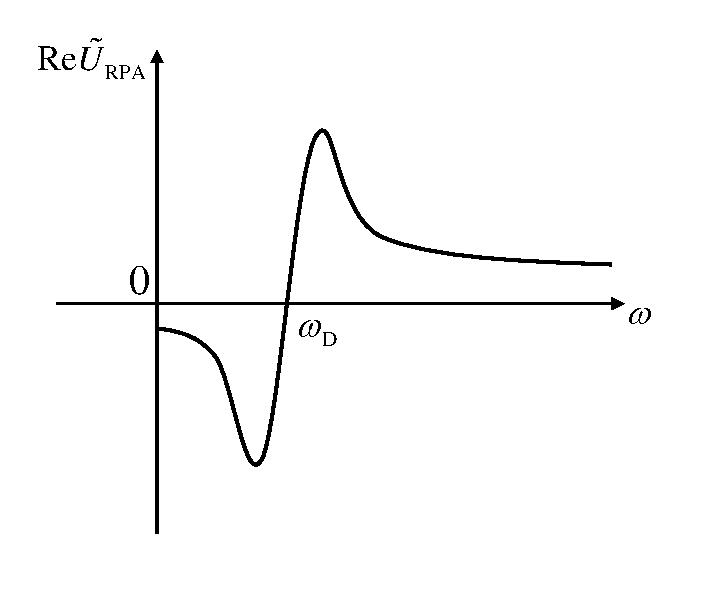
\includegraphics[width=7cm]{figure/RPA1.pdf}
    \caption{有效相互作用势实部随频率变化曲线.}
    \label{U-rpa}
\end{figure}

\subsection{电子-声子系统有效哈密顿量}

前面已经基本分析完了金属体系中, 声子对电子系统的影响. 现在我们要考虑电子-声子相互作用对电子态的影响. 在这里我们不需要从头开始重新计算, 只要选取能突出基本物理的有效哈密顿量即可, 这就是这里讨论有效哈密顿量的原因. 电子-声子系统的有效哈密顿量由三部分组成: 
\begin{equation}
    \hat{H}_{\fun{eff}}=\hat{H}_{\fun{el}}+\hat{H}_{\fun{ph}}+\hat{H}_{\fun{el-ph}},
\end{equation}
其中: 
\begin{equation}
    \hat{H}_{\fun{el}}=\sum_{k\sigma}\ls \frac{k^2\hbar^2}{2m^*}-\mu \rs \hat{c}_{k\sigma}^{\dg}\hat{c}_{k\sigma}^{ },
\end{equation}
\begin{equation}
    \hat{H}_{\fun{ph}}=\sum_q\tilde{\omega}(\vct{q})\ls \hat{a}_q^\dg \hat{a}_q^{ }+\frac{1}{2} \rs,
\end{equation}
\begin{equation}
    \hat{H}_{\fun{el-ph}}=\sum_{k\sigma}\sum_{q\ne 0}g_{\fun{RPA}}(\vct{q})\hat{A}_q^{ }\hat{c}_{k+q,\sigma}^\dg \hat{c}_{k\sigma}^{ },
\end{equation}
考虑进声子相互作用后, 每个子系统哈密顿量都不同于原始哈密顿量. 其中 $\hat{c}_{k\sigma}^\dg$ 和 $\hat{c}_{k\sigma}^{ }$ 是有效电子的产生湮灭算符, 声子频率 $\tilde{\omega}(\vct{q})$ 是前面我们修正过的, 电声耦合 $g_{\fun{RPA}}(\vct{q})$ 也是前面修正过后的结果.

不考虑电子-电子相互作用, 电子自能和声子自能可以分别用费曼图表示为 
$$
    \feyndiagram{
        \vertex[NWblob](a)at(1,0){};
        \vertex[NWblob](b)at(-1,0){};
        \propag[plain](2,0)to(a);
        \propag[plain](a)to(b);
        \propag[plain](b)to(-2,0);
        \propag[bos](a)to[half right, looseness=1.6](b);
        \vertex(c)at(0,0.8){$D_{\fun{RPA}}$};
        \vertex(d)at(0,-1.3){电子自能};
    },\qquad\quad
    \feyndiagram{
        \vertex[NWblob](a)at(0.7,0){};
        \vertex[NWblob](b)at(-0.7,0){};
        \propag[bos](2,0)to(a);
        \propag[plain](a)to[half left, looseness=1.4](b);
        \propag[plain](b)to[half left, looseness=1.4](a);
        \propag[bos](b)to(-2,0);
        \vertex(c)at(1.7,0.4){$D_{\fun{RPA}}$};
        \vertex(c)at(-1.7,0.4){$D_{\fun{RPA}}$};
        \vertex(d)at(0,-1.3){声子自能};
    }.
$$
上述两个修正过的自能图可以用于讨论电子-声子相互作用对金属电阻随温度变化的影响. 

另外, 可以由 Migdal 定理证明关系式: 
\begin{equation}
    \feyndiagram{
        \vertex[NWblob](a)at(0,0){};
        \vertex[NWblob](b)at(-1,-1){};
        \vertex[NWblob](c)at(-1,1){};
        \propag[bos](1.5,0)to(a);
        \propag[plain](a)to(b);
        \propag[plain](a)to(c);
        \propag[plain](b)to(-2,-2);
        \propag[plain](c)to(-2,2);
        \propag[bos](b)to[half left, looseness=1.6](c);
    }
    \propto 
    \sqrt{\frac{m}{M}}\times
    \feyndiagram{
        \vertex[NWblob](a)at(0,0){};
        \propag[bos](1.5,0)to(a);
        \propag[plain](a)to(-1,-1);
        \propag[plain](a)to(-1,1);
    },
\end{equation}
Migdal 这一证明的前提假设也是 $\tilde{\omega_q}\propto c_{\fun{L}}q$, 因此整体来说, 我们在上面给出的推导是自洽的.

\section{Gor'kov 的超导格林函数理论(松原格林函数的应用之三)}
正确的超导理论最早是 1956 年提出的 BCS 理论, 这一套理论虽然成功, 但是它的短板是只能考虑大块的均匀超导体. 当系统具有外磁场等影响时, 这套理论将束手无策. 因此我们非常需要一套能够处理非均匀情况的超导理论. Gor'kov 于 1958 年提出的格林函数的超导理论正是用来描述非均匀超导的一套成功的理论, 其中运用的就是有限温的格林函数. 

在 1950 年左右, 人们提出了一套超导的唯象理论, 即 G-L 理论, 但这一理论的微观基础人们并不明确. Gor'kov 理论从微观的格林函数满足的方程出发, 导出了 G-L 理论满足的方程. 这一做法非常令人惊叹, 这一套理论需要大量推导. 可见 Gor'kov 的物理直觉十分敏锐, 数学功底非常扎实. 希望理论工作的同学们要向老一辈物理学家看齐, 学习他们认真踏实, 坚韧不拔, 严密的工作精神. 

下面我们简单地介绍一下这一理论. 
\subsection{约化哈密顿量及其平均场近似}
约化哈密顿量由两部分构成:
\begin{equation}
    \hat{H}=\hat{H}_0+\hat{H}',\quad \hat{H}_0=\sum_\alpha \int\dd \vct{x}\hat{\psi}_\alpha^{\dg}(\vct{x})\hat{h}(\vct{x})\hat{\psi}_\alpha^{ }(\vct{x}),
\end{equation}
其中 $\hat{h}(\vct{x})$ 是单体算符, 表示为 
\begin{equation}
    \hat{h}(\vct{x})=\frac{\lmi -\ii\nabla-e\vct{A}(\vct{x}) \rmi^2}{2m},
\end{equation}
其中 $\hat{A}(\vct{x})$ 是磁矢势. 在这里还考虑了 London 规范, 即有 
\begin{equation}
    \left\{
        \begin{aligned}
            &\nabla\times\vct{A}=\vct{B},\\
            &\nabla\cdot\vct{A}=0.
        \end{aligned}
    \right.
\end{equation}
在巨正则系综下有 
\begin{equation}
    \hat{h}_\mu(\vct{x})=\hat{h}(\vct{x})-\mu.
\end{equation}

二体相互作用项表示为 
\begin{equation}
    \hat{H}'=\frac{1}{2}\sum_{\alpha\beta}\iint\dd\vct{x}\dd \vct{x}'\hat{\psi}_\alpha^\dg (\vct{x})\hat{\psi}_{\beta}^\dg(\vct{x}')V(\vct{x}-\vct{x}')\hat{\psi}_{\beta}^{ }(\vct{x}')\hat{\psi}_{\alpha}^{ }(\vct{x}).
\end{equation}
这里的相互作用势对超导体来说 $V<0$ 是吸引势. 为简单起见, 我们考虑以下几种简化情况.

(a) 自旋单态超导体 

自旋单态超导体的自旋指标 $\beta=\bar{\alpha}$, 即二体相互作用项可以简化为 
  \begin{align}
        \hat{H}'=&\frac{1}{2}\sum_{\alpha}\iint\dd\vct{x}\dd \vct{x}'\hat{\psi}_\alpha^\dg (\vct{x})\hat{\psi}_{\bar{\alpha}}^\dg(\vct{x}')V(\vct{x}-\vct{x}')\hat{\psi}_{\bar{\alpha}}^{ }(\vct{x}')\hat{\psi}_{\alpha}^{ }(\vct{x})\nonumber\\
        =&\iint\dd\vct{x}\dd\vct{x}'\hat\psi_{\ua}^\dg(\vct{x})\hat\psi_\da^\dg(\vct{x}')V(\vct{x}-\vct{x}')\hat\psi_\da^{ }(\vct{x}')\hat\psi_\ua^{ }(\vct{x}).
    \end{align}

(b) 只考虑 $s$-波情况 

此时只有点接触型相互作用 $V(\vct{x}-\vct{x}')=-g\delta(\vct{x}-\vct{x}')$, 其中 $g>0$. 此时二体相互作用项写为  
\begin{equation}
    \hat{H}'=-g\int\dd\vct{x}\hat{\psi}_\ua^\dg(\vct{x})\hat\psi_\da^\dg(\vct{x})\hat{\psi}_\da^{ }(\vct{x})\hat{\psi}_{\ua}^{ }(\vct{x}),
\end{equation}
这样的场算符四次项难以处理, 下面我们取平均场近似进行计算.

平均场近似的基本假设是 
\begin{equation}
    \llag \hat{\psi}_\ua^\dg(\vct{x})\hat\psi_\da^\dg(\vct{x}) \rrag\ne 0,\quad \llag \hat\psi_\da(\vct{x})\hat\psi_\ua(\vct{x}) \rrag\ne 0.
\end{equation}
将场算符二次项表示为 
\begin{equation}
    \hat{\psi}_{\downarrow}(\vct{x}) \hat{\psi}_{\uparrow}(\vct{x})=\left\langle\hat{\psi}_{\downarrow}(\vct{x}) \hat{\psi}_{\uparrow}(\vct{x})\right\rangle+\left(\hat{\psi}_{\downarrow}(\vct{x}) \hat{\psi}_{\uparrow}(\vct{x})-\left\langle\hat{\psi}_{\downarrow}(\vct{x}) \hat{\psi}_{\uparrow}(\vct{x})\right\rangle\right),
\end{equation}
\begin{equation}
    \hat{\psi}_{\uparrow}^\dg(\vct{x}) \hat{\psi}_{\downarrow}^\dg(\vct{x}) =\left\langle\hat{\psi}_{\uparrow}^\dg(\vct{x}) \hat{\psi}_{\downarrow}^\dg(\vct{x})\right\rangle+\left(\hat{\psi}_{\uparrow}^\dg(\vct{x}) \hat{\psi}_{\downarrow}^\dg(\vct{x})-\left\langle\hat{\psi}_{\uparrow}^\dg(\vct{x}) \hat{\psi}_{\downarrow}^\dg(\vct{x})\right\rangle\right) .
\end{equation}
将括号中的两项视为一阶涨落 $\delta$, 并忽略二阶及以上的小量, 二体相互作用项可以表示为
 \begin{align}
        \hat{H}'= & -g \int \mathrm{d} \vct{x}\left[\left\langle\hat{\psi}_{\uparrow}^\dg(\vct{x}) \hat{\psi}_{\downarrow}^\dg(\vct{x})\right\rangle+\left(\hat{\psi}_{\uparrow}^\dg(\vct{x}) \hat{\psi}_{\downarrow}^\dg(\vct{x})-\left\langle\hat{\psi}_{\uparrow}^\dg(\vct{x}) \hat{\psi}_{\downarrow}^\dg(\vct{x})\right\rangle\right)\right]\nonumber \\
        & \times{\left[\left\langle\hat{\psi}_{\downarrow}(\vct{x}) \hat{\psi}_{\uparrow}(\vct{x})\right\rangle+\left(\hat{\psi}_{\downarrow}(\vct{x}) \hat{\psi}_{\uparrow}(\vct{x})-\left\langle\hat{\psi}_{\downarrow}(\vct{x}) \hat{\psi}_{\uparrow}(\vct{x})\right\rangle\right)\right] } \nonumber\\
        \approx & -g \int \mathrm{d} \vct{x}\left(\left\langle\hat{\psi}_{\uparrow}^\dg(\vct{x}) \hat{\psi}_{\downarrow}^\dg(\vct{x})\right\rangle \hat{\psi}_{\downarrow}(\vct{x}) \hat{\psi}_{\uparrow}(\vct{x})+\hat{\psi}_{\uparrow}^\dg(\vct{x}) \hat{\psi}_{\downarrow}^\dg(\vct{x})\left\langle\hat{\psi}_{\downarrow}(\vct{x}) \hat{\psi}_{\uparrow}(\vct{x})\right\rangle\right.\nonumber\\
        &\qquad\qquad\left.-\left\langle\hat{\psi}_{\uparrow}^\dg(\vct{x}) \hat{\psi}_{\downarrow}^\dg(\vct{x})\right\rangle\left\langle\hat{\psi}_{\downarrow}(\vct{x}) \hat{\psi}_{\uparrow}(\vct{x})\right\rangle\right),
        \end{align}
定义\textbf{对势}(\textbf{pair potential}) $\Delta$:
\begin{equation}
    \left\{
        \begin{aligned}
            &-g\left\langle\hat{\psi}_{\downarrow}(\vct{x}) \hat{\psi}_{\uparrow}(\vct{x})\right\rangle \equiv \Delta(\vct{x}), \\
            &-g\left\langle\hat{\psi}_{\uparrow}^\dg(\vct{x}) \hat{\psi}_{\downarrow}^\dg(\vct{x})\right\rangle \equiv \Delta^*(\vct{x}) ,
        \end{aligned}
    \right.
\end{equation}
通常也称 $\Delta$ 为能隙函数, 此处要注意它不是一个算符. 

这样就可以把平均场哈密顿量表示为
  \begin{align}
        \hat{H}=&\sum_\alpha \int \mathrm{d} \vct{x} \hat{\psi}_\alpha^\dg(\vct{x}) \hat{h}_\mu(\vct{x}) \hat{\psi}_\alpha(\vct{x})+\int \mathrm{d} \vct{x} \Delta^*(\vct{x}) \hat{\psi}_{\downarrow}(\vct{x}) \hat{\psi}_{\uparrow}(\vct{x})\nonumber\\
        &+\int \mathrm{d} \vct{x} \Delta(\vct{x}) \hat{\psi}_{\uparrow}^\dg(\vct{x}) \hat{\psi}_{\downarrow}^\dg(\vct{x})+\int \mathrm{d} \vct{x} \frac{|\Delta(\vct{x})|^2}{g}.
    \end{align}
\subsection{Gor'kov 的超导格林函数}
为求解平均场近似下的哈密顿量, 定义如下单粒子松原格林函数: 
\begin{equation}
    \mathcal{G}_{\alpha\beta}(\vct{x},\tau;\vct{x}',\tau')=-\llag \hat{T}_\tau\lmi \hat{\psi}_{H\alpha}^{ }(\vct{x},\tau)\hat{\psi}_{H\beta}^\dg(\vct{x}',\tau') \rmi \rrag,
\end{equation}
其中场算符是有限温下的海森堡算符: 
\begin{equation}
    \left\{
        \begin{aligned}
            &\hat{\psi}_{H\alpha}^{ }(\vct{x},\tau)=\e^{\hat{K}\tau}\hat\psi_{\alpha}^{ }(\vct{x})\e^{-\hat{K}\tau},\\
            &\hat{\psi}_{H\beta}^{\dg}(\vct{x}',\tau')=\e^{\hat{K}\tau'}\hat{\psi}_{\beta}^{\dg}(\vct{x}')\e^{-\hat{K}\tau'}.
        \end{aligned}
    \right.
\end{equation}
另外, 此处 $\lag\cdots\rag$ 定义为 
\begin{equation}
    \lag\cdots\rag\equiv \frac{\fun{Tr}\lmi \e^{-\beta\hat{K}}\cdots \rmi}{\fun{Tr}\lmi \e^{-\beta\hat{K}} \rmi}.
\end{equation}

超导的核心思想之一在于费米面附近的态密度足够大, 总可以把任意的色散关系在费米面附近线性展开, 这样就和光子的色散关系一致了, 也就是有化学势 $\mu=0$, 粒子数任意变化而不会改变能量. 所以有巨正则系综下的 $\hat{K}\equiv \hat{H}$. 

下面我们分别用运动方程法和有限温下的费曼图技术求解这一单粒子松原格林函数, 导出 Gor'kov 方程.
\subsection{海森伯绘景中的解法(运动方程法)}
首先考虑场算符的时间导数 
 \begin{align}
        \frac{\pt}{\pt\tau}\hat{\psi}_{H\alpha}(\vct{x},\tau)=&\ls\frac{\pt}{\pt\tau}\e^{\hat{K}\tau}\rs \hat{\psi}_{\alpha}(\vct{x})\e^{-\hat{K}\tau}+\e^{\hat{K}\tau}\hat{\psi}_{\alpha}(\vct{x})\ls \frac{\pt}{\pt \tau}\e^{-\hat{K}\tau} \rs\nonumber\\
        =&\hat{K}\e^{\hat{K}\tau}\hat{\psi}_{\alpha}(\vct{x})\e^{-\hat{K}\tau}-\e^{\hat{K}\tau}\hat{\psi}_{\alpha} (\vct{x})\e^{-\hat{K}\tau}\hat{K}\nonumber\\
        =&\lmi \hat{K},\hat{\psi}_{H\alpha}(\vct{x},\tau) \rmi_-,
    \end{align}
代入超导哈密顿量 $\hat{H}$ 的具体表达式并计算对易关系, 有: 
\begin{align}
        \lmi \hat{H},\hat{\psi}_{\alpha}(\vct{x}) \rmi_-=&\sum_{\beta}\int\dd\vct{x}'\lmi \hat{\psi}_{\beta}^\dg(\vct{x}')\hat{h}(\vct{x}')\hat{\psi}_{\beta}^{ }(\vct{x}'),\hat{\psi}_{\alpha}^{ }(\vct{x}) \rmi_- \nonumber\\
&+ \int\dd\vct{x}'\lmi \Delta(\vct{x}')\hat{\psi}_{\alpha}^\dg (\vct{x}')\hat{\psi}_{\bar{\alpha}}^\dg (\vct{x}'),\hat{\psi}_\alpha^{ }(\vct{x}) \rmi_-,
    \end{align}
第一项对易式: 
 \begin{align}
      \sum_{\beta}\int\dd\vct{x}'  \lmi \hat{\psi}_{\beta}^\dg(\vct{x}')\hat{h}(\vct{x}')\hat{\psi}_{\beta}^{ }(\vct{x}'),\hat{\psi}_{\alpha}(\vct{x}) \rmi_-=&\sum_{\beta}\int\dd\vct{x}'\lmi \hat{\psi}_{\beta}^\dg(\vct{x}'),\hat{\psi}_\alpha(\vct{x}) \rmi_- \hat{h}(\vct{x}')\hat{\psi}_\beta^{ }(\vct{x}')\nonumber\\
        =&-\sum_{\beta}\int\dd\vct{x}'\delta_{\alpha\beta}\delta(\vct{x}'-\vct{x})\hat{h}(\vct{x}')\hat{\psi}_{\beta}^{ }(\vct{x}')\nonumber\\
        =&-\hat{h}(\vct{x})\hat{\psi}_{\alpha}^{ }(\vct{x}),
    \end{align}
第二项对易式
 \begin{align}
       \int\dd\vct{x}' \lmi \Delta(\vct{x}')\hat{\psi}_{\alpha}^\dg(\vct{x}')\hat{\psi}_{\bar{\alpha}}^\dg (\vct{x}'), \hat{\psi}_{\alpha}^{ }(\vct{x})\rmi_-=&-\int\dd\vct{x}'\Delta(\vct{x}')\hat{\psi}_{\bar{\alpha}}^\dg(\vct{x}')\ls -\delta(\vct{x}'-\vct{x}) \rs\nonumber\\
        =&-\Delta(\vct{x})\hat{\psi}_{\bar{\alpha}}^\dg(\vct{x}),
    \end{align}
所以有 
\begin{equation}
    \frac{\pt}{\pt\tau}\hat{\psi}_{H\alpha}^{ }(\vct{x},\tau)=-\hat{h}(\vct{x})\hat{\psi}_{H\alpha}^{ }(\vct{x},\tau)-\alpha\Delta(\vct{x})\hat{\psi}_{H\bar{\alpha}}^\dg(\vct{x},\tau).
\end{equation}
类似地, 有
\begin{equation}
    \frac{\pt}{\pt\tau}\hat{\psi}_{H\alpha}^\dg (\vct{x},\tau)=\hat{h}(\vct{x})\hat{\psi}_{H\alpha}^\dg (\vct{x},\tau)+\alpha\Delta^*(\vct{x})\hat{\psi}_{H\bar\alpha}^{ }(\vct{x},\tau).
\end{equation}
格林函数对"时间"的导数就可以写成: 
  \begin{align}
        \frac{\pt}{\pt \tau}\mathcal{G}_{\alpha\alpha}(\vct{x},\tau;\vct{x}',\tau')=&-\delta(\vct{x}-\vct{x}')\delta(\tau-\tau')-\hat{h}(\vct{x})\mathcal{G}_{\alpha\alpha}(\vct{x},\tau;\vct{x}',\tau')\nonumber\\
&+\alpha \Delta(\vct{x})\mathcal{F}_{\bar{\alpha}\alpha}^{\dg}(\vct{x},\tau;\vct{x}',\tau'),
    \end{align}
其中定义了反常格林函数 
\begin{equation}
    \mathcal{F}_{\bar{\alpha}\alpha}^\dg\equiv \llag \hat{T}_\tau \lmi \hat{\psi}_{H\bar \alpha}^\dg(\vct{x},\tau)\hat{\psi}_{H\alpha}^\dg(\vct{x}',\tau') \rmi \rrag,
\end{equation}
其中改变了自旋指标, 这并不影响计算结果. 这一项在正常态费米子体系中等于零, 但在超导体系中可以不等于零. 另外, 反常格林函数与超导能隙函数直接相关, 即有 
\begin{equation}
    \mathcal{F}_{\downarrow\uparrow}^\dg(\vct{x},\tau;\vct{x}',\tau')=\frac{\Delta^*(\vct{x})}{g}.
\end{equation}

下面求解关于 $\mathcal{F}_{\alpha\beta}^\dg$ 的运动方程, 对 $\tau$ 求导有 
\begin{equation}
    \frac{\pt}{\pt\tau}\mathcal{F}_{\bar{\alpha}\alpha}^\dg(\vct{x},\tau;\vct{x}',\tau')=\hat{h}^*(\vct{x})\mathcal{F}_{\bar{\alpha}\alpha}^\dg(\vct{x},\tau;\vct{x}',\tau')+\alpha \Delta^*(\vct{x})\mathcal{G}_{\alpha\alpha}(\vct{x},\tau;\vct{x}',\tau').
\end{equation}
与前面对 $\mathcal{G}_{\alpha\alpha}$ 的时间导数联立, 得到 Gor'kov 方程组:
\begin{equation}
    \left\{
        \begin{aligned}
            &\frac{\pt}{\pt\tau}\mathcal{G}(\vct{x},\tau;\vct{x}',\tau')=-\delta(\vct{x}-\vct{x}')\delta(\tau-\tau')-\hat{h}(\vct{x})\mathcal{G}(\vct{x},\tau;\vct{x}',\tau')+\Delta(\vct{x})\mathcal{F}^\dg(\vct{x},\tau;\vct{x}',\tau'),\\
            &\frac{\pt}{\pt\tau}\mathcal{F}^\dg(\vct{x},\tau;\vct{x}',\tau')=\hat{h}^*(\vct{x})\mathcal{F}^\dg(\vct{x},\tau;\vct{x}',\tau')+\Delta^*(\vct{x})\mathcal{G}(\vct{x},\tau;\vct{x}',\tau').
        \end{aligned}
    \right.
\end{equation}
由于这里的哈密顿量与时间无关, 可以对时间进行傅立叶变换, 得到:
\begin{equation}
    \left\{
    \begin{aligned}
        &\lmi \ii\omega_n-\hat h(\vct{x}) \rmi\mathcal{G}(\vct{x},\vct{x}';\ii\omega_n)+\Delta(\vct{x})\mathcal{F}^\dg (\vct{x},\vct{x}';\ii\omega_n)=\delta(\vct{x}-\vct{x}'),\\
        &\lmi \ii\omega_n+\hat h^*(\vct{x}) \rmi \mathcal{F}^\dg(\vct{x},\vct{x}';\ii\omega_n)+\Delta^*(\vct{x})\mathcal{G}(\vct{x},\vct{x}';\ii\omega_n)=0,
    \end{aligned}
    \right. 
\end{equation}
同样是 Gor'kov 方程.

在无外磁场的情况下, 系统是空间均匀的, 此时哈密顿量只是粒子坐标差的函数. 因此能隙函数 $\Delta$ 成为一个与坐标无关的常数. 方程可以进一步写成 
\begin{equation}
    \left\{
        \begin{aligned}
            &\lmi \ii\omega_n-\xi_k \rmi\mathcal{G}(\vct{k},\ii\omega_n)+\Delta\mathcal{F}^\dg (\vct{k},\ii\omega_n)=\vct{1},\\
            &\lmi \ii\omega_n +\xi_k\rmi\mathcal{F}^\dg (\vct{k},\ii\omega_n)+\Delta^*\mathcal{G}(\vct{k},\ii\omega_n)=0,
        \end{aligned}
    \right.
\end{equation}
其中有 
\begin{equation}
    \xi_k=\frac{\hbar^2 k^2}{2m}-\mu\equiv \epsilon_k^0-\mu.
\end{equation}
从方程组中易解出 
\begin{equation}
    \left\{
        \begin{aligned}
            &\mathcal{G}(\vct{k},\ii\omega_n)=-\frac{\ii\omega_n+\xi_k}{\omega_n^2+E_k^2},\\
            &\mathcal{F}^\dg(\vct{k},\ii\omega_n)=\frac{\Delta^*}{\omega_n^2+E_k^2},
        \end{aligned}
    \right.
\end{equation}
其中: 
\begin{equation}
    E_k^2\equiv \xi_k^2+|\Delta|^2.
\end{equation}
下一小节利用费曼图技术重新推导出这一结果.
\subsection{费曼图法}
考虑相互作用绘景下的松原格林函数及各自的费曼图:
\begin{equation}
    \left\{
        \begin{aligned}
            &\mathcal{G}_{\ua\da}(\vct{x},\tau;\vct{x}',\tau')=-\llag\hat{T}_{\tau}\lmi \hat{\psi}_{I\ua}(\vct{x},\tau)\hat{\psi}_{I\ua}^\dg(\vct{x}',\tau')\hat{S}(\beta,0) \rmi \rrag_{0\fun{C}}:&\feyndiagram{\propag[doublefermion](1,0)to(-1,0);},\\
            &\mathcal{F}_{\da\ua}^\dg (\vct{x},\tau;\vct{x}',\tau')=\llag \hat{T}_\tau\lmi \hat{\psi}_{I\da}^\dg(\vct{x},\tau)\hat{\psi}_{I\ua}^\dg(\vct{x}',\tau')\hat{S}(\beta,0) \rmi \rrag_{0\fun{C}}:&\feyndiagram{\propag[doublefermion](1,0)to(0,0);\propag[doublefermion](-1,0)to(0,0);}.
        \end{aligned}
    \right.
\end{equation}
其中相互作用绘景下的场算符表达式为 
\begin{equation}
    \hat{\psi}_{I\da}^\dg(\vct{x},\tau)=\e^{\hat{H}_0\tau}\hat{\psi}_{\da}^\dg(\vct{x})\e^{-\hat{H}_0\tau},
\end{equation}
有限温下的散射矩阵 $\hat{S}$ 表达式为
\begin{equation}
    \hat{S}(\beta,0)=\hat{T}_\tau\fun{exp}\lmi -\int_0^\beta\hat{H}_I'(\tau')\dd\tau' \rmi,
\end{equation} 
这一项的展开式从二阶项开始.

用单费米线 $\feyndiagram{\propag[fer](0.5,0)to(-0.5,0);}$ 表示自由粒子系统格林函数 $\mathcal{G}^{0}(\vct{x},\tau;\vct{x}',\tau')$, 格林函数的展开式就可以表示为 
   \begin{align}
        \feyndiagram{
            \propag[doublefermion](1,0)to(-1,0);
            \vertex(a)at(0,-0.4){$\vct{k},\ii\omega_n$};
        }
        =\; 
        &
        \feyndiagram{
            \propag[fer](1,0)to(-1,0);
            \vertex(a)at(0,-0.4){$\vct{k},\ii\omega_n$};
        }
        +
        \feyndiagram{
            \propag[fer](-1,0)to(-3,0);
            \propag[fer](-1,0)to(1,0);
            \propag[fer](3,0)to(1,0);
            \propag[sca](-1,0)to(-1,1);
            \propag[sca](1,0)to(1,1);
            \vertex(a)at(1.1,1.1){$\Delta^*$};
            \vertex(b)at(-1,1.1){$\Delta$};
            \vertex(c)at(-2.3,-0.3){$\vct{k},\ii\omega_n$};
            \vertex(d)at(0,-0.3){$ -\vct{k},-\ii\omega_n$};
            \vertex(e)at(2.3,-0.3){$\vct{k},\ii\omega_n$};
        }\nonumber\\
        &+
        \feyndiagram{
            \propag[fer](-3,0)to(-1,0);
            \propag[fer](1,0)to(-1,0);
            \propag[fer](1,0)to(3,0);
            \propag[fer](5,0)to(3,0);
            \propag[fer](-3,0)to(-5,0);
            \propag[sca](-1,0)to(-1,1);
            \propag[sca](1,0)to(1,1);
            \propag[sca](-3,0)to(-3,1);
            \propag[sca](3,0)to(3,1);
            \vertex(a)at(1,1.1){$\Delta$};
            \vertex(b)at(-0.9,1.1){$\Delta^*$};
            \vertex(f)at(-3,1.1){$\Delta$};
            \vertex(g)at(3.1,1.1){$\Delta^*$};
        }\nonumber\\
        &+\cdots,
    \end{align}
回顾前面章节中, 我们用正规自能表示格林函数时有
 \begin{align}
        \feyndiagram{\propag[doublefermion] (0.4,0) to (-0.5,0);}=\; &
        \feyndiagram{\propag[fer] (0.4,0) to (-0.4,0);}
        +
        \feyndiagram{\vertex (a) at (-1,0);\selfnormalsigma{b}{0,0};\vertex (c) at (1,0);\propag[fer](b) to (a);\propag[fer] (c) to (b);}
        +
        \feyndiagram{\vertex (a) at (-1.5,0);\selfnormalsigma{b}{-0.5,0};\selfnormalsigma{c}{0.5,0};\vertex (d) at (1.5,0);\propag[fer] (b) to (a);\propag[plain](c) to (b);\propag[fer](d) to (c);}
        % +
        % \feyndiagram{\vertex (a) at (-1.5,0);\selfnormalsigma{b}{-0.5,0};\selfnormalsigma{c}{0.5,0};\selfnormalsigma{d}{1.5,0};\vertex (e) at (2.5,0);\propag[fer] (b) to (a);\propag[plain](c) to (b);\propag[plain](d) to (c);\propag[fer] (e) to (d);}
        +\cdots\nonumber\\
        =&\feyndiagram{\propag[fer] (0.4,0) to (-0.4,0);}
         +
            \feyndiagram{
            \vertex(a)at(-1,0);
            \selfnormalsigma{b}{0,0};
            \vertex(c)at(1,0);
            \propag[fer](b)to(a);
            \propag[doublefermion](c)to(b);
        },
    \end{align}
可以按照类似的关系来定义超导格林函数的正规自能:
\begin{equation}
    \feyndiagram{
        \propag[fer](-1,0)to(1,0);
        \propag[sca](-1,0)to(-1,1);
        \propag[sca](1,0)to(1,1);
        \vertex(a)at(-1,1.1){$\Delta$};
        \vertex(b)at(1.1,1.1){$\Delta^*$};
    },\quad\Sigma^*\equiv-\frac{|\Delta|^2}{-\ii\omega_n-\xi_{-k}}=\frac{|\Delta|^2}{\ii\omega_n+\xi_k},
\end{equation}
从而得到格林函数 
\begin{equation}
    \mathcal{G}(\vct{k},\ii\omega_n)=\frac{1}{\ii\omega_n-\xi_k-\frac{|\Delta|^2}{\ii\omega_n+\xi_k}}=-\frac{\ii\omega_n+\xi_k}{\omega_n^2+E_k^2},
\end{equation}
这一结果与前一节的计算结果一致. 

类似地, 有反常格林函数的费曼图展开式 
  \begin{align}
        \feyndiagram{
            \propag[doublefermion](1,0)to(0,0);
            \propag[doublefermion](-1,0)to(0,0);
            }
            =\;&
            \feyndiagram{
                \propag[fer](-1,0)to(0,0);
                \propag[fer](1,0)to(0,0);
                \propag[sca](0,0)to(0,1);
                \vertex(a)at(0.1,1.1){$\Delta^*$};
            }
            +
            \feyndiagram{
                \propag[fer](-2,0)to(-1,0);
                \propag[fer](0,0)to(-1,0);
                \propag[fer](0,0)to(1,0);
                \propag[fer](2,0)to(1,0);
                \propag[sca](-1,0)to(-1,1);
                \propag[sca](0,0)to(0,1);
                \propag[sca](1,0)to(1,1);
                \vertex(a)at(-0.9,1.1){$\Delta^*$};
                \vertex(b)at(0,1.1){$\Delta$};
                \vertex(c)at(1.1,1.1){$\Delta^*$};
            }
            +\cdots\nonumber\\
            =\;&
            \feyndiagram{
                \propag[fer](-1,0)to(0,0);
                \propag[doublefermion](1,0)to(0,0);
                \propag[sca](0,0)to(0,1);
                \vertex(a)at(0.1,1.1){$\Delta^*$};
            },
    \end{align}
解出反常格林函数为 
\begin{equation}
    \mathcal{F}^\dg(\vct{k},\ii\omega_n)=\frac{\Delta^*}{-\ii\omega_n-\xi_k}\ls -\frac{\ii\omega_n+\xi_k}{\omega_n^2+E_k^2} \rs=\frac{\Delta^*}{\omega_n^2+E_k^2}.
\end{equation}

费曼图形式的方程组:
\begin{equation}
    \left\{
    \begin{aligned}
        &\feyndiagram{
            \propag[doublefermion](0.6,0)to(-0.6,0);
        }
        =\;
        \feyndiagram{
            \propag[fer](1,0)to(-1,0);
        }
        +
        \feyndiagram{
            \propag[fer](0,0)to(-1,0);
            \propag[doublefermion](1.2,0)to(0.6,0);
            \propag[doublefermion](0,0)to(0.6,0);
            \propag[sca](0,0)to(0,1);
            \vertex(a)at(0.1,1.1){$\Delta^*$};
        },\\
        &\feyndiagram{
            \propag[doublefermion](-0.6,0)to(0,0);
            \propag[doublefermion](0.6,0)to(0,0);
        }
        =
        \feyndiagram{
            \propag[fer](-1,0)to(0,0);
            \propag[doublefermion](1,0)to(0,0);
            \propag[sca](0,0)to(0,1);
            \vertex(a)at(0.1,1.1){$\Delta^*$};
        },
    \end{aligned}
    \right.
\end{equation}
亦即 Gor'kov 方程.

对超导格林函数变形:
 \begin{align}
        \mathcal{G}(\vct{k},\ii\omega_n)&=-\frac{\ii\omega_n+\xi_k}{\omega_n^2+E_k^2}\nonumber\\
        &=\frac{u_k^2}{\ii\omega_n-E_k}+\frac{v_k^2}{\ii\omega_n+E_k}\nonumber\\
        &\equiv \int_{-\infty}^{\infty}\frac{A(\vct k,\omega')}{\ii\omega_n-\omega'}\dd\omega',
    \end{align}
其中有 
\begin{equation}
    \left\{
        \begin{aligned}
            &u_k^2=\frac{1}{2}\left( 1+\frac{\xi_k}{E_k} \right),\\
            &v_k^2=\frac{1}{2}\left( 1-\frac{\xi_k}{E_k} \right),
        \end{aligned}
    \right.
\end{equation}
并且有关系式 $u_k^2+v_k^2=1$. 另外, 谱函数 $A(\vct{k},\omega)$ 的表达式为 
\begin{equation}
    A(\vct{k},\omega)=u_k^2\delta(\omega-E_k)+v_k^2\delta(\omega+E_k),
\end{equation}
格林函数的正极点对应着准粒子的能量, 有 
\begin{equation}
    E_k=\sqrt{\xi_k^2+|\Delta|^2},
\end{equation}
其中有
\begin{equation}
    \xi_k=\frac{k^2}{2m}-E_{\fun{F}},
\end{equation}
当 $k=k_{\fun{F}}$ 时上式取最小值, 在 $\mu=E_{\fun{F}}$ 时这一结果符合弱耦合理论. 这时 $E_k=|\Delta|$ 称为能隙, 即激发准粒子需要的最小能量.

反常格林函数也可以表示为 
  \begin{align}
        \mathcal{F}^\dg(\vct{k},\ii\omega_n)=&\frac{\Delta^*}{\omega_n^2+E_k^2}\nonumber\\
        =&-\frac{\Delta^*}{2E_k}\ls \frac{1}{\ii\omega_n-E_k}-\frac{1}{\ii\omega_n+E_k} \rs,
    \end{align}
\subsection{物理量的计算}
(a) 能隙方程 

对于大块的超导体, 我们可以选取 $\Delta$ 为实数, 能隙函数可以表示为 
\begin{equation}
    \Delta^*=g\mathcal{F}^\dg(0,-\eta),
\end{equation}
考虑反常格林函数的傅立叶变换 
\begin{equation}
    \mathcal{F}^\dg(\vct{x}-\vct{x}';\tau-\tau')=\int\frac{\dd\vct
    k}{(2\pi)^3}\frac{1}{\beta}\sum_{\omega_n}\e^{\ii\vct{k}\cdot(\vct{x}-\vct{x}')}\e^{-\ii\omega_n(\tau-\tau')}\mathcal{F}^\dg(\vct{k},\ii\omega_n),
\end{equation}
取 $\tau'=\tau+\eta$, $\vct{x}'=\vct{x}$, 就有 
\begin{equation}
    \mathcal{F}^\dg(0,-\eta)=\int\frac{\dd\vct
    k}{(2\pi)^3}\frac{1}{\beta}\sum_{\omega_n}\e^{\ii\omega_n\eta}\mathcal{F}^\dg(\vct{k},\ii\omega_n).
\end{equation}
能隙函数就可以表示成 
  \begin{align}
        \Delta^*&=g\int\frac{\dd\vct
        k}{(2\pi)^3}\frac{1}{\beta}\sum_{\omega_n}\e^{\ii\omega_n\eta}\lmi -\frac{\Delta^*}{2E_k}\ls \frac{1}{\ii\omega_n-E_k}-\frac{1}{\ii\omega_n+E_k} \rs \rmi\nonumber\\
        &=-g\int\frac{\dd\vct{k}}{(2\pi)^3}\ls \frac{1}{\beta}\sum_{\omega_n}\frac{\e^{\ii\omega_n\eta}}{\ii\omega_n-E_k}-\frac{1}{\beta}\sum_{\omega_n}\frac{\e^{\ii\omega_n\eta}}{\ii\omega_n+E_k} \rs\frac{\Delta^*}{2E_k}\nonumber\\
        &=-g\int\frac{\dd\vct{k}}{(2\pi)^3}\lmi n_{\fun{F}}(E_k)-n_{\fun{F}}(-E_k) \rmi\frac{\Delta^*}{2E_k}\nonumber\\
        &=g\Delta^*\int\frac{\dd\vct{k}}{(2\pi)^3}\frac{\tanh\ls \frac{\beta E_k}{2} \rs}{2E_k},
    \end{align}
即有 
\begin{equation}
    1=g\int\frac{\dd\vct{k}}{(2\pi)^3}\frac{\tanh\ls \frac{\beta E_k}{2} \rs}{2E_k},
\end{equation}
其中 $g$ 是电子-声子相互作用的强度. 由于声子只会导致费米面附近的电子有相互吸引作用, 能隙对动量的积分就可以用对能量的积分乘以态密度来代替, 考虑表征声子能量的德拜频率 $\omega_{\fun{D}}$, 就有 
 \begin{align}
        1=&g\int\dd\xi_k N(\xi_k)\frac{\tanh\ls \frac{\beta E_k}{2} \rs}{2\sqrt{\xi_k^2+\Delta^2}} \nonumber \\
        \approx&N(0)g\int_{-\omega_{\fun{D}}}^{\omega_{\fun{D}}}\dd\xi_k\frac{\tanh\ls \frac{\beta E_k}{2} \rs}{2 E_k},
    \end{align}
最后就得到了能隙方程 
\begin{equation}
    1=N(0)g\int_0^{\omega_{\fun{D}}}\dd\xi_k\frac{\tanh\ls \frac{\beta E_k}{2} \rs}{E_k}.
\end{equation}

令 $T=T_{\fun{C}}$, 求解方程得到 
\begin{equation}
    T_{\fun{C}}=1.13\omega_{\fun{D}}\exp\lmi -\frac{1}{gN(0)} \rmi.
\end{equation}

令 $T=0$, 得到 
\begin{equation}
    \Delta(0)=2\omega_{\fun{D}}\exp\lmi -\frac{1}{gN(0)} \rmi,
\end{equation}
并且得到普适关系式 
\begin{equation}
    \frac{2\Delta(0)}{T_{\fun{C}}}=3.53.
\end{equation}

当 $T\ll T_{\fun{C}}$ 时, 有 
\begin{equation}
    \Delta(T)\approx \Delta(0)-\sqrt{ 2\pi T\Delta(0) } \e^{-\Delta(0)/T}.
\end{equation}

当 $T_{\fun{C}}-T\ll T_{\fun{C}}$ 时, 有 
\begin{equation}
    \Delta(T)\approx 3.06 T_{\fun{C}}\ls 1-\frac{T}{T_{\fun{C}}} \rs.
\end{equation}

(b) 热力学势的计算 

前面得到, 热力学势的表达式为
\begin{equation}
    \Omega =\Omega_0+\int_0^1\frac{\dd\lambda}{\lambda}\lag \lambda \hat{H}' \rag_{\lambda},
\end{equation}
其中 
\begin{equation}
    \hat{H}'=-g\int\dd\vct{x}\hat{\psi}^\dg_\ua (\vct{x})\hat{\psi}^\dg_{\da}(\vct{x})\hat{\psi}^{ }_{\da}(\vct{x})\hat{\psi}^{ }_{\ua}(\vct{x}),
\end{equation}
令 $\lambda g\equiv g'$, 并取平均场近似, 得到 
 \begin{align}
        \lambda \hat{H}'=&-g'\int\dd\vct{x}\llag \hat{\psi}_{\ua}^\dg (\vct{x})\hat{\psi}_{\da}^\dg (\vct{x}) \rrag_{g'} \hat{\psi}_{\da}^{ }(\vct{x})\hat{\psi}_{\ua}^{ }(\vct{x})\nonumber\\
        &-g'\int\dd\vct{x}\hat{\psi}_{\ua}^\dg (\vct{x})\hat{\psi}_{\da}^\dg (\vct{x})\llag \hat{\psi}_{\da}^{ }(\vct{x})\hat{\psi}_{\ua}^{ }(\vct{x}) \rrag_{g'}\nonumber\\
        &+g'\int\dd\vct{x}\llag \hat{\psi}_{\ua}^\dg(\vct{x}) \hat{\psi}_{\da}^{\dg}(\vct{x}) \rrag_{g'}\llag \hat{\psi}_\da(\vct{x})\hat{\psi}_{\ua}(\vct{x})  \rrag_{g'},
    \end{align}
对上式再取一次平均值, 就有 
 \begin{align}
        \llag \lambda \hat{H}' \rrag_{\lambda} &=-g'\int\dd\vct{x}\llag \hat{\psi}_\ua^\dg(\vct{x})\hat{\psi}_\da^\dg(\vct{x}) \rrag_{g'} \llag \hat{\psi}_\da^{ }(\vct{x})\hat{\psi}_{\ua}^{ }(\vct{x}) \rrag_{g'}\nonumber\\
        &=-\int\frac{|\Delta_{g'}|^2}{g'}\dd\vct{x}\nonumber\\
        &=-V\frac{|\Delta_{g'}|^2}{g'},
    \end{align}
其中, 由于前面设 $\Delta_{g'}$ 为实数, 所以此处有 $\Delta_{g'}=\Delta^*_{g'}$. 热力学势可以表示为 
  \begin{align}
        \Delta\Omega=&-V\int_0^1\frac{\dd\lambda}{\lambda}\frac{|\Delta_{g'}|^2}{g'}\nonumber\\
        =&-V\int_0^g\frac{\dd g'}{g'}\frac{\Delta^2_{g'}}{g'}\nonumber\\
        =&V\int_0^\Delta \dd\Delta_{g'}\frac{\dd\ls \frac{1}{g'} \rs}{\dd\Delta_{g'}}\Delta^2_{g'},
    \end{align}
根据前面得到的能隙方程, 有 
\begin{equation}
    \frac{1}{g'}=N(0)\int_0^{\omega_{\fun{D}}}\dd\xi_k\lmi \frac{\tanh \ls \frac{\beta\sqrt{\xi_k^2+\Delta_{g'}^2}}{2} \rs }{\sqrt{\xi_k^2+\Delta_{g'}^2}} \rmi,
\end{equation}
代入热力学势表达式中, 就得到 
  \begin{align}
        \frac{\Delta \Omega}{V}=&\int_0^\Delta \Delta^2_{g'}\frac{\dd}{\dd\Delta_{g'}}\lmi N(0)\int_0^{\omega_{\fun{D}}}\dd\xi_k \frac{1}{\sqrt{\xi_k^2+\Delta_{g'}^2}}\tanh\ls \frac{\beta\sqrt{\xi_k^2+\Delta^2_{g'}}}{2} \rs \rmi \dd\Delta_{g'}\nonumber\\
        =&\Delta^2_{g'}N(0)\int_0^{\omega_{\fun{D}}}\frac{1}{\sqrt{\xi_k^2+\Delta_{g'}^2}}\tanh\ls \frac{\beta\sqrt{\xi_k^2+\Delta_{g'}^2}}{2} \rs \dd\xi_k\nonumber\\
        &-2N(0)\int_0^{\omega_{\fun{D}}}\dd\xi_k \lmi \int_0^{\Delta_{g'} }\frac{\Delta_{g'}\dd\Delta_{g'}}{\sqrt{\xi_k^2+\Delta_{g'}^2}}\tanh\ls \frac{\beta\sqrt{\xi_k^2+\Delta_{g'}^2}}{2} \rs \rmi. 
    \end{align}
将 $\Omega-\Omega_0$ 视为自由能的增量, 得到表达式 
  \begin{align}
        \frac{\Omega-\Omega_0}{V}=&\frac{\Delta^2(\tau)}{g}-\frac{4N(0)}{\beta}\int_0^{\omega_{\fun{D}}}\dd\xi_k\fun{ln}\left| \frac{\cosh\ls \frac{\beta E_k}{2} \rs}{\cosh\ls \frac{\beta\xi_k}{2} \rs} \right|\nonumber\\
        =&-\frac{1}{2}N(0)\Delta^2(\tau)-N(0)\Delta^2(\tau)\ln \left| \frac{\Delta(0)}{\Delta(\tau)} \right|\nonumber\\
        &-4N(0)\frac{1}{\beta}\int_0^{\omega_{\fun{D}}}\dd\xi\ln\left| 1+\e^{\beta E_k} \right| +\frac{N(0)}{3}\frac{\pi^2}{\beta^2}.
    \end{align}

利用自由能可以得到比热的普适关系 
\begin{equation}
    \ls \frac{C_{\fun{S}}-C_{\fun{N}}}{C_{\fun{N}}} \rs_{T_{\fun{C}}}=1.43,
\end{equation}
其中超导比热 $C_{\fun{S}}\propto \e^{-\Delta(0)\beta}$ 呈指数衰减. 如图 \ref{sc1} 所示.
\begin{figure}[htbp]
    \centering
    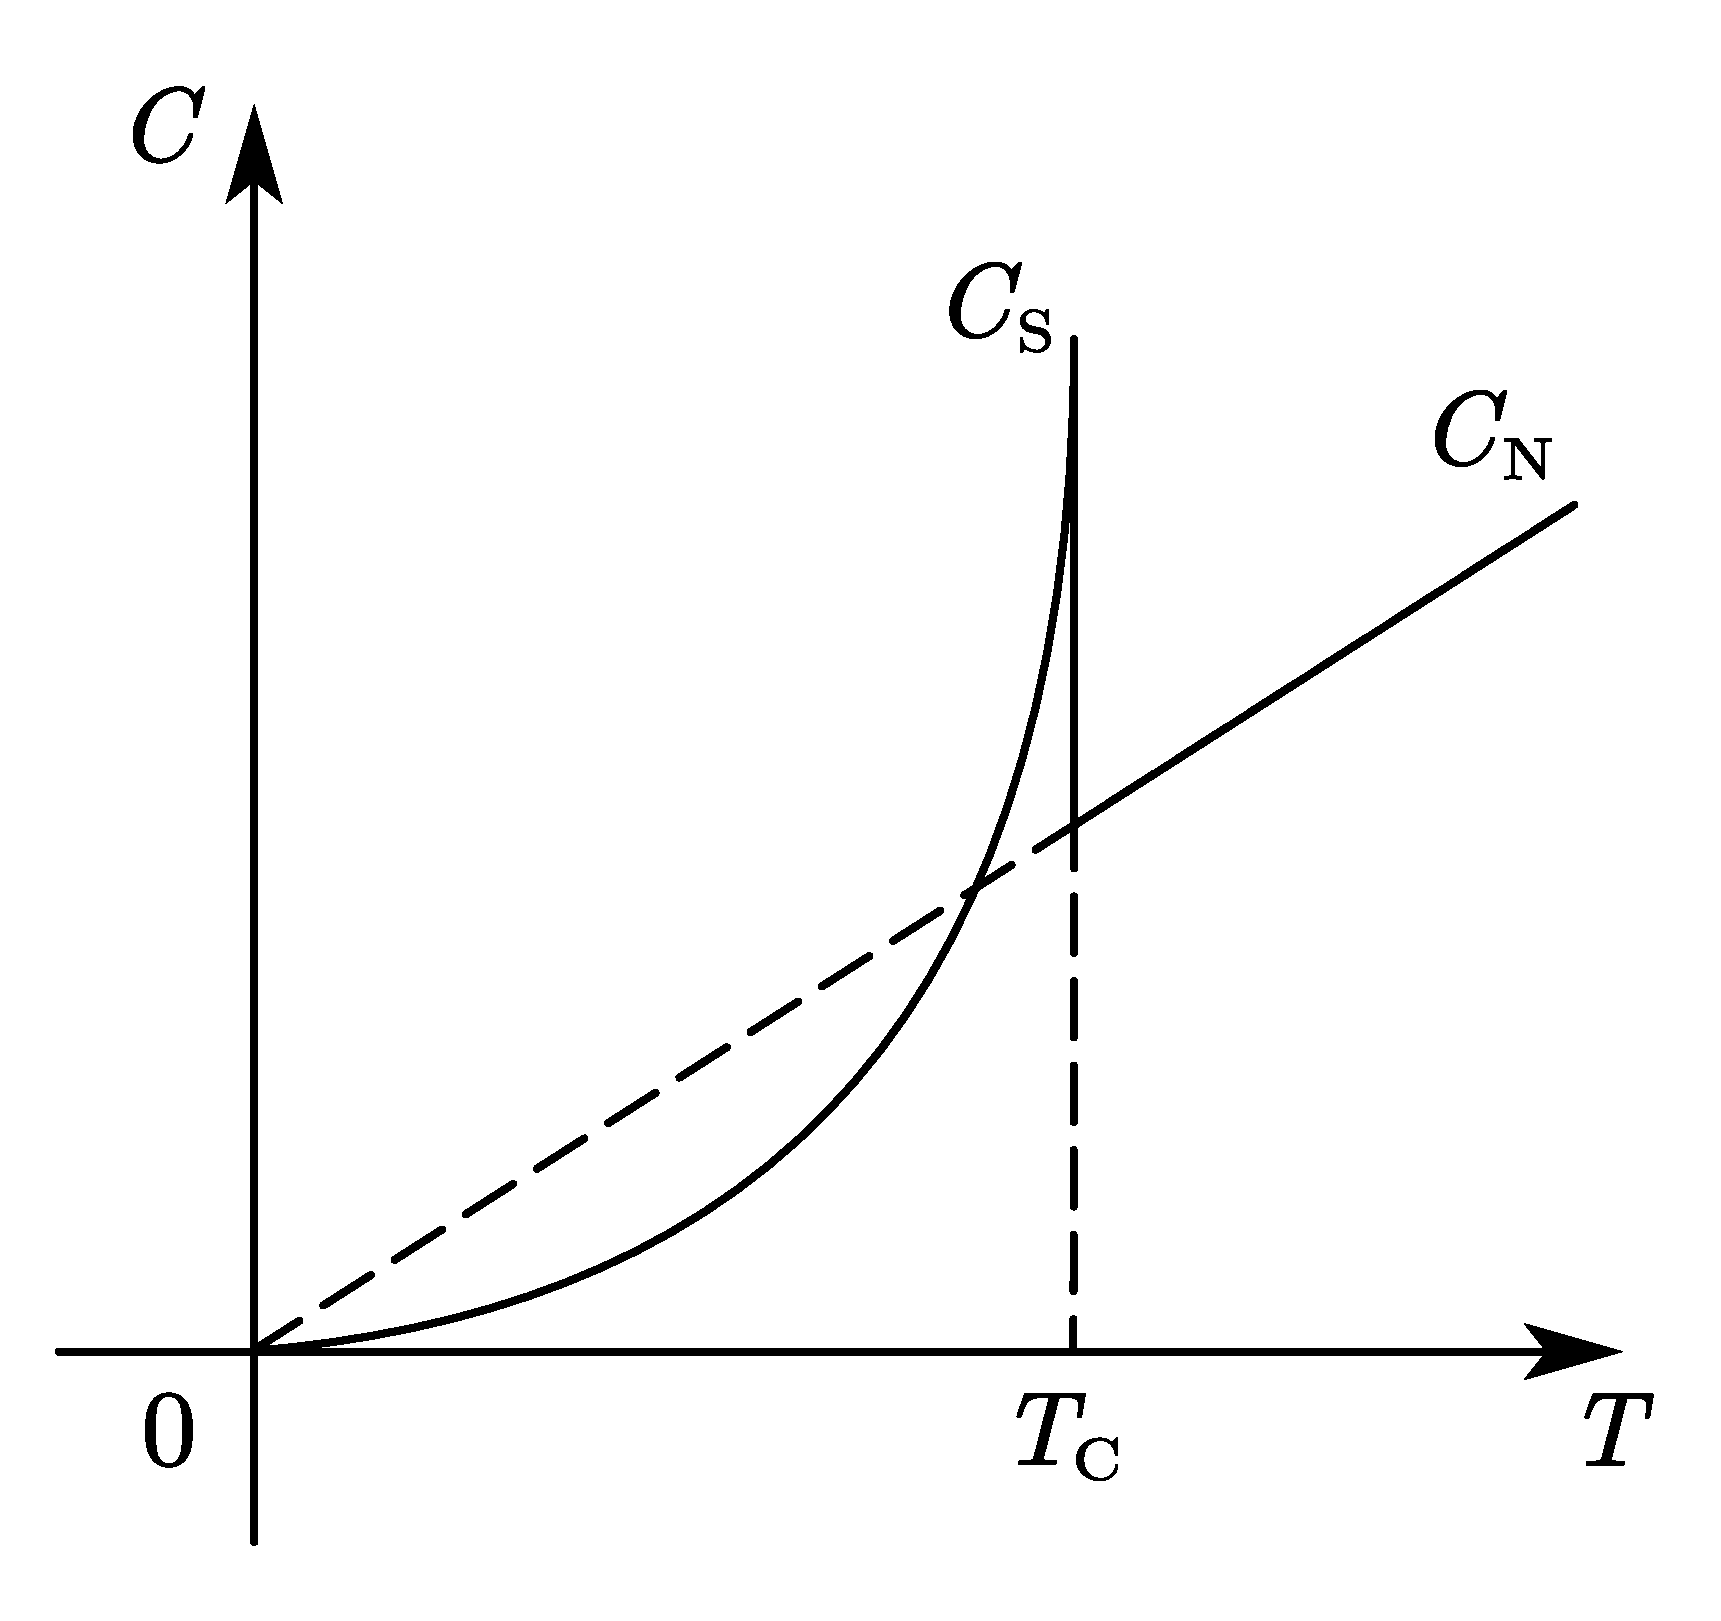
\includegraphics[width=6cm]{figure/sc1.pdf}
    \caption{超导电子比热.}
    \label{sc1}
\end{figure}

临界磁场具有表达式
\begin{equation}
    \left\{
        \begin{aligned}
            &H_{\fun{C}}(T)=H_{\fun{C}}(0)\lmi 1-1.06\ls \frac{T}{T_{\fun{C}}} \rs^2 \rmi,\quad (T\ll T_{\fun{C}}),\\
            &H_{\fun{C}}(T)=1.74 H_{\fun{C}}(0)\ls 1-\frac{T}{T_{\fun{C}}} \rs,\quad (T_{\fun{C}}-T\ll T_{\fun{C}}),
        \end{aligned}
    \right.
\end{equation}
这与 BCS 理论给出的结果一致, 如图 \ref{sc2} 所示.
\begin{figure}[htbp]
    \centering
    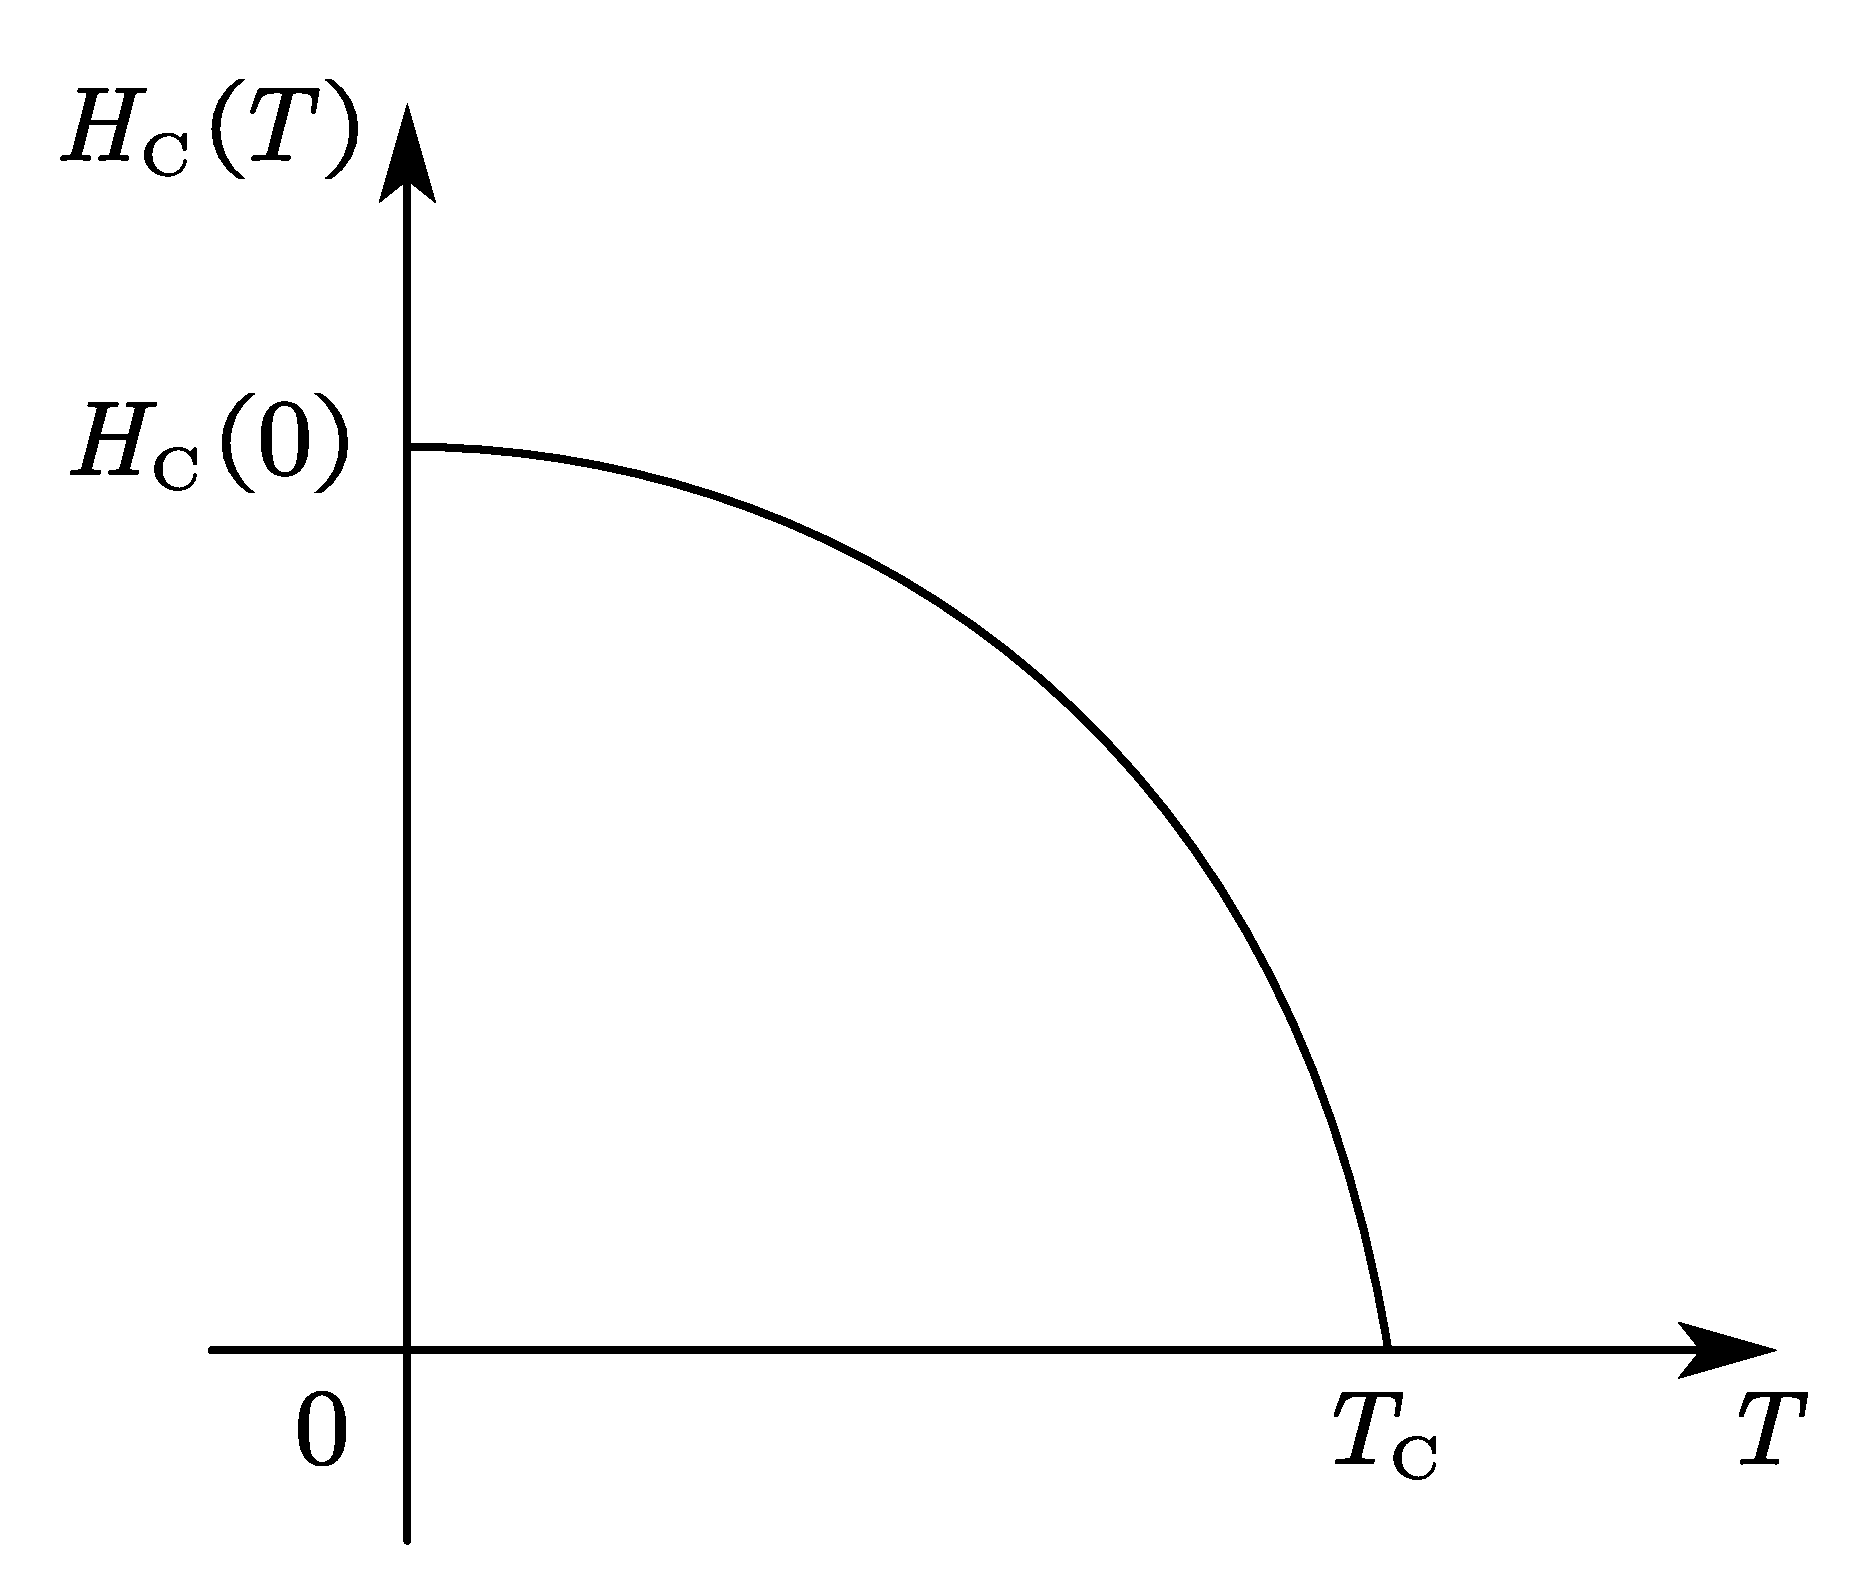
\includegraphics[width=6.5cm]{figure/sc2.pdf}
    \caption{超导电子临界磁场随温度变化.}
    \label{sc2}
\end{figure}

(c) 超导电子动量分布与态密度

计算超导电子的粒子数期望值:
 \begin{align}
        \lag\hat{N}\rag=&2V\frac{1}{\beta}\sum_{\omega_n}\int\frac{\dd\vct{k}}{(2\pi)^3}\mathcal{G}(\vct{k},\ii\omega_n)\e^{\ii\omega_n\eta}\nonumber\\
        =&2V\frac{1}{\beta}\sum_{\omega_n}\int\frac{\dd\vct{k}}{(2\pi)^3}\ls \frac{u_k^2}{\ii\omega-E_k}+\frac{v_k^2}{\ii\omega+E_k} \rs\e^{\ii\omega_n\eta}\nonumber\\
        =&2V\int\frac{\dd\vct{k}}{(2\pi)^3}\lmi u_k^2n_{\fun{F}}(E_k)+v_k^2n_{\fun{F}}(-E_k) \rmi\nonumber\\
        =&2\sum_k\lmi u_k^2n_{\fun{F}}(E_k)+v_k^2n_{\fun{F}}(-E_k) \rmi,
    \end{align}
其中费米分布的表达式为 
\begin{equation}
    n_{\fun{F}}(E_k)=\frac{1}{\e^{\beta E_k}+1},
\end{equation}
设粒子数分布与自旋指标无关, 则算符和期望值可以在形式上表示成 
\begin{equation}
    \hat{N}=\sum_{k\sigma}\hat{C}_{k\sigma}^\dg \hat{C}_{k\sigma}^{ },\quad \lag \hat{N} \rag=\sum_{k\sigma}\lag \hat{C}_{k\sigma}^\dg \hat{C}_{k\sigma}^{ } \rag=2\sum_k\lag \hat{C}_k^\dg \hat{C}_k^{ } \rag,
\end{equation}
令 
\begin{equation}
    \lag \hat{C}_k^\dg \hat{C}_k^{ } \rag\equiv n_k,
\end{equation}
就得到超导电子的动量分布为 
\begin{equation}
    n_k=u_k^2 n_{\fun{F}}(E_k)+v_k^2n_{\fun{F}}(-E_k).
\end{equation}
当 $T=0$ 时, 有 $n_k=v_k^2$. 在超导电子的动量分布中, 超导态的电子会增加动能, 但是 Cooper pair 的势能减少得更多. 这是一种与 Pauli 不相容原理相关的多体关联效应. 超导电子的动量分布如图 \ref{sc3} 所示.
\begin{figure}[htbp]
    \centering
    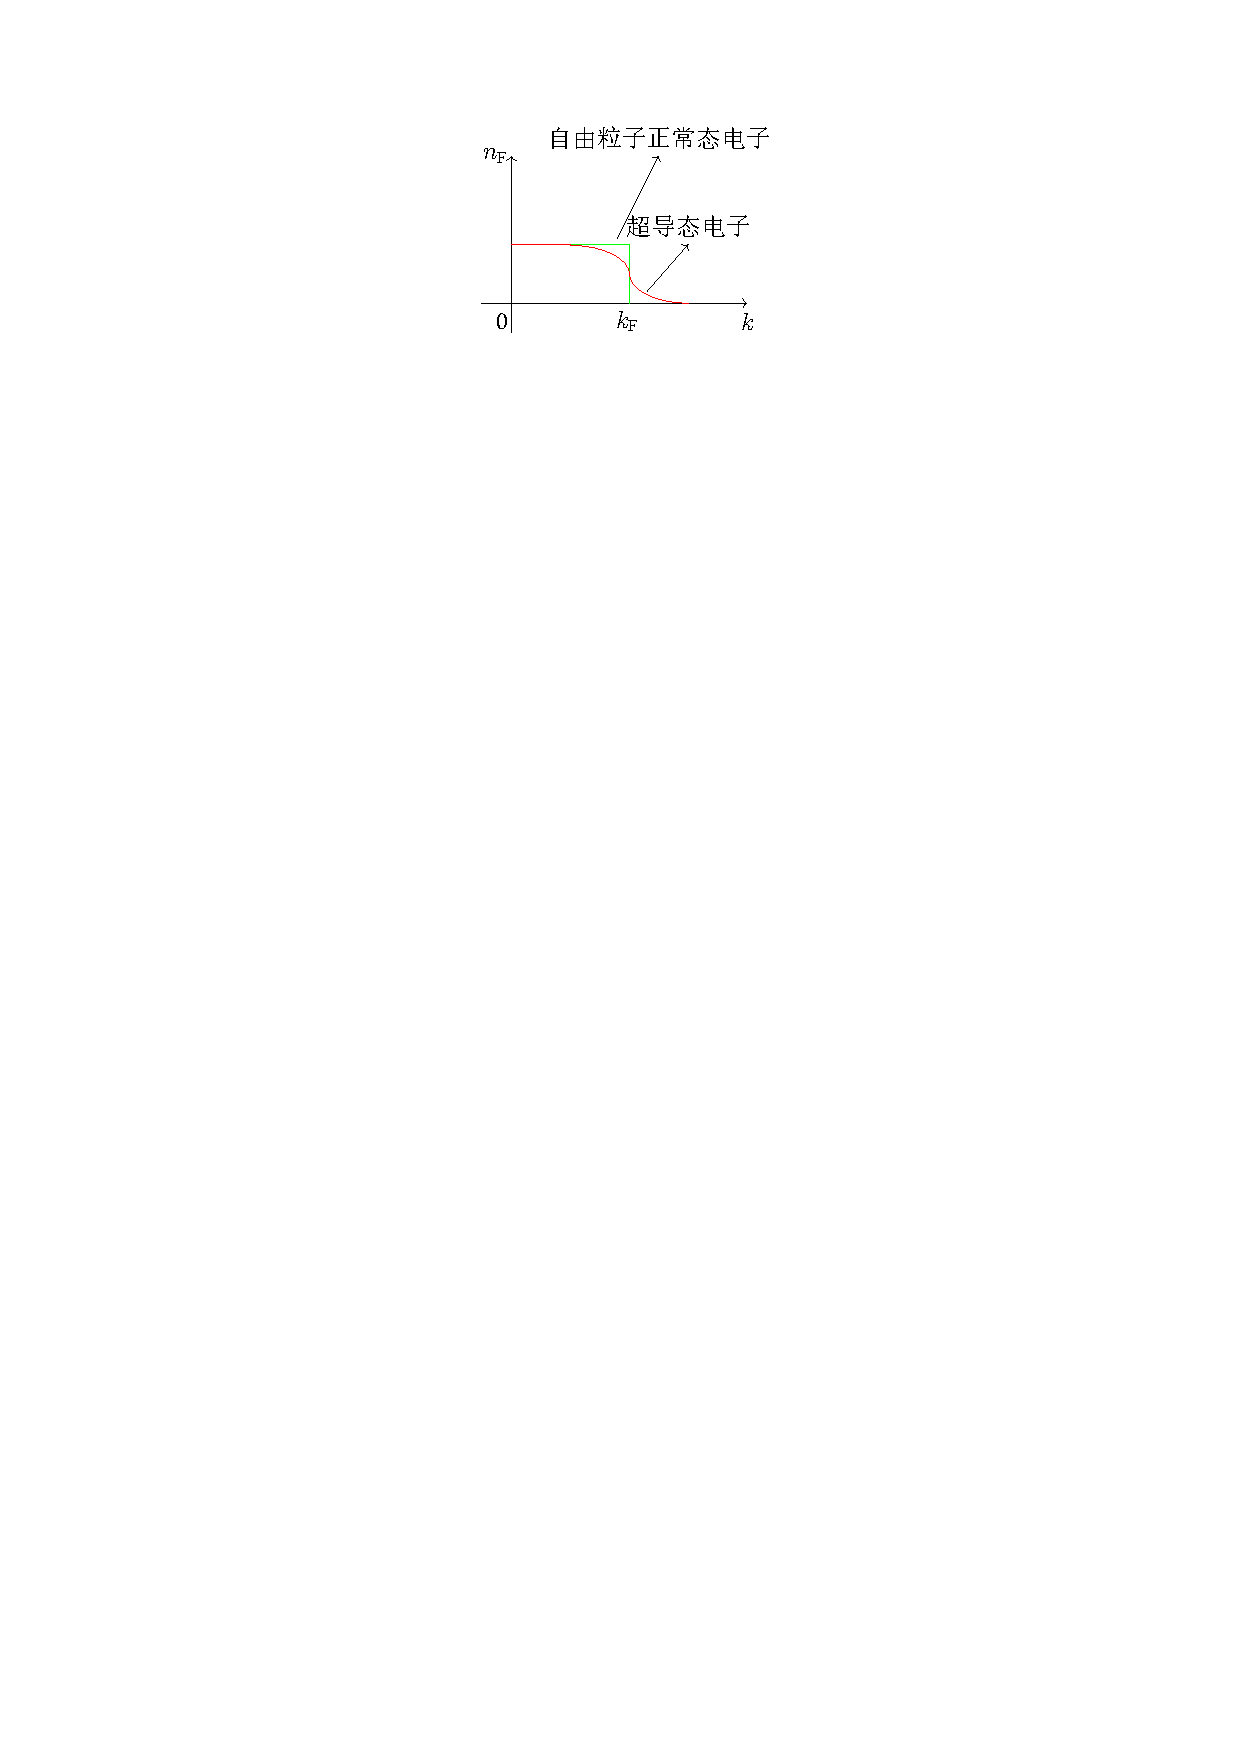
\includegraphics[width=6.5cm]{figure/sc3.pdf}
    \caption{超导电子的动量分布.}
    \label{sc3}
\end{figure}

重新将 $\lag N \rag$ 变形, 有 
 \begin{align}
        \lag N \rag=&2V\int\frac{\dd\vct{k}}{(2\pi)^3}\lmi u_k^2 n_{\fun{F}}(E_k)+v_{\fun{F}}^2n_{\fun{F}}(-E_k) \rmi\nonumber\\
        =&2\int\dd\omega n_{\fun{F}}(\omega)\sum_k\lmi u_k^2\delta(\omega-E_k)+v_k^2\delta(\omega+E_k) \rmi\nonumber\\
        \equiv &2\int\dd\omega n_{\fun{F}}(\omega)N_{\fun{S}}(\omega),
    \end{align}
其中 $N_{\fun{S}}(\omega)$ 的物理意义是 $\omega$ 态粒子的态密度, 表达式可以写成 
  \begin{align}
        N_{\fun{S}}(\omega)=&\sum_k\lmi u_k^2\delta(\omega-E_k)+v_{k}^2\delta(\omega+E_k) \rmi\nonumber\\
        =&\sum_k A(\vct{k},\omega),
    \end{align}
其中谱函数 $A(\vct{k},\omega)$ 与推迟格林函数有直接联系: 
\begin{equation}
    A(\vct{k},\omega)=-\frac{1}{\pi}\fun{Im}G^{R}(\vct{k},\ii\omega),
\end{equation}
所以电子态密度可以表示成 
\begin{equation}
    N_{\fun{S}}(\vct{k})=\sum_k -\frac{1}{\pi} \fun{Im}G^R(\vct{k},\ii\omega),
\end{equation}
根据松原格林函数和热力学推迟格林函数之间的关系, 可以直接得到推迟格林函数的表达式 
 \begin{align}
        \mathcal{G}(\vct{k},\ii\omega_n\to \omega+\ii\eta)=&G^R(\vct{k},\omega)\nonumber\\
        =&\frac{u_k^2}{\omega-E_k+\ii\eta}+\frac{v_k^2}{\omega+E_k+\ii\eta}.
    \end{align}
超导电子态密度分布如图 \ref{sc4} 所示, 这一结果与实验测得结果一致.

\begin{figure}[htbp]
    \centering
    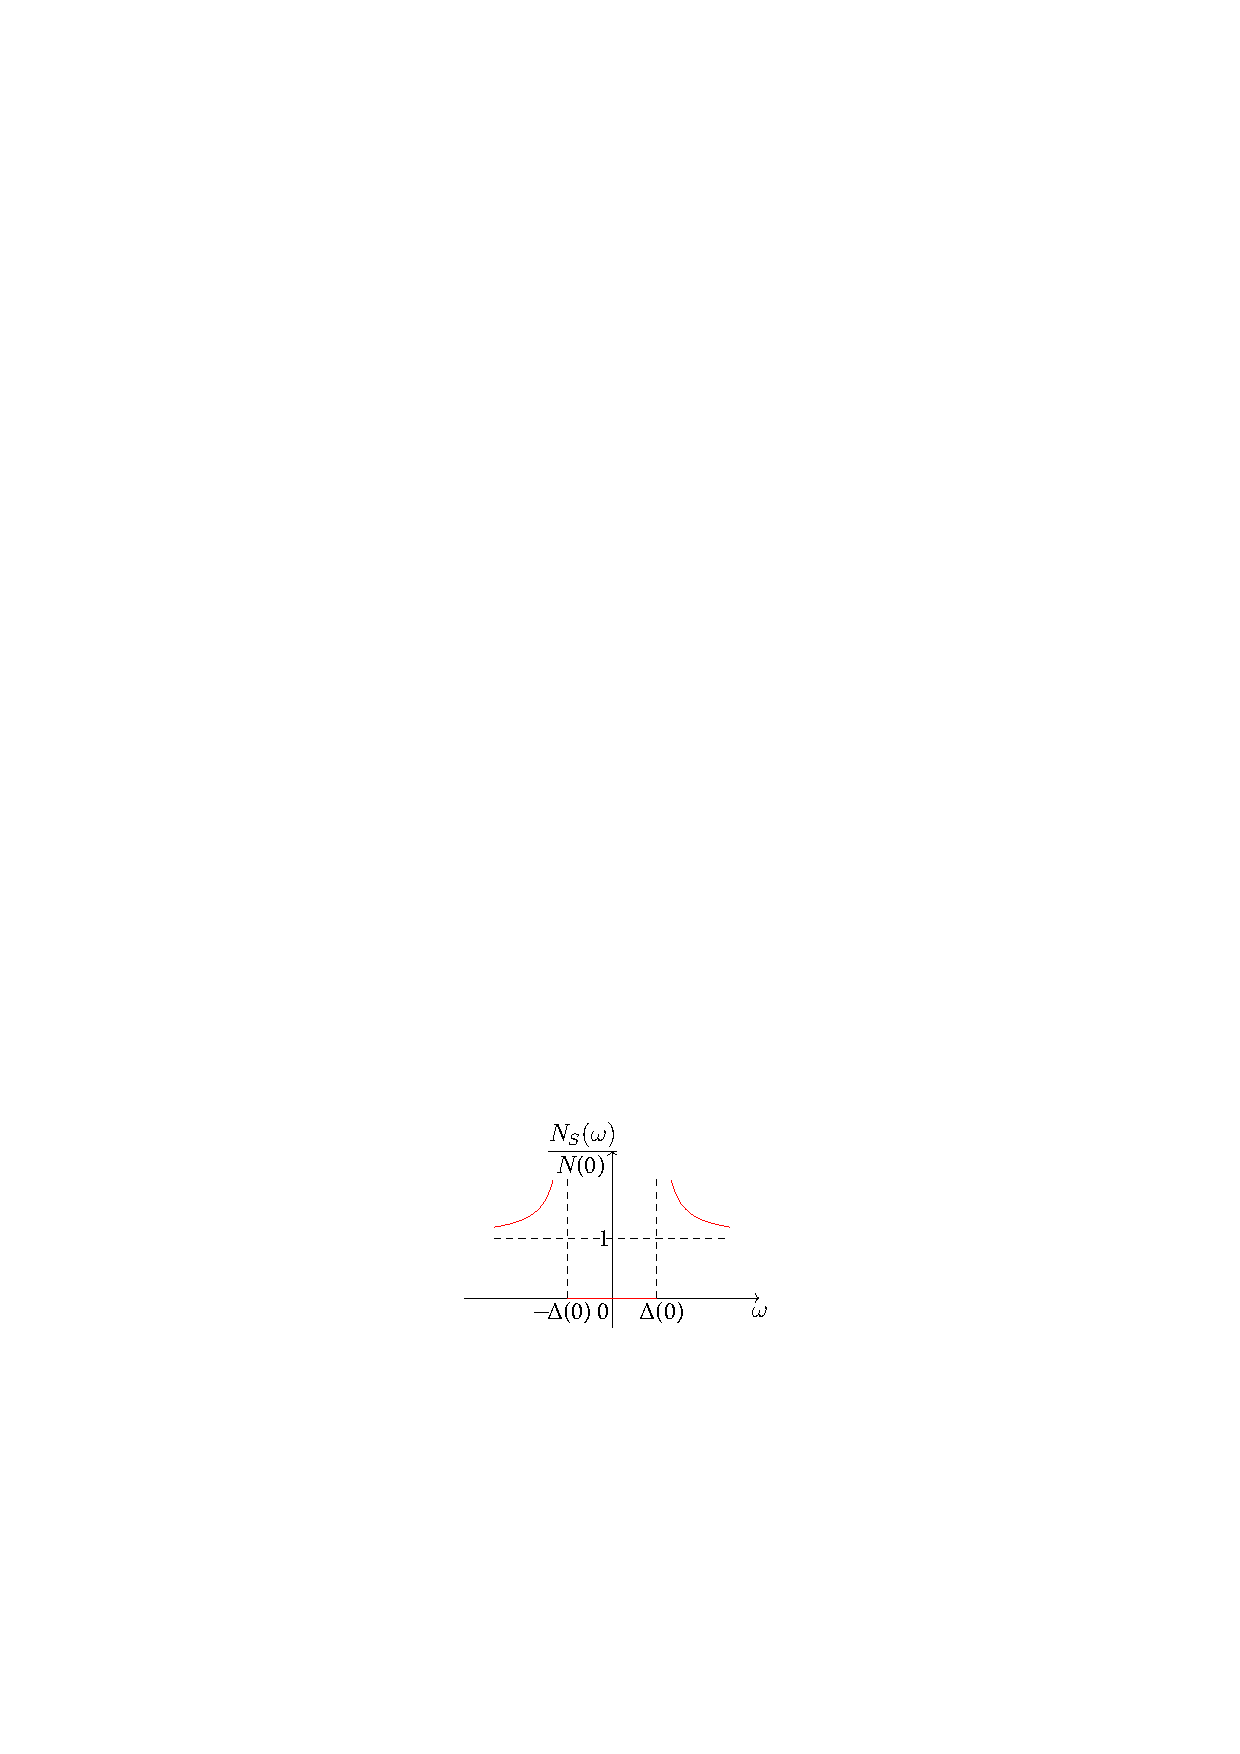
\includegraphics[width=7cm]{figure/sc4.pdf}
    \caption{超导电子态密度分布.}
    \label{sc4}
\end{figure}

另外, 根据谱定理, 有 
   \begin{align}
        \llag \hat{C}_k^\dg \hat{C}_k^{ } \rrag=&2\sum_k\int_{-\infty}^{\infty}\frac{-\frac{1}{\pi}\fun{Im}G^{R}(\vct{k},\omega)}{\e^{\beta\omega}+1}\dd\omega\nonumber\\
        \equiv &2\int\dd\omega n_{\fun{F}}(\omega)N_{\fun{S}}(\omega),
    \end{align}
从而有 
\begin{equation}
    N_{\fun{S}}(\omega)=\sum_k-\frac{1}{\pi}\fun{Im}G^R(\vct{k},\omega),
\end{equation}
这与前面得到的结果一致. 
